%%%%%%%%%%%%%%%%%%%%%%%%%%%%%%%%%%%%%%%%%%%%%%%%%%%%%%%%%%%%%
%% HEADER
%%%%%%%%%%%%%%%%%%%%%%%%%%%%%%%%%%%%%%%%%%%%%%%%%%%%%%%%%%%%%

\documentclass[a4paper,10pt,twoside]{report}
\usepackage{a4}

%% Deutsche Anpassungen

\usepackage[ngerman]{babel}
\usepackage[T1]{fontenc}
\usepackage[utf8]{inputenc}
\usepackage{lmodern}

\usepackage{parskip}
\usepackage{ragged2e}

%% Packages für Grafiken & Abbildungen & Pdf-Dateien & Zitieren


\usepackage{biblatex}
\addbibresource{document.bib}

\usepackage{graphicx} 
\usepackage{wrapfig}
\usepackage{lipsum}
\usepackage{subfig}
\usepackage{tikz}
\usepackage{pdfpages}
\usepackage{floatrow}


%% Packages für Formeln

\usepackage{amsmath}
\usepackage{amssymb,amscd}
\usepackage{amsthm}
\usepackage{amsfonts}
\usepackage{hyperref}
\usepackage[all]{hypcap}
\usepackage{mathrsfs}
\usepackage{tabls}
\usepackage{tabu}
\usepackage{booktabs}
\usepackage{amsthm}

%% Packages für Tabellen

\usepackage{longtable}
\usepackage{tabularx}
\usepackage{array}
\usepackage[a4paper,width=150mm,top=25mm,bottom=25mm]{geometry}
\usepackage{pdfpages}

%% Packages für Listings

\usepackage{listings}
\usepackage{pythonhighlight}
\usepackage{xcolor}
\usepackage{color}
\usepackage{colortbl}

%% Ändern des Heads bei Kapitelseiten

\usepackage{etoolbox}
\patchcmd{\chapter}{\thispagestyle{plain}}{\thispagestyle{fancy}}{}{}

%% Fancy Kopf- und Fußzeilen

\usepackage{fancyhdr}
\pagestyle{fancy}
\fancyhf{}
\setlength{\headheight}{26pt}
\fancyhead[LE, RO]{2020/21}
\fancyhead[CO]{\nouppercase{\rightmark}}
\fancyhead[CE]{\nouppercase{\leftmark}}
\fancyhead[RE, LO]{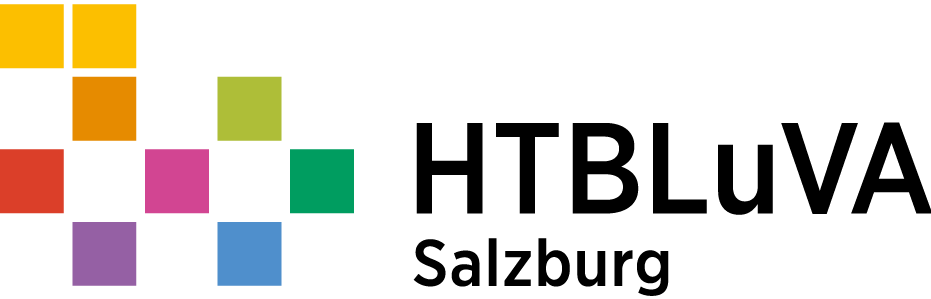
\includegraphics[scale=0.08]{figures/allgemein/HTBLuVA_Salzburg_Logo.png}}
\fancyfoot[LE, RO]{5AHET}
\fancyfoot[C]{Kronberger, Lackner, Kern, Schmeisser}
\fancyfoot[RE, LO]{Seite \thepage}
\renewcommand{\headrulewidth}{0.5pt}
\renewcommand{\footrulewidth}{0.5pt}
\fancypagestyle{plain}{\fancyfoot[C]}

%% Brüche kürzen

\usepackage{cancel}

%% Ändern der Kapitelnummerierung

\renewcommand{\thechapter}{\Roman{chapter}}
	\renewcommand\thesection{\arabic{section}}
		\renewcommand\thesubsection{\thesection.\arabic{subsection}}
			\setcounter{secnumdepth}{3}
			\setcounter{tocdepth}{3}


\definecolor{mygreen}{rgb}{0,0.6,0}
\definecolor{mygray}{rgb}{0.5,0.5,0.5}
\definecolor{mymauve}{rgb}{0.58,0,0.82}

\lstset{ 
	backgroundcolor=\color{white},   % choose the background color
	basicstyle=\footnotesize,        % size of fonts used for the code
	breaklines=true,                 % automatic line breaking only at whitespace
	captionpos=b,                    % sets the caption-position to bottom
	commentstyle=\color{mygreen},    % comment style
	escapeinside={\%*}{*)},          % if you want to add LaTeX within your code
	keywordstyle=\color{blue},       % keyword style
	stringstyle=\color{mymauve},     % string literal style
}

\lstdefinelanguage{JavaScript}{
	keywords={typeof, new, true, false, catch, function, return, null, catch, switch, var, if, in, while, do, else, case, break},
	keywordstyle=\color{blue}\bfseries,
	ndkeywords={class, export, boolean, throw, implements, import, this},
	ndkeywordstyle=\color{darkgray}\bfseries,
	identifierstyle=\color{black},
	sensitive=false,
	comment=[l]{//},
	morecomment=[s]{/*}{*/},
	commentstyle=\color{purple}\ttfamily,
	stringstyle=\color{red}\ttfamily,
	morestring=[b]',
	morestring=[b]"
}



%%%%%%%%%%%%%%%%%%%%%%%%%%%%%%%%%%%%%%%%%%%%%%%%%%%%%%%%%%%%%
%% DOKUMENT
%%%%%%%%%%%%%%%%%%%%%%%%%%%%%%%%%%%%%%%%%%%%%%%%%%%%%%%%%%%%%

\begin{document}
	
\thispagestyle{empty}
\parindent 0pt

%% Deckblatt %%%%%%%%%%%%%%%%%%%%%%%%%%%%%%%%%%%%%%%%%%%%%%%%

% Beginn - Formatierung der Titelseite
\vspace*{20mm}
\begin{center} 
\begin{Huge}\textbf{Diplomarbeit}\end{Huge} \par \bigskip 
\begin{Large}Höhere Technische Bundeslehr- und Versuchsanstalt Salzburg \par \medskip 
Abteilung für Elektrotechnik\end{Large} 
\vspace*{20mm}

\begin{Huge}
\textbf{Entwicklung eines emissionsfreien Sportmotorrades \\[1ex]}
\end{Huge}
\vspace{\fill}

\begin{tabular}{lll}
\multicolumn{3}{l}{\textbf{Entwicklung der Zentralsteuerung / Projektleitung}} \\
 Martin Kronberger & 5AHET & Betreuer: Dipl.-Ing. (FH) Johannes Ferner\\
      &       &      \\
\multicolumn{3}{l}{\textbf{Entwicklung des Antriebssystems}}\\
Jakob Lackner & 5AHET & Betreuer: Prof. Dipl.-Ing. MBA Adolf Reinhart \\
      &       &      \\
\multicolumn{3}{l}{\textbf{Entwicklung des Akkusystems}} \\
Simon Kern & 5AHET & Betreuer: Prof. Dipl.-Ing. Reinhold Benedikter\\
      &       &      \\
\multicolumn{3}{l}{\textbf{Entwicklung der mechanischen Komponenten}} \\
Tobias Schmeisser & 5AHET & Betreuer: Prof. Dipl.-Ing. Peter Lindmoser\\
\end{tabular}
\end{center}
\vspace{\fill}

\begin{minipage}{0.49\textwidth}
Höhere Technische Bundeslehr-\\
und Versuchsanstalt Salzburg \par \medskip 
Itzlinger Hauptstraße 30 \par \medskip 
A-5022 Salzburg \par \medskip 
www.htl-salzburg.ac.at
\end{minipage}
\begin{minipage}{0.49\textwidth} \hspace*{\fill}
{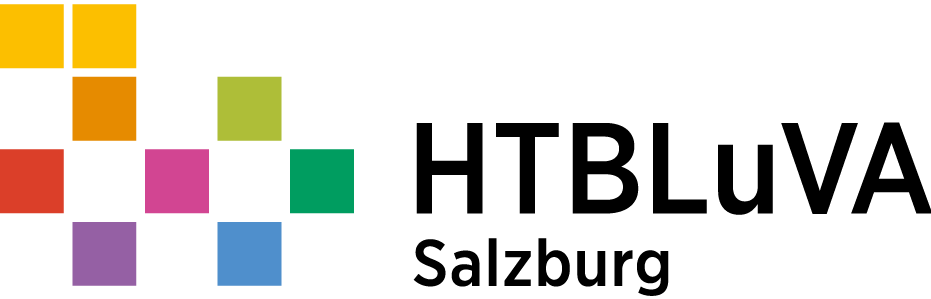
\includegraphics[scale=0.25]{figures/allgemein/HTBLuVA_Salzburg_Logo.png}} \hspace{\fill}
\end{minipage}
\newpage
\clearpage
\thispagestyle{empty}
\mbox{}
\newpage

%% Prolog %%%%%%%%%%%%%%%%%%%%%%%%%%%%%%%%%%%%%%%%%%%%%%%%%%%

\pagenumbering{Roman}
%% Eidestattliche Erklärung
\begin{center}
\begin{huge}
\textbf{Eidesstaatliche Erklärung}
\end{huge}
\end{center}

\bigskip
\justifying{
Wir erklären an Eides statt, dass wir die vorliegende Arbeit selbstständig und ohne fremde
Hilfe verfasst, andere als die angegebenen Quellen nicht benutzt und die den benutzten Quellen
wörtlich und inhaltlich entnommenen Stellen als solche kenntlich gemacht haben. Wir versichern,
dass wir dieses Diplomarbeitsthema bisher weder im In- noch im Ausland (einer Beurteilerin
oder einem Beurteiler) in irgendeiner Form als Prüfungsarbeit vorgelegt haben.}
\vspace{2cm}

%% Gender Erklärung
\begin{center}
\begin{huge}
\textbf{Gendererklärung}
\end{huge}
\end{center}

\bigskip
\justifying{
Aus Gründen der besseren Lesbarkeit wird in dieser Diplomarbeit die Sprachform
des generischen Maskulinums angewendet. Es wird an dieser Stelle darauf hingewiesen,
dass die ausschließliche Verwendung der männlichen Form geschlechtsunabhängig
verstanden werden soll.}
\vspace{2cm}

%% Unterschriften
\begin{center}
\noindent
\begin{tabular}{ll}
\makebox[2.5in]{\hrulefill} & \makebox[2.5in]{\hrulefill}\\
Martin Kronberger & Ort, Datum\\[8ex]
\makebox[2.5in]{\hrulefill} & \makebox[2.5in]{\hrulefill}\\
Jakob Lackner & Ort, Datum\\[8ex]
\makebox[2.5in]{\hrulefill} & \makebox[2.5in]{\hrulefill}\\
Simon Kern & Ort, Datum\\[8ex]
\makebox[2.5in]{\hrulefill} & \makebox[2.5in]{\hrulefill}\\
Tobias Schmeisser & Ort, Datum\\[8ex]
\end{tabular}
\end{center}

%% Leere Seite
\newpage
\thispagestyle{empty}
\mbox{}
\newpage

%% Vorwort
\begin{center}
\begin{huge}
\textbf{Vorwort}
\end{huge}
\end{center}

\bigskip
\justifying{In immer mehr Großstädten werden Fahrzeuge mit Verbrennungsmotoren verboten. Viele Motorräder und Autos können nicht mehr produziert werden, da sie die immer strenger werdenden Abgasnormen nicht mehr einhalten können und das Thema der Klimaerwärmung wird immer präsenter und immer mehr Menschen versuchen ihren „carbon footprint“ zu verkleinern.
\medskip \\ 
Doch leider gibt es für Motorradfahrer zumeist keine wirklichen Möglichkeiten, um für ihr Hobby auf eine emissionsfreie Alternativen umzusteigen. Denn zumeist ist das Preis-Leistungsverhältnis, oder auch das Produkt selbst, nicht sehr einladend. Daher ist unser Ziel die Entwicklung in diesem Bereich voranzutreiben und dadurch den Markt zu vergrößern, wodurch immer mehr und bessere Produkte angeboten werden können.}

%% Leere Seite

\newpage
\thispagestyle{empty}
\mbox{}
\newpage

\begin{center}
\begin{huge}
\textbf{Danksagung}
\end{huge}
\end{center}
\vspace{1cm}

Zu Beginn möchten wir uns bei unseren Betreuern besonders bedanken. Prof. Dipl.-Ing. MBA Adolf Reinhart unterstütze Jakob Lackner in vielen Bereichen, unter anderem konnte er ihm in Bezug auf den Elektromotor fachlich immer weiterhelfen. Prof. Dipl.-Ing. Reinhold Benedikter könnte Simon Kern bei der Dimensionierung und Recherche, im Bereich des Akkusystems, besonders weiterhelfen. Außerdem war Herr Benedikter bereit allerlei Fragen, so fern es möglich war, zu beantworten und bereit uns weiterzuhelfen. Prof. Dipl.-Ing. Peter Lindmoser unterstützte Tobias Schmeisser bei der mechanischen Umsetzung des Konzepts und war für jegliche Fragen immer offen. Dipl.-Ing. (FH) Johannes Ferner unterstützte Martin Kronberger bei den softwaretechnischen Auslegungen und stand bei diversen Problemen immer zur Verfügung.

Einen großen Anteil der Verwirklichung unseres Projektes ist der Firma Schrack for Students anzurechnen. Neben der Finanziellen Unterstützung durch die Firma Schrack for Students hatten unsere Ansprechpartner auch immer ein offenes Ohr für uns bei etwaigen Problemen.

\begin{figure}[H]
	\begin{center}
		
\includegraphics[scale=0.5]{figures/allgemein/Schrack_Logo.jpg}
		\caption{Sigmatek Logo}
	\end{center}
\end{figure}

Für mechanische Komponenten, möchten wir uns bei den Firmen Theodor Wimmer GmbH aus Hof bei Salzburg und G.O. Nilsson Ges.m.b.H. SKF - Vertragshändler aus Wals bedanken. Bei der Firma Theodor Wimmer GmbH möchten wir uns ganz besonders bei Gerlinde und Theodor Wimmer bedanken, welche uns nicht nur mit Bauteilen unterstützen, sondern uns auch bei der Suche nach weiteren Firmen für dieses kostspielige Unternehmen, tatkräftig unterstützten und für Fragen jederzeit erreichbar waren. Bei der Firma G.O. Nilsson Ges.m.b.H. möchten wir Herrn Michael Kudrna nicht unerwähnt lassen, welcher die Ansprechperson für Tobias Schmeisser bei diversen Bauteilen für das Getriebe war.

\begin{figure} [H]
	\begin{center}
		
\includegraphics[scale=0.5]{figures/mechanik/Sponsoren.jpg}		
	\end{center}
\end{figure}
\vspace{0,5cm}
	
Besonders für die informelle Unterstützung im Bezug auf die technische Auslegung, Konfiguration und Programmierung des Curtis Controllers möchten wir uns auch bei den Technikern (Bereich E-Mobilität) Daniel Kramser, Sebastian Bayer und Wolfgang Strasser bedanken.

\newpage
Zusätzlich bedanken wir uns für die finanzielle Unterstützung bei unserem Projekt bei folgenden Firmen:

\begin{figure}[H]
	\begin{center}
		
\includegraphics[scale=0.5]{figures/allgemein/Elin Logo.png}
	\end{center}
\end{figure}
Speziell möchten wir uns bei Ing. Thomas Meister, für die informelle Unterstützung in Bezug auf das gesamte Akkusystem, bedanken.
\vspace{1cm}

\begin{figure}[H]
	\begin{center}
		
\includegraphics[scale=0.7]{figures/allgemein/Sigmatek_LOGO.jpg}
		\caption{Sigmatek Logo}
	\end{center}
\end{figure}

%% Leere Seite

\newpage
\thispagestyle{empty}
\mbox{}
\newpage

%% Abstract Deutsch

\centering
\begin{huge}
\textbf{DIPLOMARBEIT}
\end{huge}

\begin{large}
DOKUMENTATION
\end{large}

\begin{center}
\begin{table}[H]
	\begin{tabular}{|l|l|l|}
		\hline
		Namen der Verfasser &
		\multicolumn{2}{l|}{\begin{tabular}[c]{@{}l@{}}Martin Kronberger, Jakob Lackner,\\ Simon Kern, Tobias Schmeisser\end{tabular}} \\ \hline
		\begin{tabular}[c]{@{}l@{}}Jahrgang\\ Schuljahr\end{tabular} &
		\multicolumn{2}{l|}{\begin{tabular}[c]{@{}l@{}}5AHET\\ 2020/21\end{tabular}} \\ \hline
		Thema der Diplomarbeit &
		\multicolumn{2}{l|}{Entwicklung eines emissionsfreien Sportmotorrades} \\ \hline
		Kooperationspartner &
		\multicolumn{2}{l|}{Schrack for Students, Sigmatek EBG GmbH,} \\ \hline
		Aufgabenstellung &
		\multicolumn{2}{l|}{\begin{tabular}[c]{@{}l@{}}Es soll ein vollständig elektrifiziertes E–Motorrad aus einen\\ alten Model mit Verbrennungsmotor entwickelt werden.\\ Der vorherige Verbrennungsmotor wird durch eine\\ elektrische Steuer und Motoreinheit ersetzt. Ebenfalls soll\\ das Zweirad über ein eigenständiges Akkusystem, mit einem\\ für das Motorrad individuellem Ladesystem verfügen. Über\\ eine zentrale Steuereinheit wird die Kommunikation\\ zwischen den Systemen und dem Menschen gewährleistet.\end{tabular}} \\ \hline
		Realisierung &
		\multicolumn{2}{l|}{\begin{tabular}[c]{@{}l@{}}Als Chassie wird eine ausgeschlachtete Duacati Monster S4 2001\\ verwendet und mit einem eigensentwickelten Rahmen versehen.\\ Angetrieben wird das Motorrad  über eine bürstenlose\\ Synchronmaschine, welche über ein BMS gesteuertes 50,4 Volt\\ Lithiumionen Akkupack versorgt wird. Das Moment wird vom\\ Motor über ein Kettengetriebe mit eine Übersetzung von\\ ungefähr 1/9 auf die Straße übertragen. Die Peripherie wird über\\ einen Raspberry Pi Minicomputer und Taster am Lenker gesteuert.\\ Ebenso wird über ihn die Benutzeroberfläche gesteuert, welche\\ über ein 11,6 Zoll Touch Panel angezeigt und gesteuert werden kann.\end{tabular}} \\ \hline
		Ergebnisse &
		\multicolumn{2}{l|}{\begin{tabular}[c]{@{}l@{}}Zum Abgabezeitpunkt befindet sich die Komponenten des Motorrads\\ im Entwicklungszustand. Der Rahmen ist noch in der Endphase der\\ Fertigung. Der Motor und dessen Software ist Einsatzbereit und\\ müsste nur mehr eingebaut werden. Die Versorgung ist zu ende\\ entwickelt und muss ebenso nur mehr gefertigt werden. Die\\ Steuerung der Benutzeroberfläche befindet sich im Prototypen-Status,\\ beinhaltet jedoch noch einige experimentelle Funktionen, welche noch\\ etwas Programmier und Testzeit benötigen. Gesamt ist das gesamte\\ Konzept vollständig und kann mit etwas mehr Zeit und Sponsorengelder\\ fertiggestellt werden.\end{tabular}} \\ \hline
		\begin{tabular}[c]{@{}l@{}}Möglichkeit der Einsicht-\\ nahme in die Arbeit\end{tabular} &
		\multicolumn{2}{l|}{\begin{tabular}[c]{@{}l@{}}Die Diplomarbeit ist in gebundener Form sowohl in der Schulbibliothek\\ als auch bei AV Prof. Dipl-Ing. (FH) Roland Holzer einzusehen.\\ Darüber hinaus besitzt jedes Mitglied des Projektteams eine vollständige\\ Version in gebundener und digitaler Form.\end{tabular}} \\ \hline
		\begin{tabular}[c]{@{}l@{}}Approbation\\ (Datum/Unterschrift)\end{tabular} &
		Prüfer &
		Abteilungsvorstand \\ \hline
	\end{tabular}
\end{table}
\end{center}
%% Abstract Englisch

\newpage
\centering
\begin{huge}
\textbf{DIPLOMA THESIS}
\end{huge}

\begin{large}
DOCUMENTATION
\end{large}

\begin{center}
\begin{table}[H]
	\begin{tabular}{|l|l|l|}
		\hline
		Author(s) &
		\multicolumn{2}{l|}{\begin{tabular}[c]{@{}l@{}}Martin Kronberger, Jakob Lackner,\\ Simon Kern, Tobias Schmeisser\end{tabular}} \\ \hline
		\begin{tabular}[c]{@{}l@{}}Form\\ Academic year\end{tabular} &
		\multicolumn{2}{l|}{\begin{tabular}[c]{@{}l@{}}5AHET\\ 2020/21\end{tabular}} \\ \hline
		Topic &
		\multicolumn{2}{l|}{Development of an emission-free sports motorcycle} \\ \hline
		Co-operation partners &
		\multicolumn{2}{l|}{Schrack for Students, Sigmatek EBG GmbH,} \\ \hline
		Assignment of Tasks &
		\multicolumn{2}{l|}{\begin{tabular}[c]{@{}l@{}}The plan is to develop a fully electrified e-motorcycle.\\ The previous internal combustion engine is replaced by\\ an control unit and electric motor unit. The two-wheeler\\ should also have an independent battery system with a\\ charging system that is individual for the motorcycle.\\ Communication between the systems and humans is\\ ensured via a central control unit.\end{tabular}} \\ \hline
		Realisation &
		\multicolumn{2}{l|}{\begin{tabular}[c]{@{}l@{}}A cannibalized Duacati Monster S4 2001 is used as\\ the chassis and provided with a specially developed\\ frame. The motorcycle is driven by a brushless\\ synchronous machine, which is supplied by a BMS\\ controlled 50.4 volt lithium ion battery pack. The\\ torque is transmitted from the engine to the road\\ via a chain gear with a ratio of  about 1/9. The\\ periphery is controlled via a Raspberry Pi\\ minicomputer and button on the handlebar.\\ It also controls the user interface, which can be\\ displayed and controlled via an 11.6 inch touch panel\end{tabular}} \\ \hline
		Results &
		\multicolumn{2}{l|}{\begin{tabular}[c]{@{}l@{}}The components of the motorcycle are at the time of\\ delivery in the state of development. The framework \\ is still in its final stages Production. The engine and\\ its software are ready for use and would just have to\\ be built in. The supply is over developed and just\\ needs to be manufactured. The Control of the user\\ interface is in the prototype status, however still\\ contains some experimental functions which are\\ still unavailable\end{tabular}} \\ \hline
		\begin{tabular}[c]{@{}l@{}}Accessibility of Diploma\\ Thesis\end{tabular} &
		\multicolumn{2}{l|}{\begin{tabular}[c]{@{}l@{}}The diploma thesis is available in the school library and at\\ Prof. Dipl.-Ing (FH) Roland Holzer's office. Furthermore,\\ each member of the project team has a complete version.\end{tabular}} \\ \hline
		\begin{tabular}[c]{@{}l@{}}Approval\\ (Date/Sign)\end{tabular} &
		Examiner &
		Department Manager \\ \hline
	\end{tabular}
\end{table}
\end{center}

%% Leere Seite

\newpage
\thispagestyle{empty}
\mbox{}
\newpage

%% Erklärung

\newpage
\begin{huge}
\textbf{Erklärung}
\end{huge}
\bigskip

\justifying{Die unterfertigten Kandidaten haben gemäß \S 34 (3) SchUG in Verbindung mit \S 22 (1) Zi. 3 lit. b der Verordnung über die abschließenden Prüfungen in den berufsbildenden mittleren und höheren Schulen, BGBl. II Nr. 70 vom 24.02.2000 (Prüfungsordnung BMHS), die Ausarbeitung einer Diplomarbeit mit der umseitig angeführten Aufgabenstellung gewählt. Die Kandidaten nehmen zur Kenntnis, dass die Diplomarbeit in eigenständiger Weise und außerhalb des Unterrichtes zu bearbeiten und anzufertigen ist, wobei Ergebnisse des Unterrichtes mit einbezogen werden können. Die Abgabe der vollständigen Diplomarbeit hat bis spätestens}

\bigskip
\begin{center}
\begin{large}
03.04.2020
\end{large}
\end{center}
\bigskip

\justifying{beim zuständigen Betreuer zu erfolgen. Die Kandidaten nehmen weiters zur Kenntnis, dass gemäß \S 9 (6) der Prüfungsordnung BMHS nur der Schulleiter bis spätestens Ende des vorletzten Semesters den Abbruch einer Diplomarbeit anordnen kann, wenn diese aus nicht beim Prüfungskandidaten / bei den Prüfungskandidaten gelegenen Gründen nicht fertiggestellt werden kann.}

%% Unterschriften Schüler
\newpage
\begin{small}
\begin{center}
\begin{tabular}{|p{6cm}|p{8cm}|}
\hline
\renewcommand{\arraystretch}{2}
& \\
\textbf{Kandidaten / Kandidatinnen} & \textbf{Unterschrift} \\ 
& \\ \hline
& \\
Martin Kronberger &  \\ 
& \\ \hline
& \\
Jakob Lackner &  \\ 
& \\ \hline
& \\
Simon Kern &  \\ 
& \\ \hline
& \\
Tobias Schmeisser &  \\ 
& \\ \hline
\end{tabular}
\end{center}
\end{small}
\vspace{3cm}

%% Unterschriften Lehrer
\begin{small}
\begin{center}
\noindent
\begin{tabular}{cc}
\makebox[6.35cm]{\hrulefill} & \makebox[6.35cm]{\hrulefill}\\
Prof. Dipl.-Ing. Reinhold Benedikter & Prof. Dipl.-Ing. (FH) Johannes Ferner\\
Prüfer & Prüfer\\[18ex]
\makebox[6.35cm]{\hrulefill} & \makebox[6.35cm]{\hrulefill}\\
Prof. Dipl.-Ing. Adolf Reinhart, MBA  & Prof. Dipl.-Ing. Peter Lindmoser\\
Prüfer & Prüfer\\[18ex]
\makebox[6.35cm]{\hrulefill} & \makebox[6.35cm]{\hrulefill}\\
Prof. Dipl.-Ing. (FH) Roland Holzer & Dipl.-Ing. Dr.tech. Franz Landertshamer\\
Abteilungsvorstand & Direktor\\[18ex]
\end{tabular}
\end{center}
\end{small}
\raggedright
\pagestyle{fancy}

%% Inhaltsverzeichnis %%%%%%%%%%%%%%%%%%%%%%%%%%%%%%%%%%%%%%%

\tableofcontents

%% INPUT FILE %%%%%%%%%%%%%%%%%%%%%%%%%%%%%%%%%%%%%%%%%%%%%%%


\pagenumbering{arabic}

\input{content/ch_einführung}

\chapter{Einleitung}

\section{Motivation}
Seit kurzem ist die E-Mobilität unter anderem ein neuer schulautonomer Schwerpunkt in der Abteilung Elektrotechnik, an der HTBLuVA-Salzburg. Passend zu diesem Schwerpunkt ergab sich die Idee ein Projekt zum Bereich E-Mobilität zu realisieren, um zukünftige Schüler daran zu interessieren.
Die E-Mobilität umfasst Elemente aus der Mechanik, Elektrotechnik, Kunststofftechnik und Informatik, das Projekt sollte so viele wie möglich  davon abdecken und darstellen können. Gleichzeitig soll das Projekt, eine Art von Prototyp für neu entwickelte Elektromotorräder sein und nicht nur als Abschlussprojekt dienen.

Das Umdenken der Gesellschaft von Verbrennungsmotoren auf Elektromotoren hat zur Folge, dass alltägliche Maschinen immer öfter mit Elektromotoren ausgestattet werden. Motorräder in dieser Größenordnung sind bis dato nicht vorhanden oder erhältlich. Es sind einige Firmen mit der Entwicklung dieser beschäftigt und es werden immer öfter neue Produkte präsentiert, doch diese Zeitalter ist erst am Anfang und benötigt noch Zeit.

Für die Herstellung eines zugelassenen Motorrades ist der Umfang einer Diplomarbeit, aus zeitlichen, sowie budgetären Gründen nicht realisierbar und aus diesem Grund Ist diese Projekt ein Prototyp eines vielleicht zukünftigen Elektro-Sport-Motorades, welches die Verwirklichung des Systems wiedergeben soll.

\section{Zielsetzung}
Ziel dieses Projektes war ein funktionierendes Motorrad, ohne Licht, Hupe oder sonstigen Zusatzfunktionen. Es sollte einfach das System funktionieren, welches die Fortbewegung ermöglichen soll. Das Betriebssystem soll Funktionsfähig und die Versorgung über die Akkus sichergestellt sein. 

Am Ende soll ein fahrtüchtiges Elektromotorrad mit den selben Fähigkeit, wie das Original das Ergebnis sein. Das Gewicht sollte wenn möglich reduziert, aber niemals erhöht werden. Die Zulassung wird in den darauffolgenden Jahren mit der Erweiterung von Licht, Hupe, und so weiter in der Studienzeit erlangt werden. Diese Projekt soll das Interesse des Projektteams an einer Entwicklung eines solchen Produkts bei Firmen zeigen, um aus diesen Prototypen einmal ein Produkt werden lassen zu können.

Die Allgemeinen Funktionen sind die allbekannten. Fahren mit Spitzen bis zu 130 km/h, Bremsen, ABS. Bei elektrischen Antrieben kann die Bremsleistung beim bergabfahren wieder in den Akku eingespeist werden. Diese Funktion nennt sich Rekuperation und wird bei Elektroautos schon verwendet und soll natürlich auch bei dem Elektromotorrad vorhanden sein.
\newpage

\section{Topologie des Gesamtsystems}

\subsection{Gesamtansicht}

In den folgenden Abbildungen kann man das zusammengebaute Gesamtsystem des Emissionsfreien-Sportmotorrads begutachten, ebenso kann man die einzelnen Teilbereiche grob erkennen:

\begin{figure} [H]
	\begin{center}
		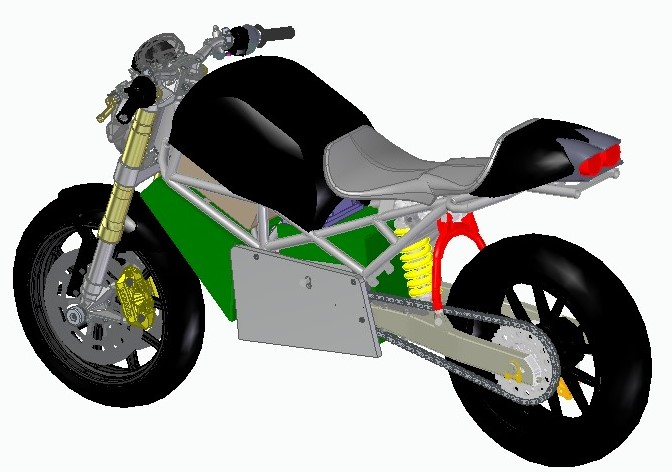
\includegraphics[scale=0.7] {figures/mechanik/Ducati1.jpg}
	\end{center}
\end{figure}

\begin{figure} [H]
	\begin{center}
		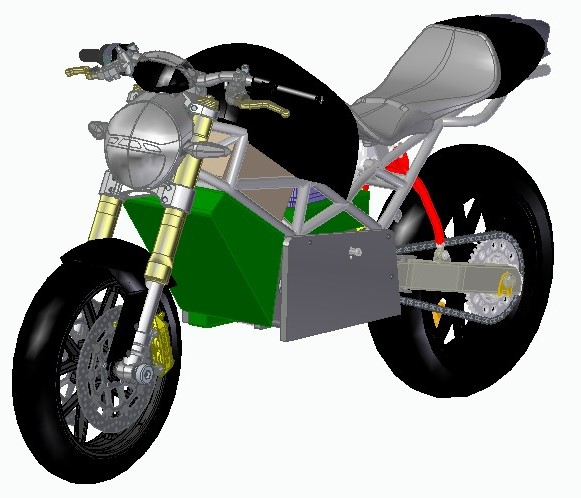
\includegraphics[scale=0.7] {figures/mechanik/Ducati2.jpg}
	\end{center}
\end{figure}

\newpage


\subsection{Projekt-Teilbereiche}
Das gesamte Projekt lässt sich inhaltlich in vier unterschiedliche Teilbereiche gliedern. Der grundsätzliche topologische Zusammenhang der einzelnen Bereiche wird anschließend erläutert:

\begin{figure}[H]
	\begin{center}

		\includegraphics[scale=0.7]{figures/allgemein/GesamtTopologie.png}

	\end{center}
\end{figure}

\begin{figure}[H]
	\begin{center}
		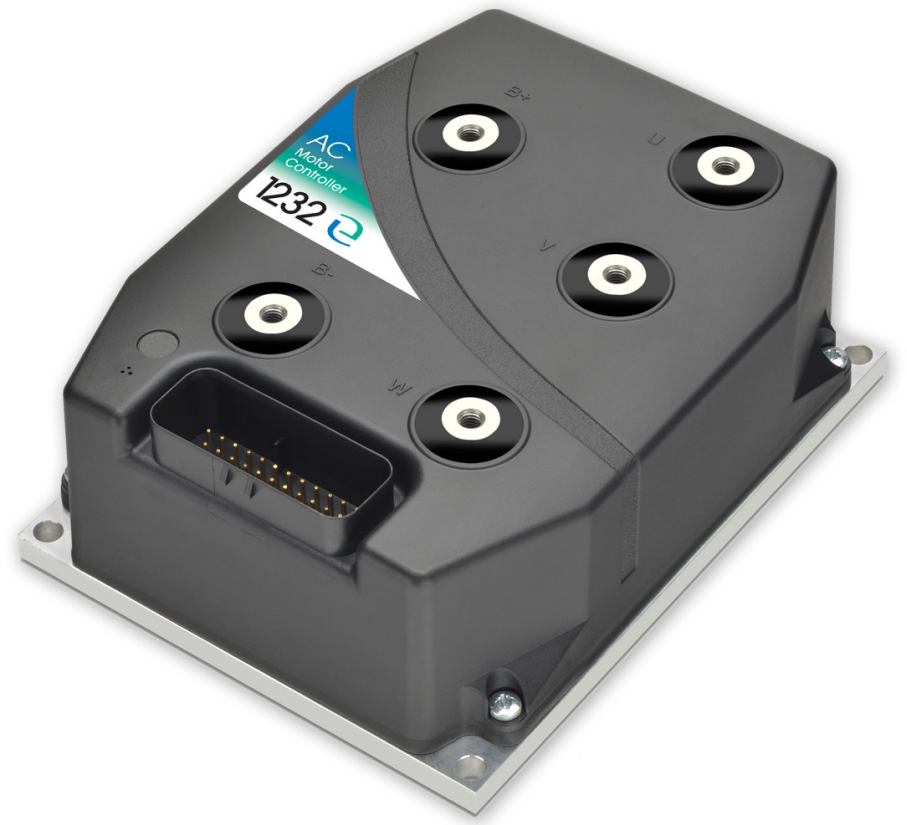
\includegraphics[scale=0.5]{figures/allgemein/Curtis_Controller.png}
		\caption{Curtis Controller}
	\end{center}
\end{figure}


\begin{figure}[H]
	\begin{center}
		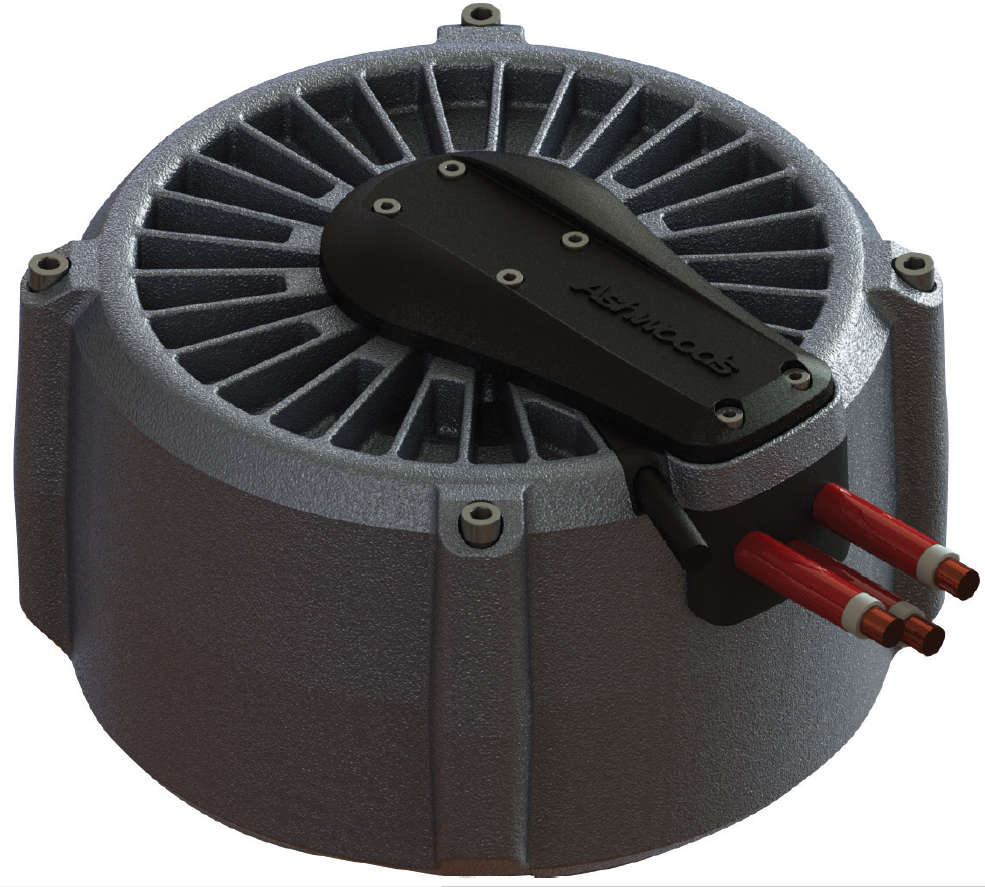
\includegraphics[scale=0.5]{figures/allgemein/Ashwoods_Motor.png}
		\caption{Ashwoods Motor}

	\end{center}
\end{figure}

\begin{figure} [H]
	\begin{center}
		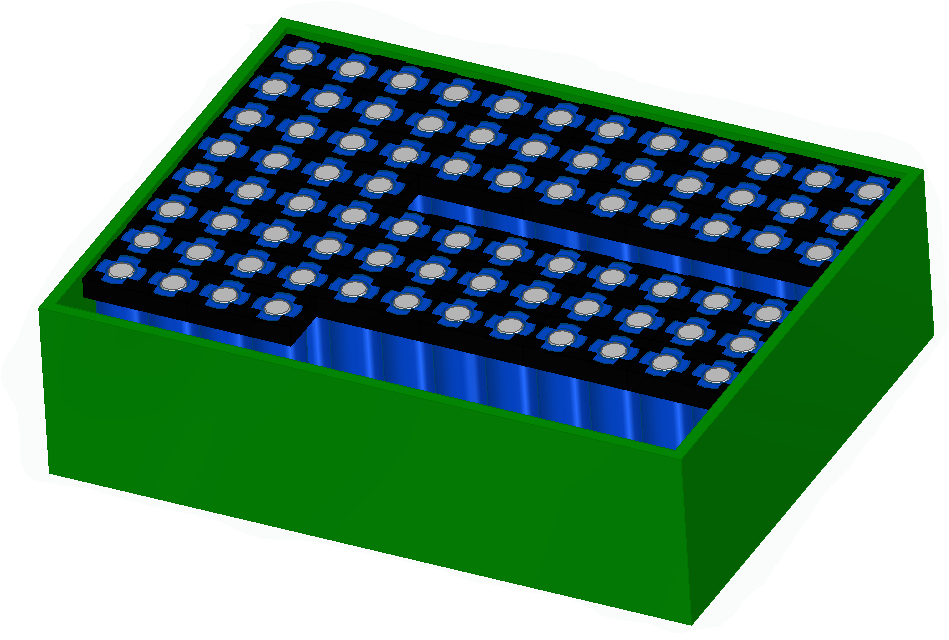
\includegraphics[scale=0.75] {figures/Akku/Akkubox1.PNG}
		\caption{Topologiebild Akkupack}
	\end{center}
\end{figure}

\begin{figure} [H]
	\begin{center}
		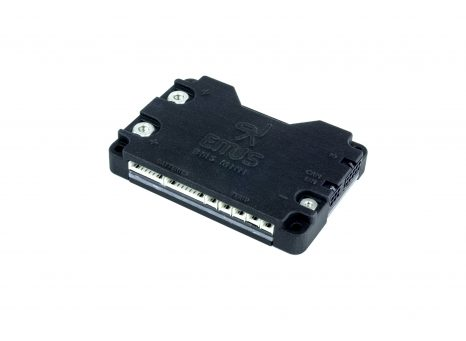
\includegraphics[scale=0.2] {figures/Akku/BMSMINI.jpg}
		\caption{Topologiebild des BMS}
	\end{center}
\end{figure}

Der mechanische Aufbau und die Kraftübertragung stellen die Grundkomponenten eines jeden Motorrads dar, die räumliche Aufteilung der anderen Bauteile wird hier vorgegeben. Die vom Motor umgesetzte Rotationsenergie wird mithilfe des Direkt-Getriebes in kinetische Antriebsenergie (translatorische Beschleunigungsenergie) umgewandelt.

Die Energieversorgung wird mittels eines Akkumulators realisiert, dieser dient als Zwischenspeicher für die durch das Ladegerät hinzugeführten Netzenergie. Das zugehörige Batterie-Management-System ist für die elektrische Kontrolle und notwendige Ladungsausgleiche der einzelnen Li-Ion-Zellen zuständig und steuert die Versorgung der weiteren Betriebsmittel, zusätzlich findet ein Datenaustausch mit den anderen Steuereinheiten über den CAN-Bus statt.

Der Antrieb ist ebenso ein essenzieller Teil des Elektro-Motorrads, da die durch den Akkumulator zur Verfügung gestellte elektrische Energie mithilfe des Motorcontrollers im Motor in mechanisch nutzbare Rotationsenergie umgewandelt wird. Benutzerinteraktionen und Steuermöglichkeiten werden mithilfe der umfassenden Ein- und Ausgänge realisiert.

Die zentrale Steuereinheit sorgt für ein reibungsloses Interagieren der anderen Steuerkomponenten und steuert allgemeine Schaltprozesse. Ein umfangreiches benutzerfreundliches Fahrerlebnis wird durch das Touch-Paneel geboten, weiters wird dadurch eine genaue aber übersichtliche Fahrdatenauswertung während des Betriebs ermöglicht. Der Raspberry PI speichert die gesamte CAN-Bus Kommunikation und sämtliche Benutzerkonfigurationen, um eine vollständige Daten- und Fehlerauswertung im Hinblick auf spätere Wartungen, Optimierungen und Weiterentwicklungen durchführen zu können.

\subsection{Topologischer Überblick}

\newpage

\section{Leitfaden}

Die folgenden Kapitel dieses Dokuments beschreiben die verschiedenen Aspekte des Projekts im Detail. 

In Kapitel \ref{Stand der Technik} ist der Stand der Technik, der verwendeten Technologien, sowie kleinere Auszüge von Normen vorhanden. Dieses Kapitel soll einen Überblick über die Technologien gegeben. Auf dieses Kapitel folgen die Kapitel zur Beschreibung des "Emissionslosen Sportmotorrades". 

In Kapitel \ref{Mechanische Umsetzung} wird als erstes auf die mechanische Umsetzung von Gehäuse, Getriebe, Akkupacks, Akkukühlung und der Zusammenbau dieser Komponenten eingegangen. 

Kapitel \ref{Akku und Ladekonzept} handelt vom Akku- und Ladekozept, in dem eine Übersicht über die Aufgaben der Energieversorgung und des Batteriemanagement gegeben, sowie Die Energieversorgung dokumentiert ist. 

Anschließend beschreibt Kapitel \ref{Antriebsstrang} die Übersicht, den Hardwareaufbau,den Softwareaufbau und die Inbetriebnahme des Antriebsstranges und gibt Einblicke in die Entwicklung der Motorsteuerung. 

Als letztes wird in Kapitel \ref{Zentralsteuerung} Das Human-Computer-Interaction-System Beschrieben. Diese Kapitel beinhaltet die Beschreibung der Zentralsteuerung mit Fahrdatenspeicher, der Benutzeroberfläche am Display und Kommunikation mit der Motorsteuerung, die für den Betrieb entwickelt worden sind.

In nachfolgenden Teilbereichen gilt in den einzelnen Kapiteln eine interne Referenzierung auf einen Unterpunkt in selbigem Kapitel – heißt: „siehe Abschnitt 2.3“ bedeutet, dass besagter Punkt innerhalb des Kapitels nachzuschlagen ist.Wird allerdings auf Abschnitte oder Abbildungen verwiesen, die sich in einem anderen Kapitel befinden, so wird dies beispielsweise als „siehe Kapitel Stand der Technik Abschnitt 2.1.3“ angegeben. Die Namen der Kapitel sind dabei stets mit kursiver Schrift hervorgehoben, um eine bessere Lesbarkeit zu schaffen.

\chapter{Stand der Technik}

%%%%%%%%%%%%%%%%%%% Mechanik

\fancyfoot[C]{Schmeisser}

\section{Kühlung} 

Bei dem Vorgang der Kühlung oder Abkühlung, wird einem System Wärme, oder thermische Energie entzogen. (Deshalb auch Entwärmung genannt)
Unter Kühlung versteht man die Übertragung von Wärme einer technischen Komponente, an die Umwelt. Das Phänomen der Kühlung wird und kann auch beabsichtigt hervorgerufen werden, um bestimmte temperaturabhängige Eigenschaften erreichen und erhalten, aber auch Systeme vor Überhitzung schützen zu können. \footnote{vgl. \cite{Kuehlung1} S.8-28} \footnote{vgl. \cite{Kuehlung2}}

\subsection{Thermodynamische Grundlagen}

Bei Feststoffen und Flüssigkeiten geht der Entzug von Wärme durch Wärmeübertragung entsprechend einem Temperaturgradienten vonstatten. Die wesentlichen Prozesse sind dabei Wärmeleitung und Wärmestrahlung, eingeschränkt auch die Konvektion. Diese Prozesse laufen spontan ab und deshalb, entsprechend der Gesetzen der Thermodynamik, einen Temperaturausgleich zur Folge haben. Diese Phänomen, kann für eine erwünschte Kühlung ausgenützt werden, jedoch ist hierfür viel Energie notwendig.  

Weil durch den Wärmeaustausch die Wärme nach Außen gelangt, hat dies eine Erhöhung der Temperatur, der Umgebung zur Folge. Dies bedeutet eine Umwandlung von Energieformen höherer Ordnung, in thermische Energie. Eine Kühlung im Sinne einer Reduzierung der thermischen Energie eines abgeschlossenen Systems ist daher nicht möglich, was sich in der Praxis zum Beispiel darin äußert, dass auch Kühlschränke letztlich die Temperatur (der Umgebung) erhöhen und nicht senken, wenn dies auch lokal der Fall sein mag.

Bei Festkörpern, ähnlich wie die elektrische Leitfähigkeit, gibt es auch bei der Wärmeleitung Einflussfaktoren. Diese sind hier Wärmeleitkoeffizient, Wärmeübergangskoeffizient und Wärmekapazität. Bei Flüssigkeiten spielt die Wärmeleitung und Wärmestrahlung ebenfalls eine Rolle, hinzu kommt jedoch die Konvektion als wesentlicher Prozess des Temperaturausgleichs. Bei Gasen dominiert die Konvektion. \footnote{vgl. \cite{Kuehlung1} S.8-28} \footnote{vgl. \cite{Kuehlung2}}

\newpage

\subsection{Technische Anwendung}

Kühlsysteme können nach dem verwendeten Wärmeträgermedium unterteilt werden. Die geläufigsten Arten der Kühlung sind:

\begin{itemize}
	\item Wasserkühlung und
	\item Luftkühlung.
	\item Ölkühlung z.  B. im Automotor und in Hydrauliksystemen (hydraulischen Antrieben) 
	\item Natriumkühlung in Kernkraftwerken
	\item Kühlung durch Peltier-Elemente Kühlung von Prozessoren
\end{itemize}

\subsection{Funktionsweise}

Die Kühlung verwendet diese in den Thermodynamischen Grundlagen genannten Phänomene und führt diese künstlich herbei. Diese basiert auf der Wärmeleitung, vom zu kühlenden Körper mit einem Kühlstoff, durch Gas oder Flüssigkeit und des Abtransports, also der Wärmeströmung. Um Platz zu sparen, werden in manchen Anwendungen, als Abtransport, Heatpipes verwendet. Bei Verbrennungs- und Elektromotoren werden oft6 Flüssigkeitskühlungen verwendet.\footnote{vgl. \cite{Kuehlung1} S.8-28} \footnote{vgl. \cite{Kuehlung2}}

\subsection{Technische Kühlungsbeispiele}

\begin{itemize}
	\item Kühlsysteme von Kraftwerken und chemischen Prozessen
	\item Kühlung in der Klimatechnik
	\item Öl- und Ladeluftkühler im Turbodiesel-Motor
	\item Abgaskühlung in AGR-Systemen (zur Emissionsreduzierung (NOx))
	\item Wasserkühlung eines Automotors
	\item Luftkühlung eines Prozessors
	\item Kühlung für Steuerungen
\end{itemize}

\newpage

\subsection{Wasserkühlung}  \label{Stand der Technik}

Bei einer Wasserkühlung (Flüssigkeitskühlung), wird logischerweise Wasser als primäres Kühlmittel verwendet. Für die Wasserkühlung gibt es sehr viele verschiedene Einsatzmöglichkeiten. Diese Art von Kühlung wird in Elektro- wie auch in Verbrennungsmotoren, Hochöfen, Stromrichtern, Kraftwerken, Computern und vielen weiteren Anwendungen verwendet. \footnote{vgl. \cite{Wasserkuehlung}}

\subsubsection{Wasserkühlung bei elektronischen Geräten}

Röhren bestückte Endstufen werden seit fasst 100 Jahren mit einer Wasserkühlung gekühlt. Um Fehler von und deren Folgen, also Zerstörungen, zu vermeiden, wird bei dieser Art von Wasserkühlung kein normales Wasser verwendet, sondern nur destilliertes deionisiertes Wasser. Herkömmliches Wasser wäre bei dioesen großen Spannungen zu gefährlich. Bei einer Kühlung mit destillierten deionisierten Wasser, wird die Wärme durch einen Wärmeübertrager an einen zweiten Kühlkreislauf, welcher keine bestimmte Reinheit des Wassers besitzen muss, ab. Dieser Kreislauf ist von den hohen Spannungen so weit entfernt, dass keine Überschläge oder Kurzschlüsse mit dem Kühlwasser möglich sind. 

Eine weiter Kühlungsmethode verwendet die Siedekondensationskühlung, welche bei Hochleistungsröhren eingesetzt wird. Hier sind Dampferzeugung und Kondensation räumlich nicht voneinander getrennt. Die Kühlflüssigkeit, also das Kühlwasser fließt durch einen Kühlkanal, welcher mit Nuten versehen ist. Die Nuten sind hin zur Anodeninnenseite gerichtet.
In diesen Nuten entsteht durch die Erwärmung oder Erhitzung Wasserdampf. Der Wasserdampf gelangt nun in den Hauptkühlkanal, wo er durch Verwirbelung wieder kondensiert wird.

Dieser Vorgang geschieht bei Temperaturen von über 100°C und nützt zu gleich den Aggregatzustand flüssig zu gasförmig aus. Durch die hier benötigte Hitze für die Verdampfung, kann durch diese Kühlungsmethode auch bei kleinen Röhren große Wärmemengen abgeführt werden.

Neuere Modelle dieser Sender sind nicht mehr mit einer Wasserkühlung ausgestattet.

Auch in der Leistungselektronik wird eine Flüssigkeitskühlung mit Wasser verwendet. Beispiele für die Leistungselektronik sind Stromrichter für Hochspannungs-Gleichstrom-Übertragung oder auch 
Traktionsstromrichter in Schienenfahrzeugen. \footnote{vgl. \cite{Wasserkuehlung}}

\newpage

\subsubsection{Wasserkühlung in Personal Computern}

Sehr oft sind mittlerweile auch Wasserkühlungen in PC-Systemen zu finden. Diese Methode ist um einiges leiser und effizienter um einzelne Komponenten zu kühlen, als die herkömmlichen Luftkühlungen mit Ventilatoren. Mit der Wasserkühlung wird meist der Hauptprozessor gekühlt. Neben dem Hauptprozessor, können noch Grafikkarten, Hauptplatinenchipsätze, Festplatten, Netzteile mit dem Transformator, Spannungswandler und RAM-Bausteine in die Wasserkühlung mit einbezogen werden.
Durch die Effizienz der Flüssigkeitskühlung mit Wasser und der immer weiter steigenden Leistungen, auch von Personalcomputern, ist um die Wasserkühlung bei Rechnern ein Markt entstanden.

Vorteile von einer Wasserkühlung sind unter anderem die schon erwähnte Effektivität der Kühlung der Hardware für Übertaktungsspielraum der CPU, durch die verbesserte Kühlung. Wie ebenfalls schon erwähnt funktioniert diese Kühlung sehr leise und beginnt nicht zu laut blasen, wenn eine große Rechenleistung vom PC verlangt wird. Bei der Wasserkühlung wird als Wärmeübertrager, ein Radiator, mit großen, langsam drehenden Lüftern oder ein passiver Radiatoren ohne Lüfter eingesetzt werden.
Noch nicht genannt, erhöht sich mit einer Wasserkühlung die Zuverlässigkeit und Lebensdauer der durch die Kühlung, gekühlten Bausteine. Durch die Verwendung der richtigen Pumpe kann die Methode der Wasserkühlung eine sehr stromsparende sein

Nachteile bringt diese Methode natürlich auch mit sich. Die Wasserkühlung, hat einen erheblich größeren Installationsaufwand und damit auch vergleichsweise hohe Kosten zur Folge. Mit den Genannten Problemen kommt auch noch die Wartung hinzu, weil nicht nur der Ventilator geputzt erden müssen.  Durch den Verzicht der Kühlung von einzelnen Komponenten, kann dies zur Überhitzung der selbigen führen. Mit hinzu kommt auch noch der erheblich größere Platzbedarf im Gehäuse. 

Weil destilliertes Wasser, verglichen mit anderen Kühlungsflüssigkeiten bei Zimmertemperatur, den größten Wärmeleitkoeffizienten besitzt, ist diese Flüssigkeit die erste Wahl bei einer Flüssigkeitskühlung. \footnote{vgl. \cite{Wasserkuehlung}}

\newpage

\subsection{Luftkühlung} 

Elektronische Bauelemente der Leistungselektronik, Verbrennungsmotoren und Klimaanlagen werden bei der Luftkühlung, durch die an den Oberflächen vorbei strömende Luft gekühlt.
Die bei einer Luftkühlung benötigte Luftströmung kann durch verschiedene Arten erreicht werden. Unter andern durch Konvektion, Gebläse, also Ventilatoren, oder bei Fahrzeugen durch den Fahrtwind. 
Das Luftgekühlte Bauteil steht entweder so frei, dass es von Luft umströmt wird oder der Luftstrom wird mittels Kanäle um die Komponente geleitet. Oft sind freistehende Komponenten mit Kühlkörper aus einem Metall oder Kühlrippen als Wärmeübertrager versehen. Durch Rippen wird die Oberfläche vergrößert und dies hat einen größeren Wärmeabtransport zur Folge. \footnote{vgl. \cite{Luftkuehlung1}} \footnote{vgl. \cite{Luftkuehlung2}}

\subsubsection{Luftkühlung bei Personalcomputern}

Mit der Größe eines Prozessors, steigt auch die Wärmeentwicklung. In aktuellen PCs eingebaute leistungsstarke Mikrochips, erzeugen erhebliche Verlustwärme. Diese Wärme wird meist durch eine Luftkühlung abgeführt, um eine thermische Überlastung der Chips zu verhindern.

Um die Wärmeentwicklung zu verringern, wurde die Betriebsspannung der Bauteile reduziert, weil die gesamte Aufnahmeleistung in Wärme umgesetzt wird. Ebenfalls werden bei normalen Betrieb nicht benötigten Bauteilen, die Taktfrequenz verringert oder die Bauteile auch ganz abgeschaltet um weniger oder keine unnötige Energie zu verbrauchen oder unnötige Wärme zu erzeugen. Trotz dieser Methoden, reicht die Abfuhr der Wärme durch Strahlung und Konvektion nicht mehr aus.
Aus diesem Grund müssen Kühlkörper und Ventilatoren benutzt werden. Die Ventilatoren, sind am Rand des Gehäuses mit Luftkontakt nach Außen angebracht. Diese bewirken einen Luftstrom bei den zu kühlenden Komponenten und bläst die Warme Luft nach außen. Gleichzeitig wird kalte Luft von der anderen Seite angesaugt. Dies kann durch Luftlöcher erzwungen werden, die an einem kühltechnisch sinnvollen Platz gewählt worden sin, damit alle Bauteile, die eine Kühlung benötigen, umströmt werden.
Durch die mit gerippten Kühlkörpern vergrößerten Oberfläche der Bauteile ist die Kühlung ausreichend und ein zuverlässiger Betrieb ist möglich. 

In einem Rechner wird die CPU am stärksten gekühlt. Neben der CPU werden auch, wie schon in der Wasserkühlung erwähnt, Prozessoren von Grafikkarten und auch das Netzteil mit Transformator mit gekühlt. Bei einer Luftkühlung natürlich mit der Luft. \footnote{vgl. \cite{Luftkuehlung1}} \footnote{vgl. \cite{Luftkuehlung2}}



Weitere Anwendung:
\begin{itemize}
	\item HiFi-Verstärker 
	 Kunststoff
\end{itemize}

\newpage


\subsection{Aktive Kühlung} 

Bei einer aktiver Kühlung wird eine Kühlung durch eine Pumpe oder einem Lüfter künstlich erzwungen und wird eingesetzt, wenn die Abfuhr der Wärme durch Strahlung und Konvektion nicht mehr ausreicht. \footnote{vgl. \cite{Luftkuehlung1}} \footnote{vgl. \cite{Luftkuehlung2}}

\subsubsection{Aufbau}

Eine aktive Kühlung besteht meist aus den folgenden Komponenten:

\begin{itemize}
	\item Kühlmittel
		\begin{itemize}
        	\item Wasser
         	\item Luft
         	\item Öl
         	\item speziellen Kühlflüssigkeit
     	\end{itemize}
\end{itemize}

Das Kühlmittel sorgt oft auch für die Schmierung der Bauteile. 

\begin{itemize}
     \item Antreibende Komponente
     	\begin{itemize}
        	\item Lüfter
         	\item Pumpe
     	\end{itemize}	
\end{itemize}

Diese Komponenten erzwingen einen Kühlmittelstrom. 
Bei einem Lüfter wird die Luft zu einem Luftstrom gezwungen und umströmt das zu kühlende Bauteil. Bei einer Pumpe fließt das Kühlmittel nicht nur zum zu kühlenden Objekt, sondern ebenfalls durch den Radiator, welcher die Flüssigkeit auf Ausgangstemperatur herunter kühlt. 


Funktionsprinzip einer Aktiven Kühlung entspricht beispielsweise der Wasserkühlung.

Mittels einer Pumpe wird das Kühlmedium (Wasser, Kühlmittel) durch einen Kühlkreislauf, der aus Schläuchen oder Bohrungen (Nuten) besteht durch gepumpt. Am anderen Ende der Zubringleitung befindet sich das Objekt, welches gekühlt werden soll und wird von der Kühlflüssigkeit umflossen. 
Das Kühlmittel nimmt die Wärme auf und transportiert sie ab. Bei der Rückleitung fließt das Wasser durch den Radiator, welcher die Temperatur des Wassers reduziert und eine Erhitzung der Pumpe verhindert. 
Der Radiator gibt die Wärme durch Ventilatoren oder bei einem passiven Radiator durch Strahlung an die Umgebung ab. Dafür ist aber immer ein Temperaturgefälle notwendig, weil sonst eine Abgabe nicht möglich ist. und je größer das Gefälle ist, desto mehr Wärme kann pro Zeit abgegeben werden.\footnote{vgl. \cite{Luftkuehlung1}} \footnote{vgl. \cite{Luftkuehlung2}}

\subsection{Passive Kühlung} 

Die passive Kühlung ist im Grunde jede natürliche Abkühlung von Körpern. Hier wird das Phänomen der Wärmekonvektion verwendet. Diese Kühlung wird verwendet um die Erwärmung eines Motors, oder einer Maschine und elektrischen Geräten an die Umwelt abzugeben. Der Effekt für die Konvektion kann durch Kühlrippen verstärkt werden. Bei jeder aktiven Kühlung, sind also auch passive Kühlungen vorhanden, weil man die Wärme noch nicht "zwingen" kann von einem Köper an die Umgebung abzugeben. 

Eine passive Kühlung benützen zum Beispiel Kühlrippen oder Radiatoren. Diese Elemente bestehen aus Metall und geben die Wärme des wärmeren Mediums an das Kältere weiter. Um eine Beschleunigung zu erlangen, wird eine passive Kühlung mit eingesetzt. \footnote{vgl. \cite{PassiveKuehlung}}

%%%%%%%%%%%%%%%%%%%%%%%%%%%%%%%%%%%%%%%%%%

\newpage

\section{Schutzarten Elektrischer Betriebsmittel} 

Die Schutzart eines Betriebsmittels gibt an, wie gut dieses geschützt ist vor:
\begin{itemize}
	\item Zugang von Personen zu gefährlichen Teilen innerhalb eines Gebäudes
	\item Eindringen von fremden Festkörpern
	\item Eindringen von Wasser
\end{itemize}
 
Die Angabe der Schutzart erfolgt in Form eines Kurzzeichens (IP-Code/ International-Protection-Code)
Dieser Schutz entspricht den Regeln von ÖVE/ÖNORM EN 60529 (und IEC)

Die erste Kennziffer, gibt den Schutz gegen Berührung von gefährlichen Teilen innerhalb des Gehäuses und den Schutz gegen das Eindringen von festen Fremdkörpern an.
Die zweite Kennziffer gibt den Schutz gegen Eindringen von Wasser an. \footnote{vgl. \cite{IPSchutzarten} S.63,64}

\begin{table}[H]
	\begin{tabular}{|c|c|c|c|l}
\cline{1-4}
		\textbf{Schutzart} & \textbf{Betriebsmittelschutz} & \textbf{Personenschutz}    & \textbf{Anwendung}             &  \\ \cline{1-4}
		IP6X               & staubgeschützt                & gegen eindringen von Draht & Deckelverschluss der Akkupacks &  \\ \cline{1-4}
		IPX7               & zeitweilig wasserdicht        & -                          & Gesamtes Akkupack              &  \\ \cline{1-4}
		IPX8               & dauerhaft wasserdicht         & -                          & Akkupack-Korpus                &  \\ \cline{1-4}
	\end{tabular}
	\caption{Auszug IP Schutzarten}
\end{table}


\newpage

\section{Solid Edge}


\begin{figure} [H]
	\begin{center}
		
\includegraphics[scale=0.5]{figures/mechanik/Untitled.jpg}
			\caption{Solid Edge Logo}
			\label{fig:Solid Edge Logo}
	\end{center}
\end{figure}


Dank 1,5 jähriger Ausbildung in den ersten beiden Jahren in der HTBLuVA-Salzburg, konnte als Planungs- und Berechnungsprogramm, Solid Edge verwendet werden. 
Es wurden alle Teile des Motorrades in diesem Programm erstellt und geplant. Bei den Seitenplatten war noch eine Berechnung der Stabilität notwendig; um die Sicherheit prüfen zu können. 

\subsection{Erklärung}

Solid Edge ist ein 3D-Zeichenprogramm aus dem Hause Siemens. Auf einfachsten Wege, können virtuell Teile erstellt, auf Zeichenblättern für die Fertigung gedruckt und mit anderen Teilen zu Geräten miteinander verbunden werden. 

Mit der Funktion "DIN Metrisch Part" können Einzelteile erstellt und dimensioniert werden. In dieser Funktion sind einige Zeichenhilfen vorhanden, die einem das Zeichnen und planen erleichtern. Unter dem Abteilung "Volumenkörper" kann festgelegt werden, wie das Teil später einmal hergestellt werden soll. Beispielsweise wäre ein Rotationsausschnitt eine Fertigungsweise, einer Drehmaschine.


\begin{figure} [H]
	\begin{center}
		\includegraphics[scale=0.4]{figures/mechanik/Solid Edge_Volumenkörper.jpg}
			\caption{Solid Edge Volumenkörper}
			\label{fig:Solid Edge Volumenkörper}
	\end{center}
\end{figure}


Mit "Bemaßen" werden Maße des Formkörpers festgelegt.


\begin{figure} [H]
	\begin{center}
		\includegraphics[scale=0.4]{figures/mechanik/Solid Edge_BemaßenZeichn.jpg}
			\caption{Solid Edge Bemaßen}
			\label{fig:Solid Edge Bemaßen}
	\end{center}
\end{figure}


In der selben Funktion, lassen sich auch Berechnungen durchführen.
Unter der Registerkarte Simulationen, sind alle hierfür notwendigen Werkzeuge zu finden.
Mit "Strukturelle Lasten", können an den gewünschten Punkten, beliebige Arten und Größen von Kräften angelegt werden. 


\begin{figure} [H]
	\begin{center}
		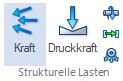
\includegraphics[scale=0.4]{figures/mechanik/Solid Edge_Strukturelle Lasten.jpg}
			\caption{Solid Edge Strukturelle Lasten}
			\label{fig:Solid Edge Strukturelle Lasten}
	\end{center}
\end{figure}


Der nächste Schritt besteht darin eine "Vernetzung" durchzuführen, um die Berechnung zu ermöglichen. Durch die Vernetzung, wird die Kontur des Bauteiles vernetzt, welche bei der Berechnung des Verhalten des Teiles auf die Kräfte, notwendig ist. 


\begin{figure} [H]
	\begin{center}
		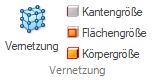
\includegraphics[scale=0.4]{figures/mechanik/Solid Edge_Vernetzung.jpg}
			\caption{Solid Edge Vernetzung}
			\label{fig:Solid Edge Vernetzung}
	\end{center}
\end{figure}


Mit "Berechnen", wird die Berechnung gestartet und das Ergebnis ausgegeben.
Im Ergebnis können die Verschiebung des Teiles, auftretende Spannungen und viele weitere Ergebnisse abgerufen und auch mit "Animation", animiert beobachtet und abgelesen werden. 


\begin{figure} [H]
	\begin{center}
		
\includegraphics[scale=0.4]{figures/mechanik/Solid Edge_Animation.jpg}
			\caption{Solid Edge Animation}
			\label{fig:Solid Edge Animation}
	\end{center}
\end{figure}


Die Funktion "DIN Metrische Zeichnung", kann das Bauteil in 2D Ansichten, für Zeichnungen umgewandelt werden, um das Bauteil fertigen lassen zu können. Die umgewandelten Ansichten können bemaßt und geschnitten werden, um ein bestmögliches Verständnis der Fertigungsabteilung zu versichern. Mit "Ansichtsassistent" kann das gewünschte Teil ausgewält unf umgewandelt werden.


\begin{figure} [H]
	\begin{center}
		
\includegraphics[scale=0.4]{figures/mechanik/Solid Edge_Zeichnungsansichten.jpg}
			\caption{Solid Edge Zeichnungsansichten}
			\label{fig:Solid Edge Zeichnungsansichten}
	\end{center}
\end{figure}


Mit der Funktion "DIM Metrische Baugruppe", können Einzelteile zu einem virtuellem Gerät zusammengebaut werden. Hier wird unter anderem ermöglicht Simulationen von Bewegungs- ,oder Getriebeabläufen zu erstellen. Durch die "Komponentenmontage" werden Beziehungen zwischen Teilen festgelegt und fixiert.

\begin{figure} [H]
	\begin{center}
		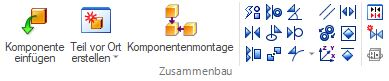
\includegraphics[scale=0.5]{figures/mechanik/Solid Edge_Zusammenbau.jpg}
			\caption{Solid Edge Zusammenbau}
			\label{fig:Solid Edge Zusammenbau}
	\end{center}
\end{figure}
\newpage

\fancyfoot[C]{Kern}

\section{Akkusysteme}
Verschiedene Speicher für elektrische Energie, die auf einer elektrochemischen Basis basieren, nennt man Batterien oder auch Akkumulatoren. Elektrochemische Speicher haben in den vergangenen Jahren immer mehr an Bedeutung gewonnen und werden auch in Zukunft immer öfter Gebrauch finden. Möglich wurde unsere heutige elektronische Mobilität erst mit der Erfindung der galvanischen Zelle. Seit dieser Erfindung, die mit Hilfe eines Stromkreises chemische Energie in elektrische Energie umzuwandeln, hat sich über die jahrzehntelange Weiterentwicklung der Batterie einiges getan. Die Einsatzmöglichkeiten von Akkumulatoren sind extrem vielfältig. Kleine Lithium-Ionen Akkus werden zum Beispiel als Knopfzellen in Smartphones verwendet. Jedoch können sie auch bis hin zu großen stationären Energiespeichern für erneuerbare Energien benutzt werden. Wie bereits vorher erwähnt, sind elektrische Energiespeicher ein wichtiger Bestandteil für den Erfolg der Elektromobilität geworden. Es gibt unzählig viele verschiedene Arten von Batterien, die sich im chemischen Aufbau, ihrer Form und natürlich in ihren Einsatzmöglichkeiten unterscheiden. Durch die äußerst besonderen chemischen Eigenschaften und die vielseitigen Anwendungsbereiche, hat sich der Lithium-Ionen Akku durchgesetzt.
\newpage

\section{Batteriearten}

\subsection{Bleiakkumulator}
Die ersten Versuche, einen auf Blei basierenden Akkumulator zu entwickeln, wurden am Anfang des 19. Jahrhunderts durchgeführt. Industriell wurde der Bleiakku interessant, als Forscher und Chemiker zusammen 1880 ein Verfahren entwickelten, bei dem der Bleiakkumulator bereits nach wenigen Ladezyklen, eine hohe Kapazität erreichte. Der erste technisch einsetzbare Bleiakkumulator wurde 1886 von Henri Tudor entwickelt. Dieser besitzt eine Zellspannung von ungefähr 2V (abhängig vom Ladezustand), was eine durchaus große Spannung für sogenannte wässrige Systeme ist. Der Ausdruck wässrige Systeme leitet sich von dem Elektrolyt ab. Bei Bleiakkumulatoren wird wässrige Schwefelsäure als Elektrolyt verwendet. Im entladenen Zustand bestehen beide Pole aus Blei(II)-sulfat (PbSO4). Weiters besteht die Kathode aus Blei und die Anode aus Bleioxid. Bleiakkumulatoren sollten keinesfalls Tiefenentladen werden, da dies zu Schäden führt und den Akku unbrauchbar macht. Ein extrem großer Nachteil ist das Gewicht, da nur 30 bis 40Wh/kg erreicht werden können.
Diese Art von Akku zeichnet sich durch das kurzzeitige Zulassen hoher Ströme aus die zum Beispiel für Fahrzeug -bzw. Starterbatterien notwendig sind. Unter anderem sind 50 Prozent des Batteriemarktes von Bleiakkumulatoren belegt. Wie vorher bereits erwähnt werden diese oftmals in Autos, LKWs oder auch Motorräder verbaut \footnote{vgl. \cite{Bleiakkumulator}}.

\subsection{Nickel-Metallhybrid Akkumulatoren}
Die technischen Grundlagen des Nickel-Metallhybrid Akkumulator wurden von Stanford R. Ovshinsky und Masahiko Oshitani ab 1962 bis 1982 zur marktreifen Zelle entwickelt. Seit dem Jahr 2006 sind spezielle NiMH-Akkumulatoren auf dem Markt, die sich gegenüber herkömmlichen NiMH-Akkus durch eine deutlich reduzierte Selbstentladung auszeichnen. Die positive Elektrode eines Nickel-Metallhybrid Akkumulators(NiMH) besteht aus Nickel(II)-hydroxid wogegen sich die negative Elektrode aus einem Metallhybrid zusammensetzt. Als Elektrolyt verwendet dieser Akkumulator eine Wasserstoffspeicherlegierung aus Nickel und seltenen Erden. NiMH-Akkus erreichen bis zu 80Wh/kg. Sie sind vielfach in den üblichen Bauformen von Standardbatterien verbreitet und liefern pro Zelle eine Spannung von 1,2V. Oftmals werden sie als wiederaufladbare Alternative der gängigen Alkalibatterien in haushaltsüblichen Geräten eingesetzt. Ein großer Vorteil gegenüber den Nickel-Cadmium Batterien ist es, das der NiMH Akku nicht aus giftigen Cadmium besteht und er außerdem eine höher Energiedichte aufweist.
Der Anwendungsbereich von NiMH Akkumulatoren ist sehr vielfältig. Vorzugsweise kommen sie wie NiCd Akkus überall dort zur Anwendung, wo ein hoher Energiebedarf besteht und hohe Batteriekosten vermeiden werden sollten. Typische Anwendungsbereich sind zum Beispiel Foto- Videogeräte, Elektroautos, Elektrowerkzeuge und noch viele mehr. NiMH Akkus werden außerdem oft als Energiespeicher für Notbeleuchtungsanlagen verwendet \footnote{vgl. \cite{Nickel-Metallhydrid-Akkumulator}}.
\newpage
\subsection{Nickel-Cadmium Akkumulatoren}
1899 wurde der Nickel-Cadmium Akku von dem Schweden W. Jungner entwickelt. NiCd Akkus zeichnen sich dadurch aus, dass sie einen eingebauten Ent- und Überladeschutz integriert haben. Das hat zur Folge, dass man keine aufwendige elektronische Beschaltung durchführen muss. Als Material für die Kathode dieses Akkus verwendet man Nickeloxidhydroxid. Die Anode dagegen besteht aus dem giftigen Material Cadmium, welches jedoch eine äußerst hohe spezifische Ladung (478Ah/kg) besitzt. Bei Nickel-Cadmium Akkumulatoren besteht das Elektrolyt aus Kalilauge. Die typische Nennspannung ist exakt die selbe wie bei NiMH Akkus, 1,2V. Aus dieser Zellenspannung ergibt sich eine spezifische Energie von ungefähr 60Wh/kg. Eine Eigenschaft die man bei anderen Technologien nur selten antrifft ist das hervorragende Tieftemperaturverhalten von NiCd Akkus. Selbst bei einer Temperatur von -40°C ist eine Inbetriebnahme noch möglich. Im Jahr 2004 wurde jedoch die Verwendung von Nickel-Cadmium Akkus wegen dem giftigen Material auf medizinische und sicherheitsrelevante Bereiche begrenzt. Diese Akkumulatoren sind in 2 verschiedenen Bauformen verfügbar, die sich durch die unterschiedlichen Anwendungsbereiche unterscheiden. Die offene Bauweise wird meist für Starterbatterien für Verbrennungsmotoren und Traktionsbatterien für Elektrofahrzeuge verwendet. Bei der anderen Bauweise, werden die Zellen gasdicht verschlossen. Oftmals werden sich für zentrale Stromversorgungssysteme für Notbeleuchtung verwendet \footnote{vgl. \cite{Nickel-Cadmium-Akkumulator}}.
\newpage

\subsection{Lithium-Ionen Batterie}
\subsubsection{Geschichte}
Schon bereits in dem Jahr 1970 wurde von Jürgen Otto Besenhard und anderen das grundlegende Funktionsprinzip der Alkalimetallionen-Interkalation in Kohlenstoff-Elektroden sowie auch in oxidischen Elektroden erforscht und veröffentlicht. Ebenfalls wurde dabei die Anwendung in Lithium Batterien untersucht auch wenn zu der Zeit die praktische Anwendbarkeit als Elektroden für Lithium Batterien noch nicht erkannt wurde. Der erste auf dem Markt erhältliche Lithium-Ionen Akkumulator wurde von Sony im Jahr 1991 angeboten. Dieser Lithium-Cobaltdioxid Akku wurde in einer Videokamera verbaut. Die Batterie, die eine Spannung von 7,2V aufweist, bestand aus zwei seriell verschalteten Zellen und wies etwa eine Kapazität von 1200mAh auf. Sogar bis heute wird diese Bauform von Akkumulatoren mit Kapazitäten
bis zu 6900mAh angeboten und in äußerst vielen Geräten eingesetzt. Drei Physiker bzw. Chemiker (Whittingham, Goodenough und Yoshino) erhielten 2019 sogar den Nobelpreis für Chemie, für die Entwicklung der Lithium-Ionen Batterie.
Forscher einer Universität fanden im Jahr 2020 heraus, dass durch die Zugabe von dem Element Kalium die Lithium Akkumulatoren langlebiger und sicherer werden. Außerdem verhindert das Kalium in dem Akku unerwünschte chemische Nebenreaktionen\footnote{vgl. \cite{Lithium-Ionen-AkkumulatorGeschichte}}.

\subsubsection{Allgemeines}
Es gibt zahlreiche verschiedene Bauformen von Lithium-Ionen Akkumulatoren. Diese Batterien unterscheiden sich nicht nur in ihrer Größe und der Bauform, sondern auch in der chemischen Zusammensetzung ihrer Komponenten und haben unter anderem auch verschiedene Spannungsbereiche. Kenndaten wie Zellenspannung, Lade- und Entladeschlussspannung, Temperaturempfindlichkeit und der maximal zulässige Lade- oder Entladestrom variieren bauartbedingt und sind wesentlich vom eingesetzten Elektrodenmaterial und den Elektrolyten abhängig. Eine Eigenschaft die alle Lithium-Ionen Akkumulatoren gemeinsamen haben ist, dass sie gasdicht versiegelt sein müssen und außerdem lageunabhängig betrieben werden können. Die spezifische Energiedichte liegt ungefähr in der Größenordnung von 150Wh/kg und weist eine Energiedichte von 400Wh/l auf. Durch diese Eigenschaften findet diese Art von Batterie besonderen Einsatz in der mobilen Branche als elektrischer Energiespeicher. Ein weiteres wichtiges Merkmal aller Lithium-Ionen Akkumulatoren ist, dass sie Überladungen nicht verkraften können. Wenn man mehrere Zellen zum Beispiel in Reihe schaltet, um eine höhere elektrische Spannung zu erzielen, müssen zum Ausgleichen der Toleranzen in der Kapazität zwischen den Zellen meistens zusätzlich ein Batteriemanagementsystem (BMS) und ein Balancer vorgesehen werden \footnote{vgl. \cite{Lithium-Ionen-AkkumulatorAllgemeines}}.
\newpage

\subsubsection{Prinzip der Lithium-Ionen Batterie}
Ein Lithium-Ionen Akkumulator erzeugt durch die Verschiebung von Lithium-Ionen eine elektromotorische Kraft.
Beim Ladevorgang wandern positiv geladene Lithium-Ionen durch einen Elektrolyten hindurch von der positiven Elektrode zur negativen, während der Ladestrom die Elektronen über den äußeren Stromkreis liefert. Eine negative Elektrode aus Lithium-Metall ist elektrochemisch optimal, für einen Akku aber ungeeignet. Da sich die Elektrode beim Entladevorgang genauso wie bei einer Lithium-Batterie auflöst, besteht beim Ladevorgang keine Möglichkeit mehr, ihre Geometrie zu rekonstruieren
\footnote{vgl. \cite{Lithium-Ionen-AkkumulatorPrinzip}}.

\textbf{Aufbau:}\\
Die negative Elektrode eines gängigen Lithium-Ionen Akkus besteht meist aus Graphit. Die positive Elektrode hingegen enthält meist Lithium-Metalloxide in Schichtstruktur wie Lithiumcobaltoxid (LiCoO2). Der Lithium-Ionen Akkumulator muss wasserdicht sein, da es sont zu einer Nebenreaktion zwischen dem Wasser (H2O) mit dem Leitsalz (LiPF6) zu Flusssäure (HF) reagieren kann. Das am häufigsten verwendete Elektrolyt in Lithium-Ionen Akkumulatoren besteht aus einer Mischung zwischen wasserfreien Lösungsmitteln (Ethylencarbonat, Propylencarbonat) mit Alkylcarbonaten/Äthern (Dimethylcarbonat, Diethylcarbonat) und natürlich mit Lithiumsalzen.

Beim Aufladen der Lithium-Ionen Akkus, d.h. anlegen einer äußeren Potenzials, fließen Lithium-Ionen zwischen die Graphitebenen (nC). Zusammen mit dem Kohlenstoff bilden diese Ionen eine Interkalationsverbindung (LixnC). 
Anders als beim Aufladen, wandern die Lithium-Ionen beim Entladen wieder in das Metalloxid und die Elektronen der Batterie können über einen äußeren Stromkreis wieder zur positiven Elektrode fließen. 
Ausschlaggebend für diese Interkalationsverbindung ist die Ausbildung einer schützenden Deckschicht auf der negativen Elektrode. Für die Lithium-Ionen ist diese Schicht durchlässig, jedoch die Lösungsmittelmoleküle können diese Deckschicht nicht durchdringen. Es kann passieren, dass diese Deckschicht nicht genügend ausgebildet worden ist. Das hat zur Folge, dass die Lithium-Ionen mit den Lösungsmittelmolekühlen interkalieren, wodurch die Graphitelektrode stark beschädigt, oder sogar zerstört wird\footnote{vgl. \cite{Lithium-Ionen-AkkumulatorAufbau}}.
\newpage
\textbf{Reaktionsgleichungen:}
\begin{itemize}
	\item \textbf{Negative Elektrode (Entladung):}\\
	LiCn  -->  nC + xLi+ + xe-

	\item \textbf{Positive Elektrode (Entladung):}\\
	LiMn2O4 + xLi+ + xe-  -->  LiMn2O4

	\item \textbf{Redox Gleichung:}\\
	LiMn2O4 + LiCn  -->  LiMn2O4 + nC
\end{itemize}

\begin{figure}[H]
	\begin{center}
		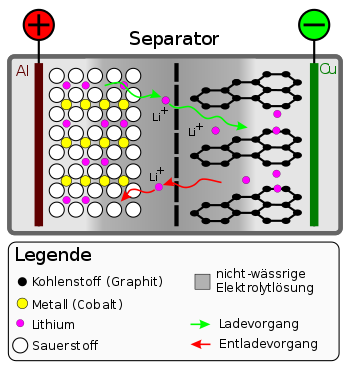
\includegraphics[scale=0.5]{figures/Akku/350px-Li-Ion-Zelle_(CoO2-Carbon,_Schema).svg.png}
		\caption{Grundaufbau einer Lithium-Ionen Zelle \cite{GrundaufbauLiionenZelle}}
		\label{fig:Grundaufbau einer Lithium-Ionen Zelle}
	\end{center}
\end{figure}
\newpage

\subsubsection{Lagerung und Sicherheithinweise}
Auch wenn Lithium nur als Li-Verbindungen in Lithium-Ionen Akkumulatoren vorhanden sind, sind die Komponenten eines solchen Akkus extrem leicht entzündbar, da Lithium ein hochreaktives Metall ist. Beim Überladen sind Ausgleichsreaktionen (z.B. die Zersetzung von Wasser), bei Lithium-Ionen Akkus nicht möglich, wie bei anderen Akkumulatoren dies der Fall ist. Schutzschaltungen die intern verbaut sein sollten, müssen eine solche Verpuffung verhindern. Andernfalls wird sonst die Funktionsfähigkeit des Akkus zerstört und er wird unbrauchbar. 
Jedoch kann es nicht nur zu inneren Beschädigungen kommen. Im Falle von inneren Kurzschlüssen, kann es passieren, dass mechanische Beschädigungen entstehen. Der hohe Kurzschlussstrom lässt zum Beispiel das Gehäuse schmelzen oder sogar in Flammen aufgehen. Es kann auch passieren, dass man den Defekt nicht unmittelbar erkennen kann. Doch kurze Zeit später kann es bereits zum Ausbruch eines Feuers kommen\footnote{vgl. \cite{LithiumIonenAkkumulatorLagerung}}.

\textbf{Lagerung:}

Im Idealfall, sollten Lithium Ionen Akkus bei einem Ladezustand zwischen 40 - 60 Prozent kühl aufbewahrt und gelagert werden.


\textbf{Sicherheitshinweise:}

\begin{itemize}
	\item{Es ist wichtig, dass Lithium-Ionen Akkus nur mit passenden Ladegeräten aufgeladen werden. Schnell-Ladegeräte für Lithium Akkumulatoren können beispielsweise eingesetzt werden. Man muss darauf achten, dass sie immer unter Aufsicht und möglichst nicht in der Nähe von brennbaren Materialien benutzt werden.} \medskip\\

	\item {Lithium-Ionen Akkus sind zwar hermetisch gekapselt, dennoch sollten sie unter keinen Umständen in Wasser getaucht werden. Besonders defekte und  vollgeladene Lithium-Zellen reagieren meist heftig mit Wasser.}\medskip\\
	
	\item {Lithium-Ionen Akkumulatoren sind mechanisch sehr empfindlich. Durch einen internen Kurzschluss und einem Kontakt mit Luft können sie sich schnell entzünden.}\medskip\\
	
	\item {Eine Lithium-Ionen Zelle die in Flammen steht, wenn möglich mit Sand und nicht mit Wasser löschen, da dies zu einer heftigen Reaktion führen kann.}\medskip\\
	
	\item {Lithium-Zellen sollten niemals über 4,2V geladen und nicht unter 2,5V pro Zelle entladen werden. Außerdem dürfen Zellen niemals kurzgeschlossen werden. Bei einem Ladevorgang ist auf eine gute Wärmeabfuhr zu achten (nicht in die Sonne legen).}\medskip\\
	
	\item {Mehrere Lithium-Zellen sollten nur dann gleichzeitig geladen werden, wenn eine Schutzschaltung vorhanden ist.}\medskip\\
	
	\item {Die Elektrolytflüssigkeit ist brennbar. Sollte aus einer Zelle Elektrolytflüssigkeit austreten, diese am besten sofort zu entsorgen.}\medskip\\
	
	\item {Man sollte versuchen die Lithium-Zellen bei einer Restkapazität von 20 Prozent nachzuladen.}\medskip\\

\end{itemize}
\newpage

\subsubsection{Anwendungsbereiche von Lithium-Ionen Akkumulatoren}
Lithium-Ionen Akkus versorgten anfangs hauptsächlich tragbare Geräte mit hohem Energiebedarf, für die herkömmliche Nickel-Cadmium- oder Nickel-Metallhydrid Akkus zu schwer oder zu groß waren, beispielsweise Mobiltelefone, Tabletts, Digitalkameras, Camcorder, Notebooks, Handheld-Konsolen oder Taschenlampen. In der heutigen Zeit sind Lithium-Ionen Akkumulatoren fast in allen denkbaren Bereichen aufzufinden. In der Elektromobiliätsbranche dienen sie oftmals als Energiespeicher für Elektroautos, moderne elektronisch betriebene Rollstühle und auch für Hybridfahrzeuge. Auch im Modellbau haben sie schon früh Verwendung gefunden. Dadurch, dass Lithium Akkus ein deutlich geringeres Gewicht als andere Batteriearten aufweisen, sind sie in Verbindung mit bürstenlosen Gleichstrommotoren und den entsprechenden Reglern, gut als Antriebseinheit im Flugmodellbau geeignet. Schon seit Anfang des 21. Jahrhunderts, gibt es Lithium-Ionen Akkus auch in Elektrowerkzeugen wie zum Beispiel Akkuschraubern. Auch im Flugbetrieb haben diese Batterien Verwendung gefunden. In der Boeing 787 werden ebenfalls Lithium-Kobaltoxid-Akkus (LiCoO2) verwendet. Zum Großen Teil werden Lithium-Ionen-Batterie-Systeme auch in Batterie-Speicherkraftwerken und Solarbatterien eingesetzt.
\newpage


\subsection{Batteriemanagementsystem}
\label{Batteriemanagementsystem}
Batteriemanagementsysteme (BMS) sind elektronische Regelschaltungen, die Akkumulatoren oder Akkupacks auf Ladung und Entladung überwachen und ebenfalls regeln. Die Batteriekennwerte die man überwachen kann bzw. möchte, hängen oftmals von dem Projekt ab. Zu den häufigsten Batteriekennwerten gehören die Erkennung des Batterietyps, die Batteriespannung, die Spannung sowie die Temperatur einzelner Batteriezellen, die Akkukapazität, der Ladezustand, die Restbetriebszeit, die Stromentnahme und einige Kennwerte mehr. Die Hauptaufgabe von BMS-Systemen besteht darin, sicherzustellen, dass die Restenergie in einer Zelle optimal genutzt wird. Um keine Beschädigungen an Zellen zu bekommen, schützt das Batteriemanagementsystem die Batterien vor Tiefenentladung, vor Überspannung, vor zu schneller Ladung (begrenzen des Ladestroms) und ebenfalls vor einem zu hohen Entladestrom. Bei Akkupacks, d.h. Akkumulatoren mit mehreren Zellen, sorgt das Batteriemanagementsystem außerdem für ein sogenanntes Balancing, das sich darin ausdrückt, dass die verschiedenen Batteriezellen gleiche Ladezustände und Entladezustände haben\footnote{vgl. \cite{Batteriemanagementsystem}}.

\begin{figure}[H]
	\begin{center}
		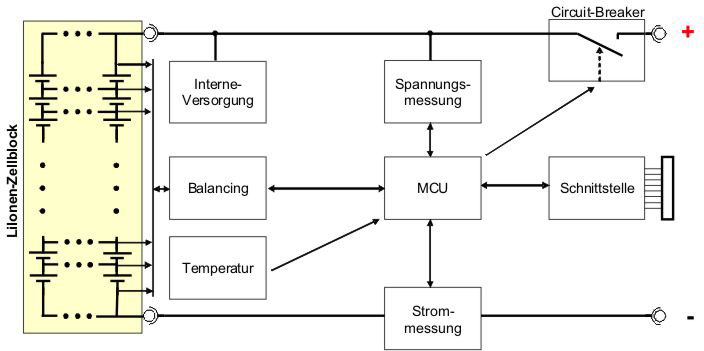
\includegraphics[scale=0.5]{figures/Akku/bms-1schaltunggrund.jpg}
		\caption{Grundschaltung eines Batteriemanagementsystems\cite{GrundschaltungBMS}}
		\label{Grundschaltung eines Batteriemanagementsystems}
	\end{center}
\end{figure}

Grundsätzlich setzt sich ein vollständiges Batteriemanagementsystem aus folgenden Komponenten zusammen:
\begin{itemize}
	\item \textbf{Cell Supervising Circuit(CSC):} \medskip\\
	Die Aufgabe des CSC besteht darin die Zellen auf Spannung und 			Temperatur zu überwachen.

	\item \textbf{Kontrolleinheit:}\medskip\\
	Die Kontrolleinheit berechnet die State of Charge (SOC), die State 	of Health (SOH) und überprüft auch die Funktionalität der 				Batterien (State of Function). Außerdem wird von der 					Kontrolleinheit auch der Ladeausgleich gesteuert und kommuniziert 		über eine Serielle Schnittstelle mit einem Prozessor. 

	\item \textbf{Circuit Breaker:}\medskip\\
	Der Circuit Breaker trennt im Fehlerfall die Batterie von der 		Last. Dies erfolgt mithilfe eines HS-Kontaktors.
	
	\item \textbf{Strommessvorrichtung:}\medskip\\
	Diese Komponente ist für die Messung des Stromes zuständig.
	
	\item \textbf{Temperaturüberwachung:}\medskip\\
	Diese Komponente überprüft, ob sich die Batterien oder die 				Akkupacks in einem zulässigen Temperaturbereich befinden.
\end{itemize}
\newpage

\subsubsection{Komponenten eines BMS}

\textbf{Cell Supervising Circuit (CSC):}
Die erste Komponente eines Batteriemanagementsystem ist für die Spannungs- und Temperaturüberwachung der einzelnen Zellen zuständig und wird als Cell Supervising Circuit (CSC) bezeichnet. Ein Akkusystem besteht immer aus mindestens 2 einzelnen Zellen, oftmals jedoch aus mehreren. Deswegen ist die Spannungs- und Temperaturüberwachung jeder einzelnen Zelle nicht möglich. Es kommt  durchaus vor, dass mehrere einzelne Zellen zu sogenannten Akkupacks zusammengeschraubt oder zusammengeschweißt werden. Man hat dann wiederum die Möglichkeit, jedes Akkupack für sich mithilfe eines CSC zu überwachen.

\textbf{Kontrolleinheit:}
Die nächste Komponente wird auch als Kontrolleinheit bezeichnet. Die Aufgabe dieser Komponente liegt darin, die SOC (State of Charge) und auch die SOH (State of Health) zu berechnen. Außerdem steuert die Kontrolleinheit auch den Ladeausgleich der einzelnen Zellen oder der Akkupacks. Diese Komponente übernimmt auch die Kommunikation des Batteriemanagementsystems mit anderen angeschlossenen Einheiten. Diese Kommunikation erfolgt über eine serielle Schnittstelle wie den I2C-Bus oder dem CAN-Bus. Die Werte (SOC und SOH) und auch die SOF (State of Function) werden dann an einen Prozessor übermittel auf dem die BMS-Software läuft und außerdem der SOC-Algorithmus implementiert ist. Die Kontrolleinheit ist fähig sich selbst in einen Ruhezustand zu versetzen um den eigenen Stromverbrauch um ein Minimum zu reduzieren.

\begin{itemize}
	\item \textbf{State of Health (SOH):} \medskip\\
	Beschreibt den aktuellen Alterungszustand der Batterie. Ein Kriterium dafür ist, welche Ladungsmengen die Zellen noch aufnehmen. Je älter die Akkumulatoren werden, desto weniger Aufnahmevermögen haben sie.

\item \textbf{State of Charge (SOC):} \medskip\\
	Beschreibt den momentanen Ladezustand der Batterie. Außerdem gibt er Auskunft darüber, wie viel beziehungsweise wie lange die Batterie noch Energie bereitstellt. Beim Aufladen der Akkus gibt es an, wie viel Energie er noch aufnehmen kann.

\item \textbf{State of Function (SOF):} \medskip\\
	Gibt die Funktionalität der Batterie an. State of Function beschreibt die Leistungsfähigkeit der Batterie. Also wie viel kW der Energiespeicher dem Motor zum Beispiel bereitstellen kann. Die Leistungsfähigkeit lässt mit zunehmendem Batteriealter nach.
\end{itemize}

\textbf{Circuit-Breaker:}
Tritt ein Fehler bei einer einzelnen Zelle oder auch einem ganzen Akkupack auf, wird diese Batterie mithilfe eines HS-Kontaktors (Circuit-Breaker) von der Last getrennt. Dies schützt den Akkumulator. Dieser Kontaktor übernimmt außerdem noch die Trennung eines Akkumulatoren im Ruhezustand. Fehler die durch Trennen der Last beseitigt werden können sind zum Beispiel Kurzschlüsse oder auch Übertemperatur. Für den Kurzschlussfall sind meisten auch noch Schmelzsicherungen (eine Art Sollbruchstelle im Stromkreis; die Wärmewirkung des Stromes wird ausgenutzt) verbaut die verhindern, dass Leitungen oder auch das Gehäuse in Flammen aufgehen.

\textbf{Strommessvorrichtung:}
Diese Komponente ist wie der Name schon beschreibt, für die Messung des Stromes zuständig. Oftmals werden dazu zwei voneinander unabhängige Systeme verwendet. Um den Strom messen zu können, wird ein Messsensor verwendet. Dies ist meist ein einfacher Widerstand. Bei der zweiten Methode wird der Strom über das elektromagnetische Feld gemessen.

\textbf{Temperaturüberwachung:}
Die letzte Komponente, die benötigt wird, um das Batteriemanagementsystem zu vervollständigen, ist für den Temperaturausgleich zuständig. Das heißt, es wird überwacht ob sich der Akkumulator in einem zulässigen Temperaturbereich findet. Sollte das nicht der Fall sein, können innere sowie auch äußere Schäden an der Batterie entstehen. Außerdem wirkt sich die Temperatur auf die Lebensdauer der Akkus auf.
\newpage

\subsubsection{Battery-Balancing}
\label{Battery-Balancing}
Der Ausdruck Balancing bezogen auf Akkumulatoren bedeutet so viel wie Ladeausgleich. Ohne Battery-Balancing bestimmt in einem Mehrzellen-Akku immer die schwächste Zelle darüber, welche Kapazität oder Spannung das Gesamtsystem aufweist. Das ergibt sich daraus, da sich jede Zelle minimal von einer anderen Zelle, durch ihre chemischen Struktur, unterscheidet. Einzelne Batteriezellen können auch unterschiedlich altern und deswegen kann man nie sicherstellen, dass jede Zelle exakt die identische Kapazität aufweist. Manche Zellen laden etwas schneller oder langsamer als andere. Wiederrum andere Batterien entladen sich etwas zügiger oder eben auch langsamer. In der Regel gibt es zwei verschiedene Arten von Battery-Balancing.
\begin{itemize}
\item \textbf{Passives Battery-Balancing} \medskip\\
\item \textbf{Aktives Battery-Balancing} \medskip\\
\end{itemize}


\textbf{Akkupacks:}

"Cluster oder Akkupacks bestehen zur Erhöhung der Nennspannung in der Regel aus mehreren in Reihe geschalteten Einzelzellen oder Zellblöcken. Fertigungs- und alterungsbedingt gibt es hierbei Schwankungen in der Kapazität, im Innenwiderstand und weiteren Parametern dieser Zellen. Die schwächste Zelle ist dabei bestimmend, wie viel geladen oder entladen werden darf. Im praktischen Einsatz von mehrzelligen in Reihe geschalteten Akkus führt dieser Umstand dazu, dass die Zellen in Reihe unterschiedlich geladen und entladen werden.

Es kommt dann im Verbund zu kritischer Tiefentladung oder bei der Ladung zu einer Überladung und Überschreiten der Ladeschlussspannung einzelner Zellen. Je nach Typ kann es dabei zu einer irreversiblen Schädigung einzelner Zellen kommen. Die Folge: das gesamte Akkupack verliert an Kapazität".\footnote{Quelle des Zitat: \cite{BalancingderPacks}}
Um das zu verhindern, spielen im Batteriemanagementsystem die Balancer eine wichtige Rolle.

\newpage

\fancyfoot[C]{Lackner}

\section{Synchronmaschine mit Dauermagneterregung}
\subsection{Allgemeines}
Die permanenterregte Synchronmaschine benötigt keine zusätzlichen Komponenten für die Einspeisung des Erregersystems. Neben dem Wegfall der Schleifringe bzw. des Kommutators hat die PSM noch weitere Vorteile:
\\[5mm]
\begin{itemize}
	\item Aufgrund der Erregung mit Permanentmagneten ist die Einspeisung einer flussbildenden Blindstromkomponente, wie bei der Asynchronmaschine bekannt ist, nicht notwendig. Somit ist der einzuspeisende Strom und damit der Energieverbrauch für vergleichbare Maschinen kleiner\footnote{vgl. \cite{Dissertation}, S. 15ff.}. \\[3mm]
	\item Weiters erlauben die fehlende Läufernutung und die hohe Remanenzflussdichte der Dauermagneten höhere Luftspaltflussdichten, dadurch lassen sich auch höhere Leistungsdaten realisieren. \\[3mm]
\end{itemize}

Verglichen mit Asynchronmaschinen haben permanenterregte Synchronmotoren also eine mindestens doppelt so große Bemessungsleistung bei gleicher Baugröße, zudem besitzen sie ebenfalls weniger Gesamtverluste. Die PSM müssen jedoch anwendungsspezifischer ausgelegt werden, denn es entfallen alle Einflussmöglichkeiten auf die Betriebsdaten, speziell auf Betrag und Phasenlage des Ständerstroms, die sonst durch die Änderung des Feldes über den Erregerstrom gegeben sind.

\subsection{Aufbau}
Um eine gute Ausnutzung des Bauvolumens realisieren zu können, wird der Ständer meist mit einer sechspoligen Drehstromwicklung ausgeführt. Der Läufer ist dabei wie in folgender Abbildung beschrieben mit Dauermagneten ausgeführt. Große Aussparungen im Läuferblech (2) reduzieren das Trägheitsmoment und führen zu besseren dynamischen Eigenschaften\footnote{vgl. \cite{Fischer}, S. 348ff; S. 405}.
\\[3mm]
\begin{figure}[H]
	\begin{center}
		\includegraphics[scale=0.7]{figures/antrieb/Läufer_Synchronmaschine.jpg}
		\caption{Läufer einer dauermagneterregten Synchronmaschine \cite{Fischer}}
	\end{center}
\end{figure}

\subsection{Funktionsweise}
Im Motorbetrieb wird an die Klemmen der Ständerwicklungen ein Drehstrom angelegt und dadurch ein sinusförmiges Drehfeld erzeugt. Da sich ungleiche magnetische Pole anziehen, wird der Rotor mit seinem zugehörigen Magnetfeld synchron mit dem angelegten Drehfeld mitbewegt. Im Leerlauf stehen sich also der Nordpol des Stator-Drehfelds und der Südpol des permanenterregten Rotor-Magnetfelds exakt gegenüber, die Drehzahl des Läufers ist also synchron mit der Drehzahl des angelegten Drehfelds. Bei bremsender Last eilt das Magnetfeld des Permanentmagneten dem Stator-Drehfeld um den Polradwinkel nach. Die Größe des Winkels stellt sich also abhängig von der Stärke des Lastdrehmoments ein. Dies kann jedoch nur bis zum sogenannten Kippmoment (Polradwinkel $\vartheta = 90^\circ$) gesteigert werden. Übersteigt das Drehmoment der Last das Kippmoment, so spricht man vom \glqq Abreißen\grqq{} der magnetischen Felder und die Synchronmaschine bleibt stehen. Das selbe gilt für den Generatorbetrieb, hier eilt aber das Drehfeld des Rotors vor. Bei Frequenzumrichterspeisung mit Feldorientierung kann jedoch dauerhaft mit $\vartheta$ = +/- $90^\circ$ gefahren werden, man spricht von sogenannter Querstromspeisung, der Zusammenhang zwischen (Läufer)-Feld und (Ständer)-Strom entspricht dann jenem der fremderregten Gleichstrommaschine\footnote{vgl. \cite{Synchronmaschine}}.

	
\newpage

\subsection{Auswertung der Antriebswelle (Encoder)}
Für den Betrieb einer permanentmagneterregten Synchronmaschine wird immer ein zugehöriger Frequenzumrichter benötigt. Um eine gute Regelung einer Synchronmaschine gewährleisten zu können, benötigt dieser die Rückmeldung von einem Resolver (Encoder) oder einem hochauflösenden Inkrementalgeber, welcher im Motorgehäuse integriert ist. Denn im Betrieb mit sinusförmigen Strömen muss die exakte Läuferfeldlage bekannt sein, um eine feldorientierte Regelung durchführen zu können\footnote{vgl. \cite{Fischer}, S. 405.} .

Die Übertragung des elektrischen Signals erfolgt in Synchronmaschinen mit eingebauten Dauermagneten am häufigsten mit einem Sinus/Cosinus-Sensor. Der Sensor besteht hierbei aus zwei Versorgungsleitungen (positive Spannungsversorgung = 5V; Ground = 0V) und zwei Sensordrähten. Über die zwei Sensordrähte wird das Spannungssignal (0-5V) abhängig vom aktuellen Stand der Motorwelle ausgegeben. Betrachtet man die Spannungswerte über den gesamten Winkel der Motorwelle, erkennt man zwei sinusförmige Kurven, die um $90^\circ$ versetzt sind. Bei einer korrekten Auswertung dieser Signale kann der aktuelle Stand der Motorwelle in jeder beliebigen Position absolut bestimmt werden.
\\[8mm]
\begin{figure}[H]
	\begin{center}
		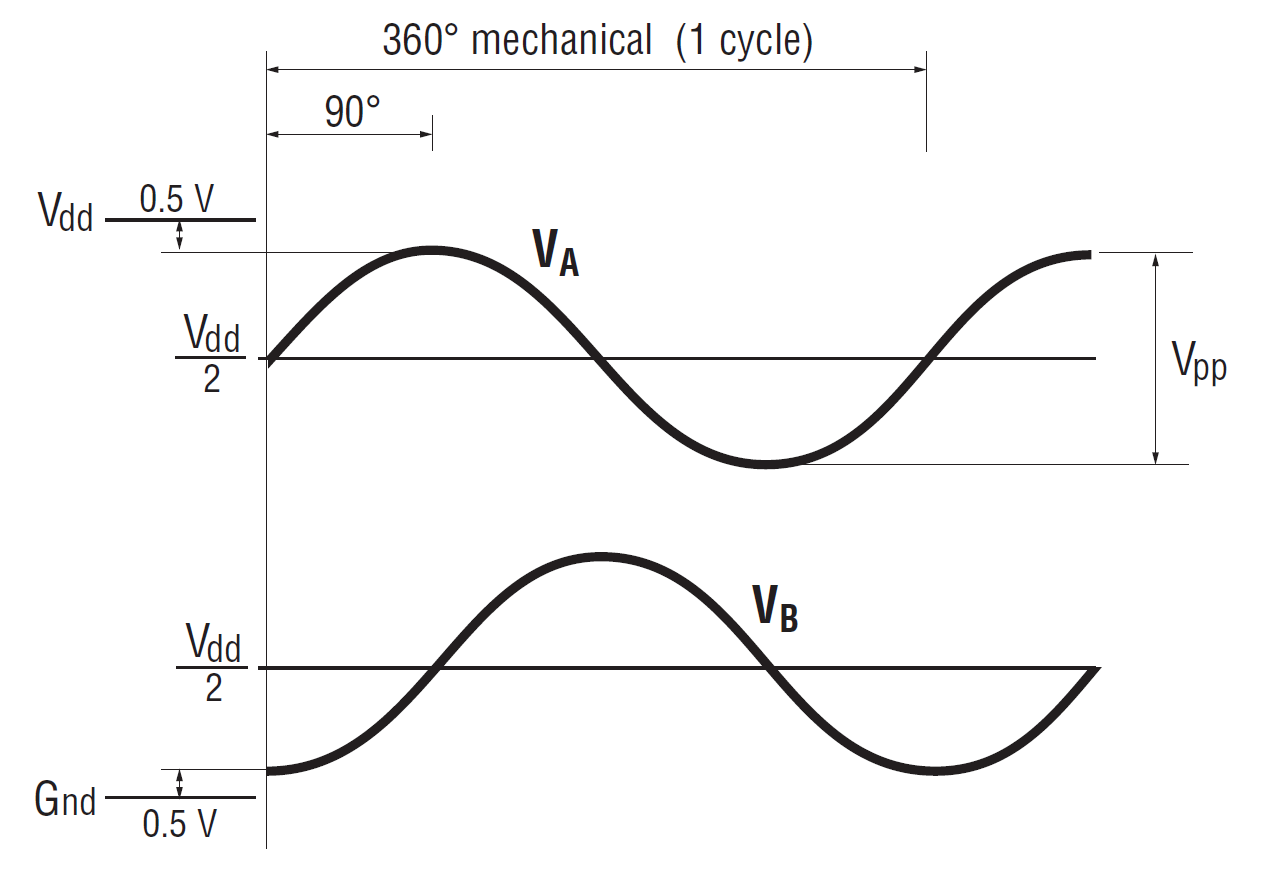
\includegraphics[scale=0.3]{figures/antrieb/SinCos_Sensor.png}
		\caption{Ausgabe eines Sinus/Cosinus-Sensors \cite{Manual}}
	\end{center}
\end{figure}



\newpage

\section{Curtis Controller}
\subsection{Allgemeines}
Der Curtis Controller ermöglicht eine genaue, zuverlässige und hocheffiziente Regelung von Drehzahl und Drehmoment bei Wechselstrom-Induktionsmotoren (ACIM) und Permanentmagnet-Synchronmotoren (PSM). Dieser Motorcontroller verfügt über zwei unabhängige Mikroprozessoren, um gleichzeitig eine außergewöhnliche Leistungsfähigkeit und funktionale Sicherheit gewährleisten zu können. 

Der primäre Mikroprozessor führt eine fortschrittliche feldorientierte AC-Motorregelung durch, ebenso beinhaltet er einen weiteren integrierten Logik-Prozessor für eine zeitgleiche Operation durch die VCL-Software. Der zweite Mikroprozessor überwacht kontinuierlich den Betrieb des Gesamtsystems. Er misst Eingänge und kontrolliert die zugehörigen Ergebnisse, weiters überprüft er kritische Zeitpunkte und Operationen. 

Die Vehicle-Control-Language (VCL) ist eine  innovative Programmiersprache, welche von Curtis entwickelt wurde. Sehr viele einzigartige Funktionen sind in dieser Programmiersprache enthalten, weiters können bei Bedarf selbst Funktionen erstellt und konfiguriert werden. VCL eröffnet neue Möglichkeiten der Anpassung, sodass bestimmte fahrzeugspezifische Anwendungen schnell und einfach in der Motorsteuerung selbst erstellt werden können, um den Einbau von zusätzlichen Steuer-Modulen verhindern zu können.

Für die umfassende Einsatzmöglichkeit dieses Controllers sind ebenfalls sehr wichtige Kommunikationsmöglichkeit über den CAN-Bus gegeben. Ein- und Ausgänge können im gesamten System geteilt und optimal gemeinsam genutzt werden, wodurch die Verkabelung minimiert und zusätzliche Applikationsmöglichkeiten erstellt werden können, die häufig die Kosten des Gesamtsystems senken.

Dieser Motorcontroller ist eine ideale Lösung für Motorantriebe in der Anwendung für Elektrofahrzeuge, Hebevorrichtungen und Doppelmotorantriebe\footnote{vgl. \cite{Manual}, S. 1.}.
\\[10mm]
\begin{figure}[H]
	\begin{center}
		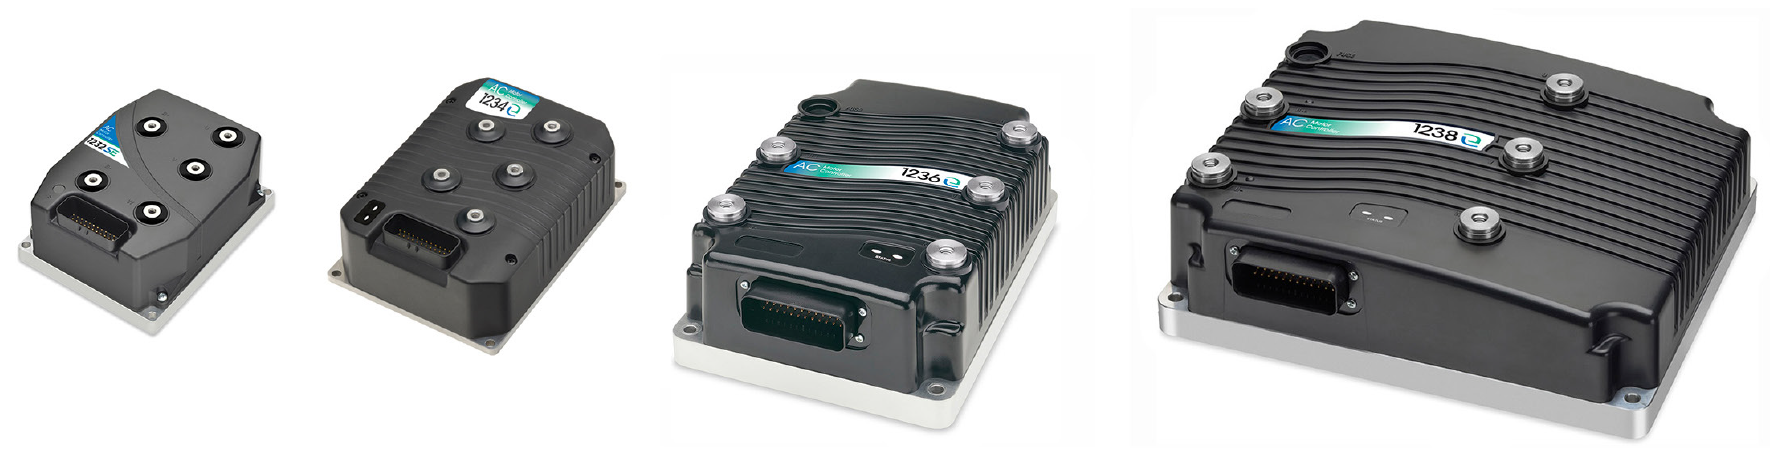
\includegraphics[width=\textwidth]{figures/antrieb/Curtis_Bauformen.png}
		\caption{Übersicht der häufigsten Bauformen eines Curtis Controllers \cite{Manual}}
	\end{center}
\end{figure}



\newpage
 
\subsection{Feldorientierte Regelung}
"Die herkömmliche Technik zur Regelung von PSM wird als Sechsstufen- oder Trapezsteuerung bezeichnet. Dabei wir der Stator in einem sechsstufigen Prozess angesteuert, der Schwankungen des erzeugten Drehmoments hervorruft. Jedes Wicklungspaar wird einzeln erregt, bis der Rotor die nächste Position erreicht, dann wird der Motor zum nächsten Schritt kommutiert. Skalare Techniken sind jedoch für Anwendungen mit dynamisch wechselnden Lasten nicht präzise genug". Durch den Einsatz der feldorientierten Regelung lässt sich die Präzision, Effizienz und Lebensdauer des Antriebs erheblich steigern, weiters lassen sich bei hohen und niedrigen Drehzahlen leistungsstarke Drehmomentregelungen realisieren\footnote{vgl. \cite{Feldorientierte-Regelung}}.

Die feldorientierte Regelung (auch Vektorregelung genannt) ist ein sinusförmiges Kommutierungsverfahren. Der Motorcontroller hat die Aufgabe die Statorströme zu berechnen, um den Rotor basierend auf der Stromrückkoppelung des Motors ansteuern zu können. Abgeleitet von der Raumzeigerdarstellung für Wechselspannungen und -strömen und deren Bezug zueinander wird ein rotierendes Koordinatensystem mit den Größen Drehmoment und magnetische Flussdichte als Achsen erstellt. Das Verfahren wandelt die Statorströme über dieses Koordinatensystem in magnetische Flussdichte und Drehmoment erzeugende Komponenten um. Zudem regelt es die Statorströme über einen PID-Regler und wandelt sie dann in drei Spannungswerte zurück, aus denen wiederum der PWM-Ausgang erstellt wird. Dieser ist dann auch für das sinusförmige Kommutierungssignal verantwortlich\footnote{vgl. \cite{Feldorientierte-Antriebssteuerung}}.
\\[7mm]
\begin{figure}[H]
	\begin{center}
		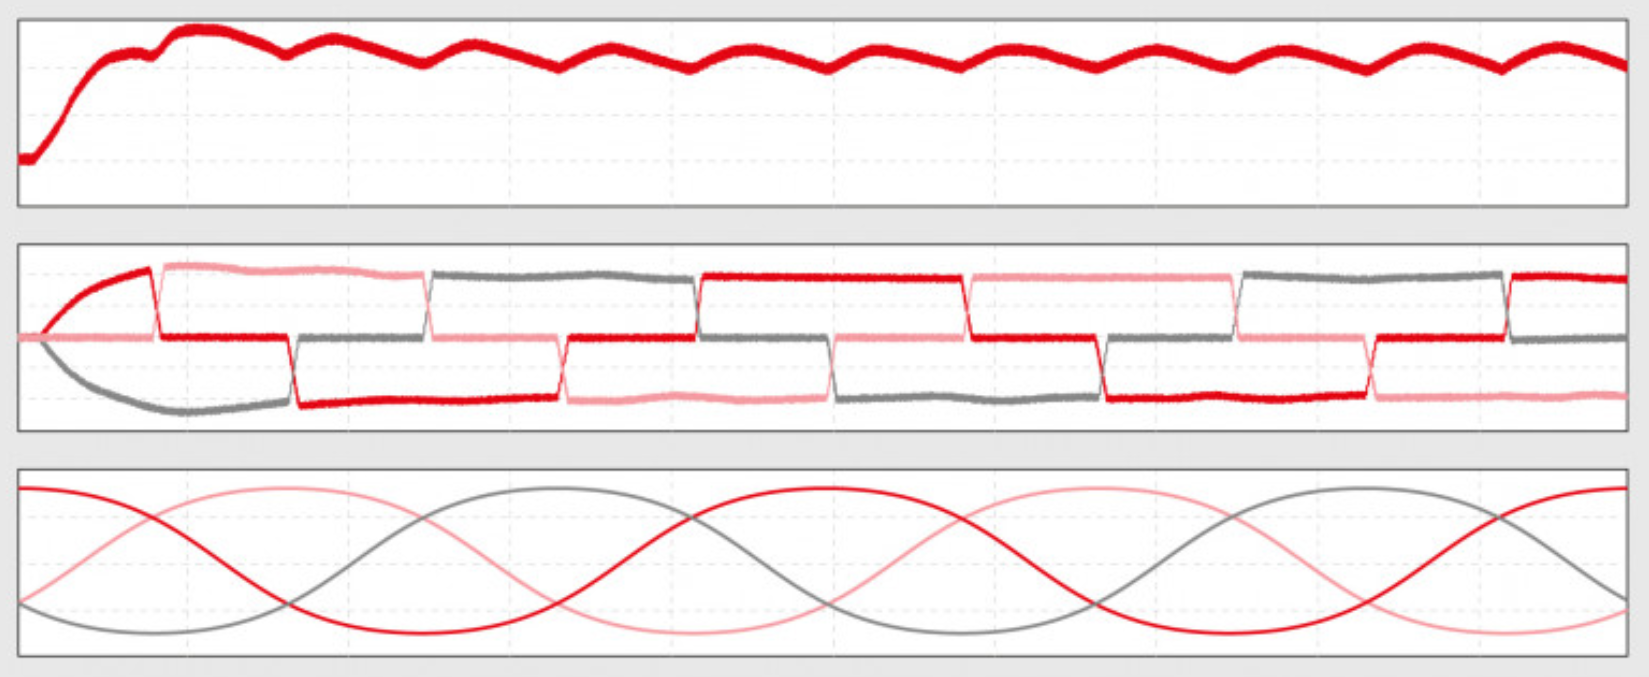
\includegraphics[width=0.9\textwidth]{figures/antrieb/Kommutierung_Trapezsteuerung.png}
		\caption{Kommutierung mittels Trapezsteuerung \cite{Feldorientierte-Antriebssteuerung}}
	\end{center}
\end{figure}

\begin{figure}[H]
	\begin{center}
		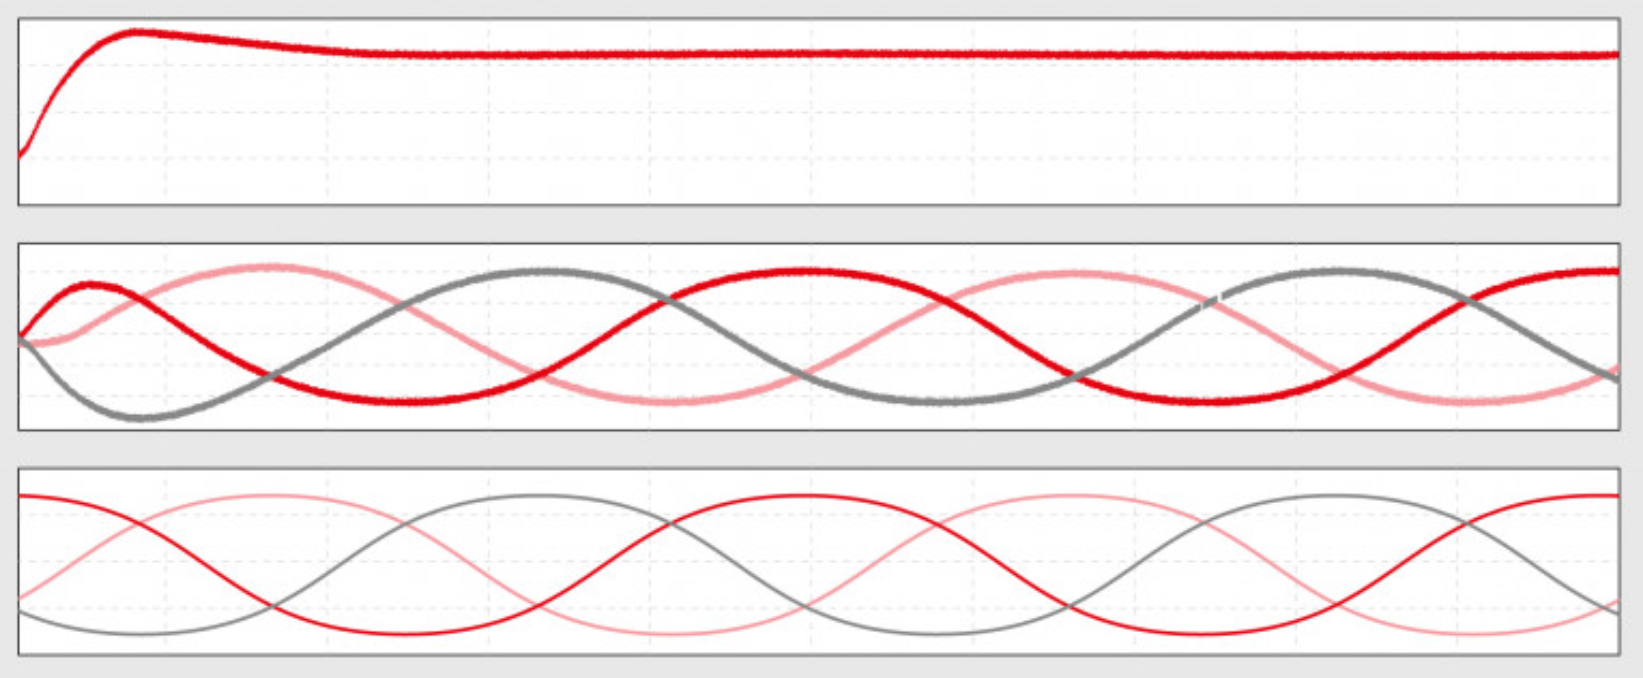
\includegraphics[width=0.9\textwidth]{figures/antrieb/Kommutierung_Vektorregelung.png}
		\caption{Kommutierung mittels Vektorregelung \cite{Feldorientierte-Antriebssteuerung}}
	\end{center}
\end{figure}

%https://www.digikey.de/de/articles/field-oriented-control-of-small-dc-motors-put-drones-on-a-rising-flight-path
%https://www.all-electronics.de/foc-mcu-antriebssteuerung/

\newpage



\section{Der Regler}
\subsection{Einleitung}
"Regelungen sind ein Bestandteil unseres Lebens und das nicht nur seit Erfindung der Dampfmaschine.

Allein schon der aufrechte Gang funktioniert nur mit Regelung. Dabei wirken die Sinne als Sensoren, das Gehirn als Regler und die Muskeln als Aktoren. Weitere Regelungen in unserem Körper sind z.B. die Konstanthaltung der Körpertemperatur, der Blutdruck, die Anpassung der Pupille auf Helligkeitsänderungen usw.

Der Begriff Regelung ist zu unterscheiden von dem im allgemeinen Sprachgebrauch oft synonym gebrauchten Begriff der Steuerung. Das Steuern ist ein rein vorwärts gerichteter Prozess ohne Rückkopplung. Die Ausgangsgröße wird dabei nicht überwacht und kann sich durch Störungen von außen verändern. Ein Beispiel ist die Steuerung eines Elektromotors mit einer einstellbaren Spannung. Durch Laständerungen wird sich die Drehzahl des Motors ändern. Soll nun die Drehzahl konstant gehalten werden, bedarf es einer Rückkopplung, um über die Spannung die Drehzahl anzupassen. Diese Rückkopplung ist das Kennzeichen einer Regelung.

Das Regeln ist ein Vorgang, bei dem die Ausgangsgröße, im Beispiel die Drehzahl, fortlaufend überwacht wird und bei Abweichung über die Stellgröße, im Beispiel die Spannung, korrigiert wird. Der sich dabei ergebende Wirkungsablauf findet in einem geschlossenen Kreis, dem Regelkreis, statt.
\vspace{5mm}

\subsection{Der Regelkreis}
Das Prinzip einer Regelung ist das fortlaufende Messen – Vergleichen – Stellen.
\\[5mm]

\begin{itemize}
	\item \textbf{Messen}
	\\[1mm] Die Regelgröße wird mittels Sensoren gemessen.
	\medskip
	\item \textbf{Vergleichen}
	\\[1mm] Der Wert der Regelgröße wird mit dem Sollwert verglichen. Die Differenz ist die Regelabweichung.
	\medskip
	\item \textbf{Stellen}
	\\[1mm] Aus der Regelabweichung wird unter Berücksichtigung der dynamischen Eigenschaften der Regelstrecke die Stellgröße bestimmt.
\end{itemize}
\vspace{3mm}

Ein Regelkreis dient dazu, eine vorgegebene physikalische Größe, die Regelgröße, auf einen gewünschten Wert (Sollwert) zu bringen und dort zu halten, unabhängig von eventuell auftretenden Störungen. Um die Regelungsaufgabe zu erfüllen, muss der Augenblickswert der Regelgröße – der Istwert – gemessen und mit dem Sollwert verglichen werden. Auftretende Abweichungen müssen in geeigneter Art und Weise nachgestellt werden.

Um nun diese Aufgabe technisch zu lösen, gibt es die Regelungstechnik. Sie baut im wesentlichen auf die mathematische Beschreibung und Modellbildung des Systems Regelkreis. Zur Modellierung, Beschreibung und Simulation werden Blockschaltbilder mit diskreten Signalgliedern verwendet".\footnote{Zitatquelle: \cite{Regelungstechnik}}
	
\newpage

Ein Regelkreis besteht entsprechend des vereinfachten Blockschaltbildes, wie es meist in der Regelungstechnik verwendet wird, aus den Hauptteilen Regler und Regelstrecke:
\\[5mm]

\begin{itemize}
	\item \textbf{Regler G$_R$}
	\\[1mm] Um die Regelabweichung zu minimieren müssen Korrekturmaßnahmen ergriffen werden.
	\medskip
	\item \textbf{Regelstrecke G$_S$}
	\\[1mm] Das zu regelnde System \medskip
	\item \textbf{Führungsgröße w (Sollwert)}
	\\[1mm] Vorgegebener Wert, auf dem die Regelgröße durch die Regelung gehalten werden soll. \medskip
	\item \textbf{Regelgröße x (Istwert)}
	\\[1mm] Die Ausgangsgröße der Regelstrecke wird für den Vergleich mit dem Sollwert bzw. zur Berechnung der Regelabweichung rückgekoppelt. \medskip
	\item \textbf{Regelabweichung e}
	\\[1mm] Differenz zwischen Führungsgröße und Regelgröße e = w – x, bildet die eigentliche Eingangsgröße des Reglers. \medskip
	\item \textbf{Stellgröße y}
	\\[1mm] Die Ausgangsgröße des Reglers wird vom zu regelnden System beeinflusst. \medskip
	\item \textbf{Störgröße z}
	\\[1mm] Es können unvorhersehbare Störgrößen auftreten, die ebenfalls ausgeregelt werden müssen.
\end{itemize}

\vspace{7mm}
\begin{figure}[H]
	\begin{center}
		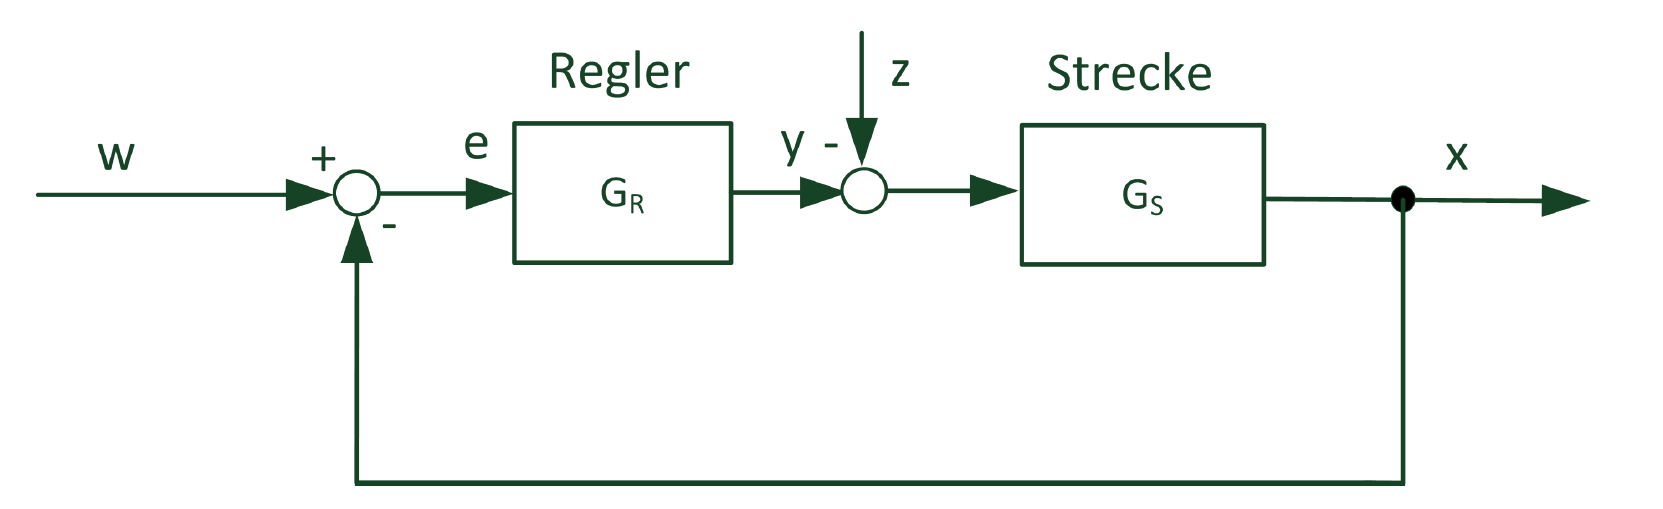
\includegraphics[width=\textwidth]{figures/antrieb/Regelkreis_Grundaufbau.png}
		\caption{Das Blockschaltbild eines allgemeinen Regelkreises \cite{AUT5}}
	\end{center}
\end{figure}

\newpage

\subsection{Der PID-Regler}
Der PID-Regler vereint die guten Eigenschaften der anderen klassischen Regler. Der PID-Regler ist genau und sehr schnell, in den meisten Anwendungen kann dieser Regler deshalb verwendet werden. Vorab sollte man jedoch überprüfen, ob ein einfacherer bzw. billigerer Regler für die Realisierung der gewünschten Anwendung ebenfalls ausreicht.
\\[5mm]
Der PID-Regler besteht grundlegend aus drei einzelnen Reglern, die mit einander kombiniert werden:
\\[5mm]
\textbf{P-Anteil}\\[1mm]
Der proportionalwirkende Regler multipliziert die Regelabweichung mit seinem Verstärkungsfaktor Kp und gibt das Ergebnis unverzögert weiter. Der P-geregelte Kreis ist einfach und mittelschnell im Vergleich zu anderen Regelungen. Das Problem hierbei ist die bleibende Regelabweichung!
\\[4mm]
Reglergleichung: \hspace{5mm} $y(t) = K_P \cdot e(t)$ \hspace{5mm} bzw. \hspace{5mm} G$_R$ = K$_P$
\\[7mm]

\textbf{I-Anteil}\\[1mm]
Der integralwirkende Regler summiert die Regelabweichung über der Zeit auf und multipliziert die Summe (d.h. das Integral) mit dem Faktor Ki. Je länger eine Regelabweichung ansteht, desto größer wird die Stellgröße des I-Reglers. Der I-geregelte Kreis ist langsam im Vergleich zu anderen Regelungen. Er hat aber den Vorteil, dass die Abweichung vollständig eliminiert wird.
\\[4mm]
Reglergleichung: \hspace{5mm} $y(t) = K_I \cdot \int\limits_{0}^{t} e(t) \,dt$ \hspace{5mm} bzw. \hspace{5mm} $G_R = \dfrac{K_I}{s}$
\\[7mm]

\textbf{D-Anteil}\\[1mm]
Der D-Anteil ist ein Differenzierer, der nur in Verbindung mit anderen Reglern eingesetzt wird. Er reagiert nicht auf die Regelabweichung, sondern nur auf deren Änderungsgeschwindigkeit. Je schneller sich das Signal ändert, desto größer ist die Ausgangsgröße, diese wird noch mit Kd multipliziert.

Ein Nachteil aller Regler mit D-Anteil kann die Unruhe im Kreis sein. Ist das Sensorsignal verrauscht, so wird dieses Rauschen durch das Differenzieren weiter verstärkt und wieder in den Kreis hineingegeben. Dadurch wird der Aktor stärker belastet. Solche Probleme können aber durch Anpassung der Regelparameter oder mit dem Hinzufügen eines Filters behoben werden\footnote{vgl. \cite{PID-Regler}},\footnote{vgl. \cite{AUT5}, Kapitel 4}.
\\[4mm]
Reglergleichung: \hspace{7mm} $y(t) = K_D \cdot \dfrac{de(t)}{dt}$\hspace{5mm} bzw. \hspace{5mm} $G_R = K_D \cdot s$

\newpage

Kombiniert man also die drei unterschiedlichen Regler miteinander, so erhält man den sogenannten PID-Regler, dieser vereint die guten Eigenschaften der einzelnen Regler. Der P-Regler ist für die schnellen Korrekturen zuständig, er reagiert ohne Verzögerung auf die Regelabweichung. Der I-Regler überwacht die Regelung des P-Reglers und korrigiert diese über die Zeit, um eventuelle Regelabweichungen auszubessern. Der D-Anteil verstärkt bei schnellen Veränderungen beide Regelkreise, um das Ansprechverhalten zu verbessern\footnote{vgl. \cite{PID-Regler}}.
\\[4mm]
Reglergleichung: \hspace{3mm} $y(t) = K_P \cdot e(t) + K_I \cdot \int\limits_{0}^{t} e(t) \,dt + K_D \cdot \dfrac{de(t)}{dt}$ \hspace{3mm} bzw. \hspace{3mm} $G_R = K_P + \dfrac{K_I}{s} + K_D \cdot s$
\\[5mm]
\begin{figure}[H]
	\begin{center}
		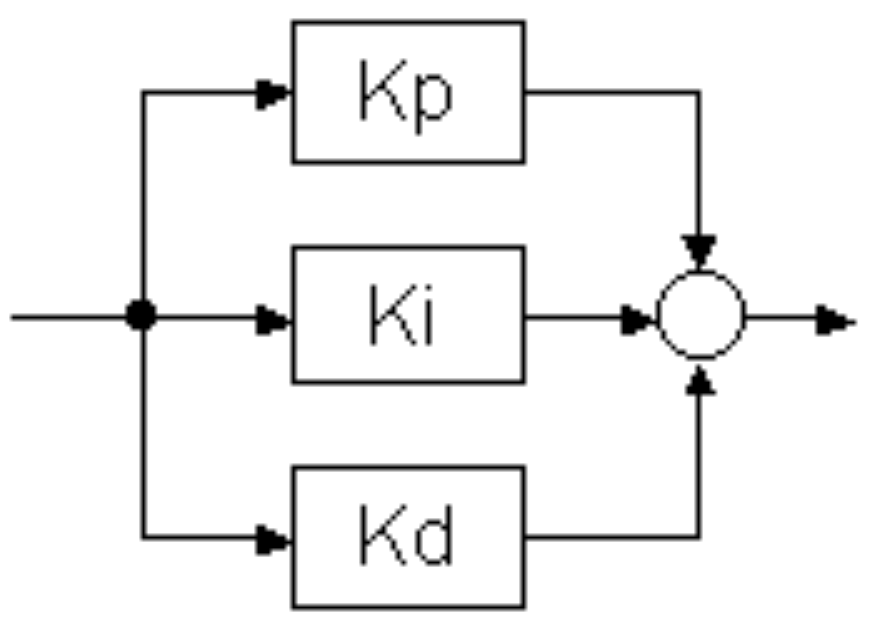
\includegraphics[scale=0.15]{figures/antrieb/PID_Regler.png}
		\caption{Zusammensetzung des PID-Reglers \cite{Regelungstechnik}}
	\end{center}
\end{figure}
\vspace{5mm}
Hier sind für ein besseres Verständnis die Sprungantworten der unterschiedlichen klassischen Reglertypen dargestellt. Der Regelkreis ist geschlossen, ein PT2-Glied bildet die Regelstrecke.
\\[4mm]
\begin{figure}[H]
	\begin{center}
		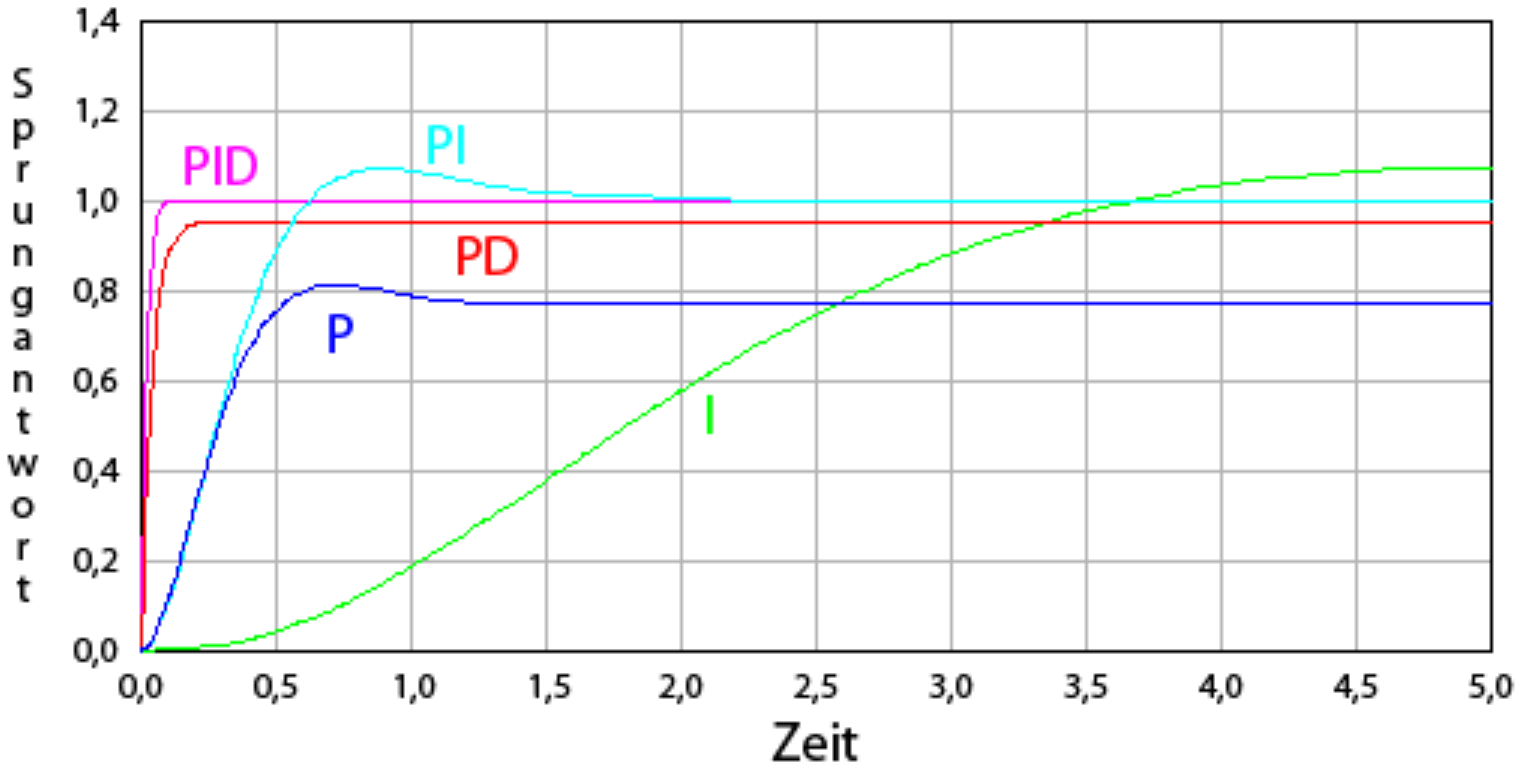
\includegraphics[scale=0.3]{figures/antrieb/Reglertypen.png}
		\caption{Vergleich der verschiedenen Reglertypen \cite{PID-Regler}}
	\end{center}
\end{figure}

%https://rn-wissen.de/wiki/index.php/Regelungstechnik
%http://3digi.wikidot.com/allgemeines-zu-pid-reglern
%AUT5
\newpage

%%%%%%%%%%%%%%%%%%% HCIS

\fancyfoot[C]{Kronberger}

\section{Bussysteme}

\subsection{CAN-Bus}

Controller Area Network ist eine serielle Netzwerktechnologie, die ursprünglich für die Automobilindustrie, insbesondere für europäische Autos, entwickelt wurde. Der CAN-Bus wird hauptsächlich in embedded systems verwendet und ist eine Netzwerktechnologie, die eine schnelle Kommunikation zwischen Mikrocontrollern bis hin zu Echtzeitanforderungen ermöglicht. \\ \medskip

CAN ist ein Zweidraht-Halbduplex-Hochgeschwindigkeitsnetzwerksystem \footnote{Halb-Duplex und Voll-Duplex bestimmen, ob Hosts Daten gleichzeitig senden und empfangen können.}, das herkömmlichen seriellen Technologien wie RS232 in Bezug auf Funktionalität und Zuverlässigkeit weit überlegen ist und dennoch sind CAN-Implementierungen kostengünstiger. \footnote{vgl. \cite{can}}

Es gibt im Gegensatz zu dem SPI-Bus hier keinen Master und Slave. Zur Übertragung wird eine Twisted-Pair Leitung mit einem positiven und einem negativen CAN-Signal (CAN-High/CAN-Low) benötigt. Parallel dazu werden die Bus-Teilnehmen (CAN-Nodes) geschalten.

\begin{figure}[H]
	\begin{center}
		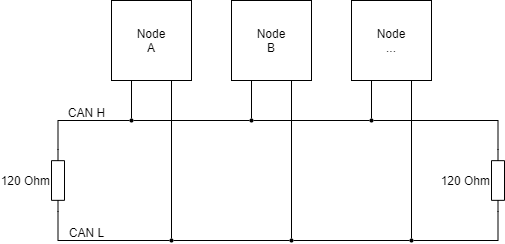
\includegraphics[scale=0.5]{figures/hcis/can_nodes.png}
		\caption{Aufbau einer CAN-Bus Leitung}
	\end{center}
\end{figure}

\subsection{SPI-Bus}

Der SPI-Bus (Serial Peripheral Interface) wurde von Motorola entwickelt, um eine synchrone serielle Vollduplex-Kommunikation zwischen Master- und Slave-Geräten zu ermöglichen. Er wird üblicherweise für die Kommunikation mit Flash-Speichern, Sensoren, Echtzeituhren, Analog-Digital-Wandlern und mehr verwendet.\\ \medskip

Eine Standard-SPI-Verbindung umfasst einen Master, der über die Leitungen Serial Clock (SCK), Master Out Slave In (MOSI), Master In Slave Out (MISO) und Slave Select (SS) mit Slaves verbunden ist. Die SCK-, MOSI- und MISO-Signale können von Slaves gemeinsam genutzt werden, während jeder Slave über eine eindeutige SS-Leitung verfügt. \footnote{vgl. \cite{spi}, Abschnitt 1}

\begin{figure}[H]
	\begin{center}
		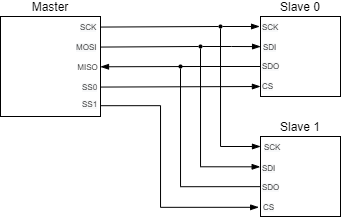
\includegraphics[scale=0.5]{figures/hcis/spi_master_slave.png}
		\caption{Aufbau einer SPI-Bus Verbindung}
	\end{center}
\end{figure}

\newpage

\section{Programmiersprachen}

\subsection{Python}

Python ist eine interpretierte, interaktive, objektorientierte Programmiersprache. Sie enthält Module, Ausnahmen, dynamische Typisierung, dynamische Datentypen auf sehr hoher Ebene und Klassen. Der Code wird automatisch zu Bytecode kompiliert und ausgeführt. Daher eignet sich Python zur Verwendung als Skriptsprache, Implementierungssprache für Webanwendungen. Ebenso kann sie in C und C ++ erweitert werden, wodurch Python die Geschwindigkeit bereitstellen kann, die für rechenintensive Aufgaben erforderlich ist. Aufgrund seiner starken Strukturierungskonstrukte und seiner konsequenten Verwendung von Objekten und objektorientierter Programmierung ermöglicht Python das Schreiben klarer, logischer Anwendungen für kleine und große Aufgaben. Es verfügt über Integrierte Datentypen auf hoher Ebene: Zeichenfolgen, Listen, Wörterbücher, sowie die üblichen Kontrollstrukturen: if, if-else, if-elif-else, while und noch viel mehr. Ebenso gibt es eine sehr große Anzahl an Bibliotheken, welche sonst schwere Aufgaben sehr einfach gestalten.\footnote{vgl- \autocite{python}, Abschnitt 1.1}

\begin{lstlisting}[language=Python, caption={Hello World Programm in Pyhton},captionpos=b]
	
print("Hello World")
	
\end{lstlisting}

\subsection{JavaScript}

JavaScript ist eine benutzerfreundliche Skriptsprache für Objekte, mit der Live-Online-Anwendungen erstellt werden können, die Objekte und Ressourcen auf Clients und Servern miteinander verknüpfen. Während Java von Programmierern zum Erstellen neuer Objekte und Applets verwendet wird, wurde JavaScript für HTML-Seitenautoren und Entwickler von Unternehmensanwendungen entwickelt, um das Verhalten von Objekten, die entweder auf dem Client oder auf dem Server ausgeführt werden, dynamisch zu skripten. JavaScript ist kann von Personen mit wenig oder keiner Programmiererfahrung verwendet werden, um schnell komplexe Anwendungen zu erstellen. Das Design von JavaScript ist speziell für das Internet und die Erstellung netzwerkzentrierter Anwendungen entwickelt worden. \footnote{vgl. \cite{javascript}, Einleitung}

\begin{lstlisting}[language=JavaScript, caption={Hello World Programm in JavaScript},captionpos=b]
	
console.log('Hello World');
	
\end{lstlisting}

\newpage




\chapter{Mechanische Umsetzung}
\fancyfoot[C]{Schmeisser}
\section{Section}

\chapter{Akku und Ladekonzept}
\fancyfoot[C]{Kern}
\section{Section}

%% Übersicht %%%%%%%%%%%%%%%%%%%%%%%%%%%%%%%%%%%%%%%%%%%%%%%
\section{Übersicht}


\subsection{Aufgaben der Energieversorgung}

\subsection{Aufgaben des Batteriemanagement}

\subsection{Allgemeine Übersicht der Elektroinstallation}

%% Batteriemanagement %%%%%%%%%%%%%%%%%%%%%%%%%%%%%%%%%%%%%%%%%
\section{Batteriemanagement}

\subsection{Akkumulatoren}
\subsubsection{Lithiumbatterien}
Die geplanten Funktionen des Antriebssystems lassen sich grob in zwei Grundfunktionen einteilen.

\begin{itemize}
	\item Der Antrieb - Translation ist eine Grundfunktion eines jeden Verkehrsmittels
	\\ Durch die Umwandlung der elektrischen in kinetische Energie erfährt 
	\\ das gesamte System eine Translation.
	\item Die Steuereinheit - Steuerung und Kommunikation mit anderen Betriebsmitteln
	\\ Realisiert durch In- und Outputs, Datenübetragung mithilfe des CAN-Buses 
\end{itemize}

Nun Unterscheiden wir zwischen dem Hardware- und dem Softwareaufbau des Antriebssystems.

\newpage

\chapter{Antriebsstrang}
\fancyfoot[C]{Lackner}


%% Übersicht %%%%%%%%%%%%%%%%%%%%%%%%%%%%%%%%%%%%%%%%%%%%%%%
\section{Übersicht}
Die Hauptaufgabe des Anrtiebssystems ist die Umwandlung der, von dem Akkumulator zur Verfügung gestellten, elektrischen Energie in die kinetische Antriebsenergie. Diese tritt zuerst kreisförmig am Motor auf und wird zunächst über das Direkt-Getriebe umgeformt bzw. auf die passende Drehzahl gebracht, anschließend wird die kreisförmige kinetische Energie mithilfe des Hinterrades auf die Straße übertragen und das ganze Motorrad beschleunigt. Neben dem Antrieb des Motorrades hat die Motorsteuerung noch weitere Bedeutung als Steuereinheit, diese fungiert als Bindemittel zwischen dem Human-Computer Interacting System und den elektrischen Anforderungen an das Gesamtsystem.


\subsection{Grundfunktionen des Systems}
Die geplanten Funktionen des Antriebssystems lassen sich grob in zwei Grundfunktionen einteilen:

\begin{itemize}
	\item Der Antrieb - Translation ist eine Grundfunktion eines jeden Verkehrsmittels
	\\ Durch die Umwandlung der elektrischen Energie in kinetische Energie erfährt 
	\\ das gesamte System eine Beschleunigung in Fahrtrichtung.
	\item Die Steuereinheit - Steuerung und Kommunikation mit anderen Betriebsmitteln
	\\ Realisiert durch In- und Outputs, Datenübetragung mithilfe des CAN-Buses 
\end{itemize}

Um auf die einzelnen Details des Antriebssystems besser eingehen zu können, unterscheiden wir zwischen dem Hardwareaufbau und dem Softwareaufbau des Antriebssystems.

\newpage



%% Hardwareaufbau %%%%%%%%%%%%%%%%%%%%%%%%%%%%%%%%%%%%%%%%%%%%%%%
\section{Hardwareaufbau des Antriebssystems}
Der grundsätzliche Hardwareaufbau des Antriebssystems lässt sich in zwei galvanisch getrennte Stromkreise und der mechanischen Umsetzung unterscheiden:

\begin{itemize}
	\item Mechanische Umsetzung (Kraftübertragung und Montage) 
	\\ Umfasst das Getriebe und die Befestigung aller Komponenten am Rahmen.
	\item Der Laststromkreis
	\\ Beinhaltet die Verbindung des Motorcontrollers mit dem Motor und dem Akkumulator.
	\item Der Steuerstromkreis
	\\ Beinhaltet alle elektrischen Verbindungen, welche mithilfe des 35-poligen
	\\ Niederleistungs-Steckers mit dem Motorcontroller verbunden sind.
\end{itemize}

\newpage



%% Mechanische Umsetzung %%%%%%%%%%%%%%%%%%%%%%%%%%%%%%%%%%%%%%%%%%%%%%% 
\subsection{Mechanische Umsetzung}
Die Fertigung des Getriebes und die Montage der einzelnen Betriebsmittel wurde vollständig von Tobias Schmeisser übernommen.
--> link

\newpage



%% Der Laststromkreis %%%%%%%%%%%%%%%%%%%%%%%%%%%%%%%%%
\subsection{Der Laststromkreis}
Der Laststromkreis befasst sich mit allen leistungsführenden Betriebsmitteln des Antriebssystems. Hierbei unterscheiden wir zwischen zwei Grundfunktionen:

\begin{itemize}
	\item Elektrische Energieübertragung
	\\ Umfasst die elektrische Verbindung von Motor, Motorcontroller und Akkumulator. 						\\ Realisiert durch einfache Leitungen, um Leistungen übertragen zu können.
	\item Schutz aller Komponenten vor möglichen Beschädigungen (Leitungsschutzorgane)
	\\ Beinhaltet eine Schmelzsicherung zum Schutz vor Überströmen und ein 									\\ Hochleistungs-Relais, um im Fehlerfall den kreis öffnen zu können und damit  		
	\\ eine galvanische Trennung des Antriebs und der Energieversorgung gewährleisten zu können.
\end{itemize}

\begin{figure}[H]
	\begin{center}
		%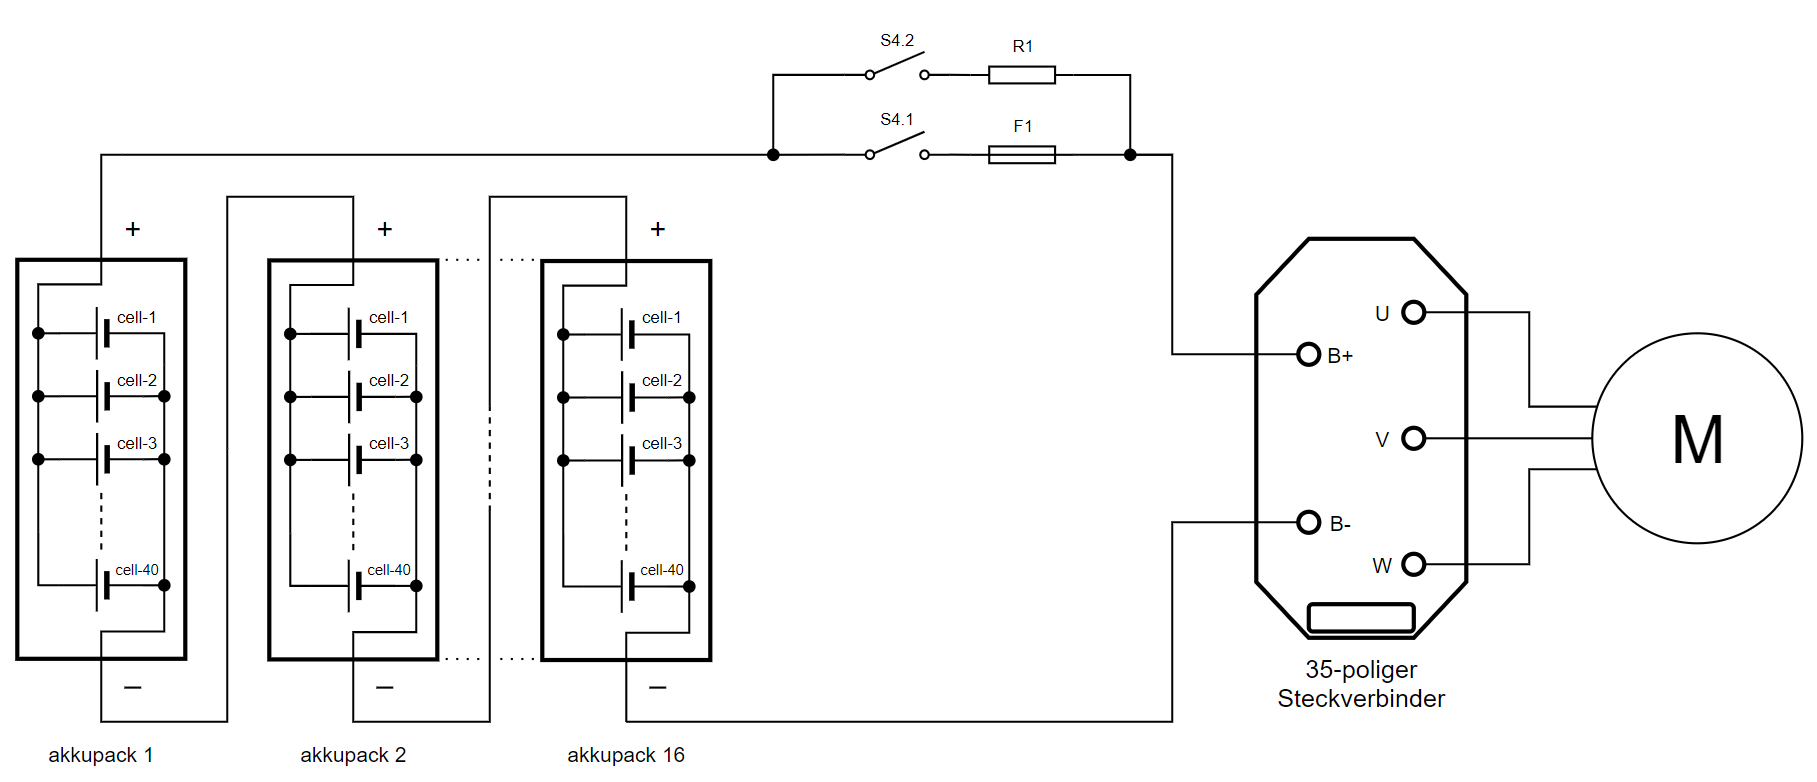
\includegraphics[scale=0.5]{figures/hcis/Antrieb_Laststromkreis.png}
		\caption{Grundaufbau des Laststromkreises}
	\end{center}
\end{figure}

\newpage



%% Elektrische Energieübertragung %%%%%%%%%%%%%%%%%%%%%%%%%%%%%%%%%
\subsubsection{Elektrische Energieübertragung}
Um die benötigte elektrische Energie übertragen zu können, müssen die Leitungen an den Leistungsverbrauch des Verbrauchers (Motor) angepasst werden. Bei einer zu hohen Stromaufnahme (Überlast) des Motors kann es zu einer übermäßigen Erwärmung der Leitungen bis hin zu dauerhaften Beschädigungen, wie durchschmorren der Isolierung oder sogar einen Leitungsbrand, führen. Um dies verhindern zu können, müssen die Leitungen an die Stromaufnahme des Motors angepasst werden. Das heißt, der zulässige Dauerstrom der Leitungen muss den maximalen Dauerstrom des Motors bzw. den maximalen Dauerstrom, welcher durch den Akkumulator zur Verfügung gestellten werden kann, übersteigen.

Berechnung:
In diesem Abschnitt befassen wir uns zunächst mit der Berechnung aller Ströme, die wir zur Auswahl der richtigen Leitungen benötigen. Bei der Auswahl von Leitungen muss man grundsätzlich den Querschnitt und die Länge der Leitung an die benötigte Stromaufnahme des Motors anpassen.

Auswahl:

Fazit:

\newpage



%% Leitungsschutzorgane %%%%%%%%%%%%%%%%%%%%%%%%%%%%%%%%%
\subsubsection{Leitungsschutzorgane}
Die Aufgabe der Leitungsschutzorgane ist es, bei unerwarteten Überströmen oder in einem Fehlerfall den Laststromkreis zu öffnen und damit den Motor bzw. Motorcontroller und den Akkumulator galvanisch zu trennen, um mögliche Beschädigungen an den Komponenten oder an den Leitungen verhindern zu können. Da jedoch ungewünschte Fehlauslösungen zum sofortigen Stillstand des Motorrades führen und eventuell sogar benötigte Wartungen (Wechsel der durchgebrannten Schmelzsicherung) nach sich ziehen, müssen diese Leitungsschutzorgane sehr sorgfältig ausgewählt werden. Eine Überdimensionierung ist ebenso unerwünscht, denn dies hat nicht nur höhere Anschaffungskosten zur folge. Bei Überdimensionierung der Schmelzsicherung, löst diese zu spät aus und hat damit nur mehr eine sehr geringe bis gar keine Schutzfunktion mehr. 

Berechnung:

Auswahl:

Fazit:

\newpage



%% Der Steuerstromkreis %%%%%%%%%%%%%%%%%%%%%%%%%%%%%%%%%%%%%%%%%%%%%%%
\subsection{Der Steuerstromkreis}
\subsubsection{Übersicht Ein- Ausgänge}
Der Steuerstromkreis befasst sich mit allen elektrischen Verbindungen, welche über den  35-poligen Niederleistungs-Stecker mit dem Motorcontroller verbunden sind. Hierbei unterscheiden wir grundsätzlich zwischen drei verchiedenen Ports, welche nochmals unterkategorisiert werden können:

\begin{itemize}
	\item Eingänge (Inputs)
	\\ - Digitale Eingänge (Digital Inputs)
	\\ - Analoge Eingänge (Analog Inputs)
	\\ - Gas- und Bremseingänge (Throttle and Brake Inputs)
	\\ - Positionsrückmeldung vom Encoder (Position-feedback Input)
	\\ - Prozessorversorgung und Spulenrücklauf (KSI and Coil Return)
	\item Ausgänge (Outputs)
	\\ - Analoge Ausgänge (Analog Outputs)
	\\ - Digitale und Pulsweitenmodulierbare Ausgänge (Digital and PWM Outputs)
	\\ - Spannungsversorgungs-Ausgänge (Power Supply Outputs)
	\item Kommunikation (Communication)
	\\ -  CAN-Bus (CAN-Port)
	\\ -  Serielle Schnittstelle (Serial-Port)
\end{itemize}

Der Motorcontroller verfügt über viele Pins, welche über mehrere Funktionen verfügen, es muss jedoch eine dieser Funktionen ausgewählt werden. Pin 6 zum Beispiel wird eigentlich als digitaler und phasenmodulierbare Ausgang verwendet, bei richtiger Konfiguration kann dieser jedoch auch als digitaler Input verwendet werden. Weiteres kann frei konfiguriert werden, ob man mit diesem Ausgang zum Beispiel das Hochleistungs-Relais oder einen Spannungswandler ansteuern möchte. Um den passenden Pin für eine Anwendung auswählen zu können, muss man jedoch die elektrischen Eigenschaften der Pins genauer unter die Lupe nehmen. Oftmals haben auch die Pins der selben Unterkategorie verschiedene Funktionen, Eingangsimpedanzen oder Toleranzen. 

\begin{figure}[H]
	\begin{center}
		%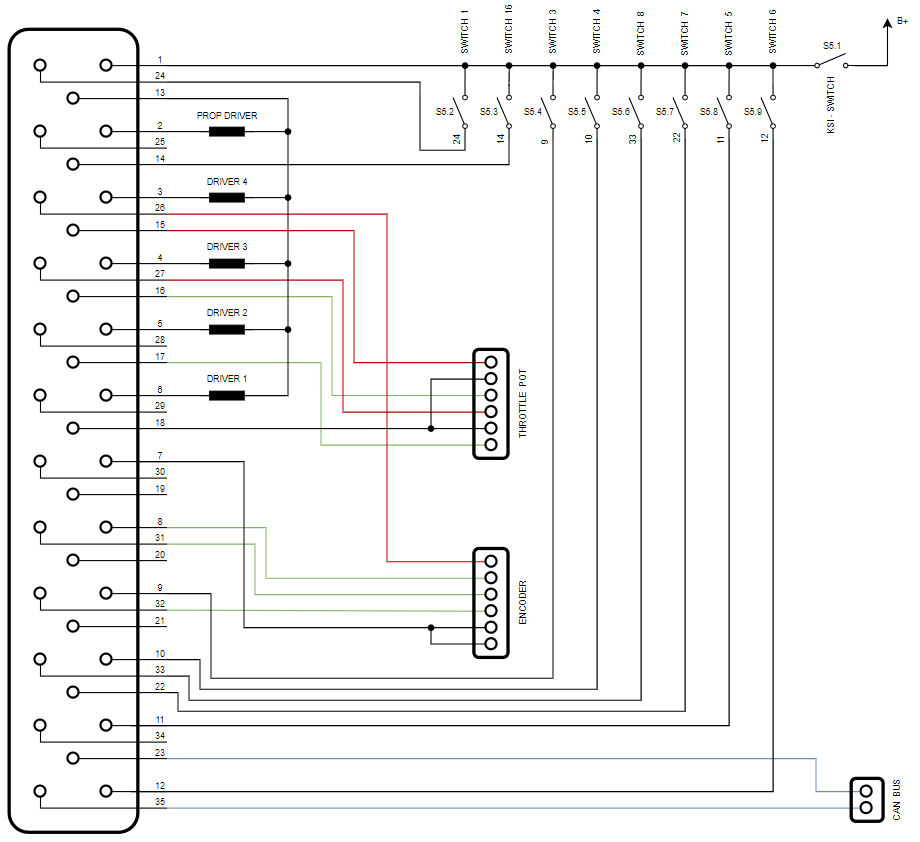
\includegraphics[scale=0.5]{figures/hcis/Antrieb_Steuerstromkreis.png}
		\caption{Grundaufbau des Steuerstromkreises}
	\end{center}
\end{figure}

\newpage



%% Digitale Eingänge (Digital Inputs) %%%%%%%%%%%%%%%%%%%%%%%%%%%%%%%%%%%%%%%%%%%%%%%
\subsubsection{Digitale Eingänge (Digital Inputs)}
Digitale Eingänge (Digital Inputs)
Es gibt insgesamt 16 Pins, die als digitale Eingänge genutzt werden können, jedoch werden sieben Pins davon eigentlich als Ausgänge konfiguriert. 

\begin{figure}[H]
	\begin{center}
		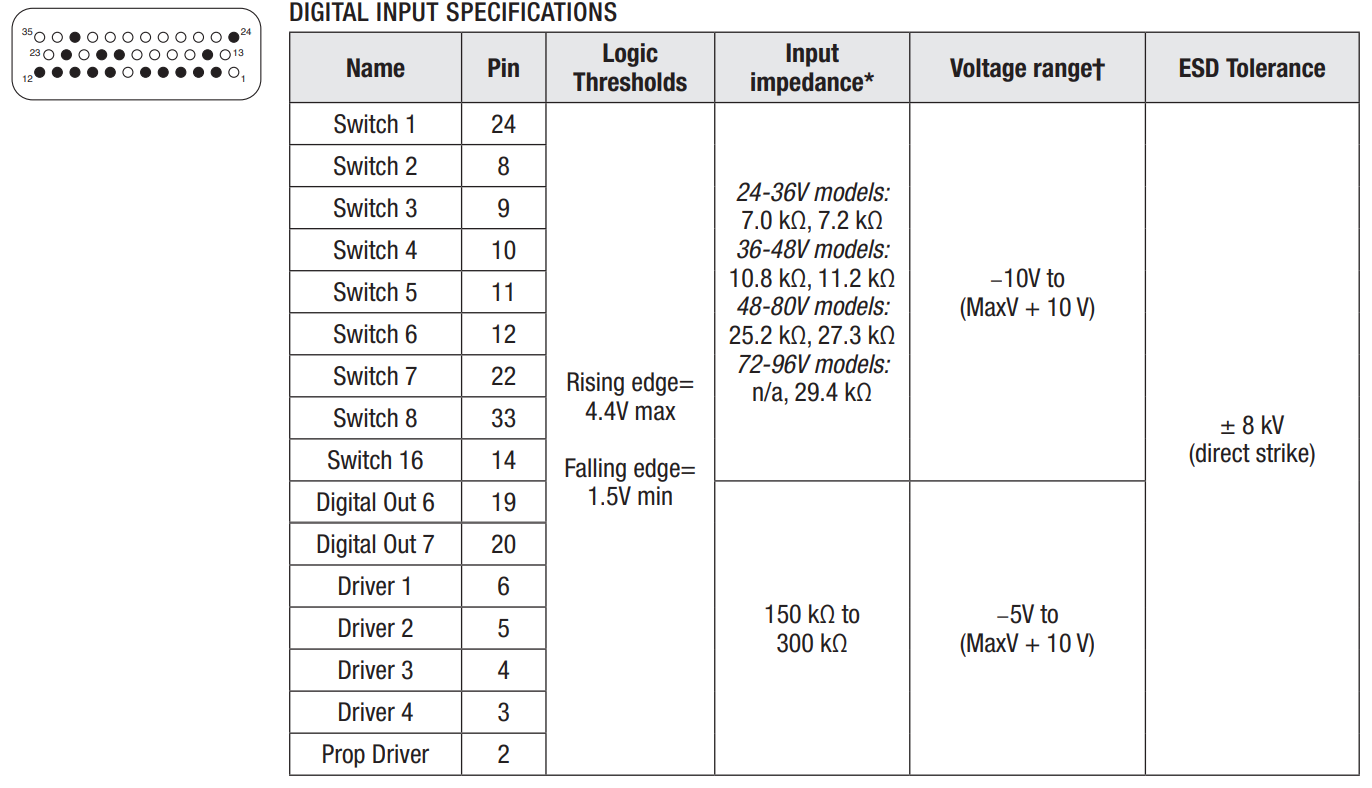
\includegraphics[scale=0.4]{figures/hcis/Digital_Input_Specifications.png}
		\caption{Digital Input Specifications}
	\end{center}
\end{figure}




%% Analoge Eingänge (Analog Inputs) %%%%%%%%%%%%%%%%%%%%%%%%%%%%%%%%%%%%%%%%%%%%%%%
\subsubsection{Analoge Eingänge (Analog Inputs)}
Es gibt insgesamt zwei Pins die als analoge Eingänge verwendet werden können. Ein Pin davon wird jedoch im Normalfall für den Motortemperatur-Sensor verwendet. Die Eingänge, die für das Gas- und Bremspotentiometer verwendet werden, sind in dieser Kategorie nicht aufgelistet, obwohl diese ebenfalls als analoge Eingänge genutzt werden. Diese Pins sind jedoch speziell für die Gas- und Bremssteuerung konfiguriert und sollten im Normalfall auch dafür hergenommen werden.

\begin{figure}[H]
	\begin{center}
		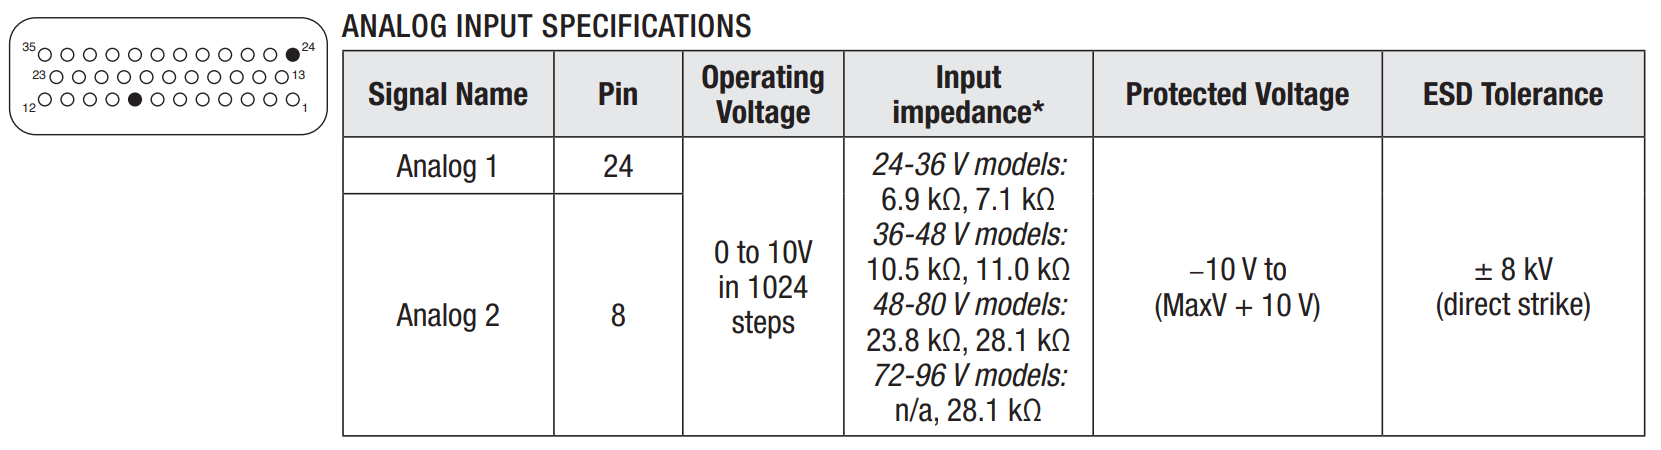
\includegraphics[scale=0.4]{figures/hcis/Analog_Input_Specifications.png}
		\caption{Analog Input Specifications}
	\end{center}
\end{figure}



%% Gas- und Bremseingänge (Throttle and Brake Inputs) %%%%%%%%%%%%%%%%%%%%%%%%%%%%%%%%%%%%%%%%%%%%%%%
\subsubsection{Gas- und Bremseingänge (Throttle and Brake Inputs)}
Die zwei Gas- oder Bremssteuerungs-Eingänge können unabhängig von einander programmiert werden. Sie sind optimiert für die Anwendung mittels Spannungssteuerung, 2-Draht Widerstandssteuerung oder 3-Draht Widerstandssteuerung. Bei der Spannungssteuerung benötigt man die Pins Pot Wiper und I/O Ground, bei der 2-Draht Widerstandssteuerung Pot Wiper und Pot Low und bei der 3-Draht Widerstandssteuerung Pot High, Pot Wiper und Pot Low. In unserem Fall benutzen wir beide Steuerungs-Eingänge für die 3-Draht Widerstandssteuerung, da der Gasdrehgriff über eine Drahtbrucherkennung (zwei unabhängige 3-Draht Potentiometer-Ausgänge) verfügt.

\begin{figure}[H]
	\begin{center}
		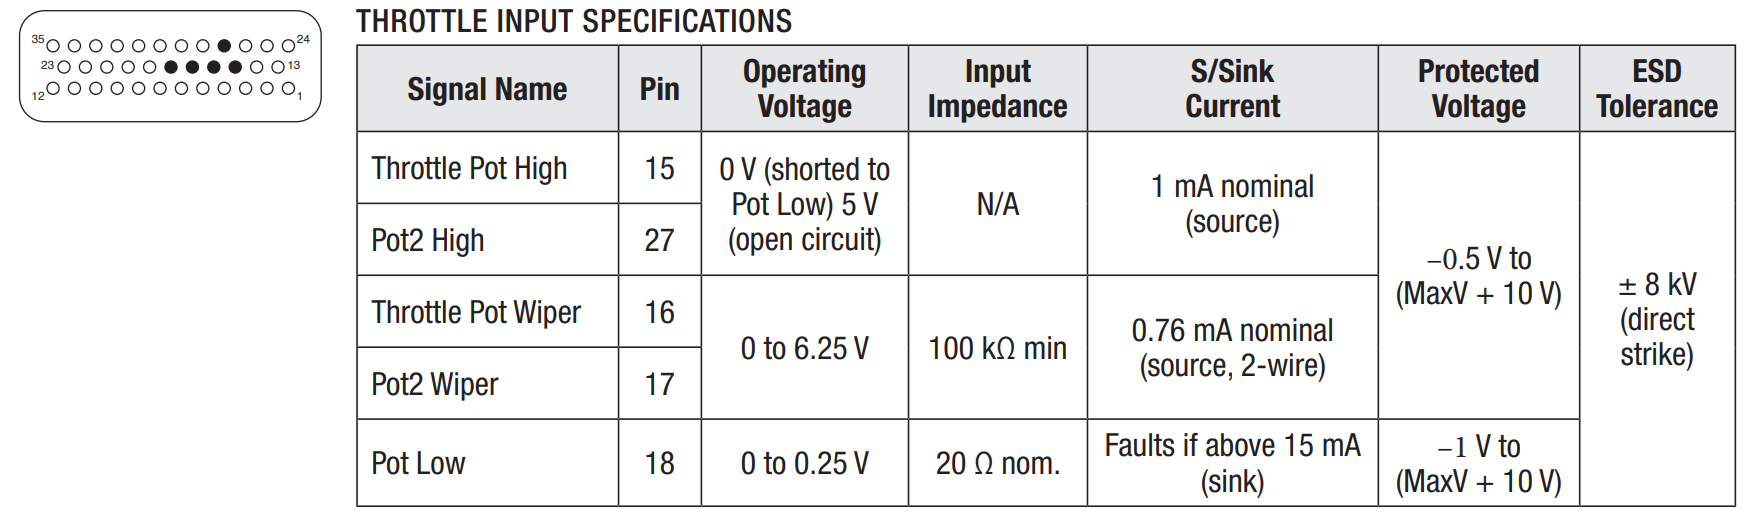
\includegraphics[scale=0.5]{figures/hcis/Throttle_Input_Specifications.png}
		\caption{Throttle Input Specifications}
	\end{center}
\end{figure}



%% Positionsrückmeldung vom Encoder (Position-feedback Input) %%%%%%%%%%%%%%%%%%%%%%%%%%%%%%%%%%%%%%%%%%
\subsubsection{Positionsrückmeldung vom Encoder (Position-feedback Input)}
Diese zwei Pins sind intern dafür konfiguriert, die aktuelle Position der Motorwelle einzulesen, um eine optimale feldorienterte Ansteuerung des Motors durchführen zu können. Dabei gibt es die Möglichkeiten über einen Quadratur-Encoder oder einen Sin/Cos-Encoder. Da in dem Ashwoods-Motor ein Sin/Cos-Sensor verbaut ist, wurde dies vorab bei dem Motorcontroller eingestellt.

\begin{figure}[H]
	\begin{center}
		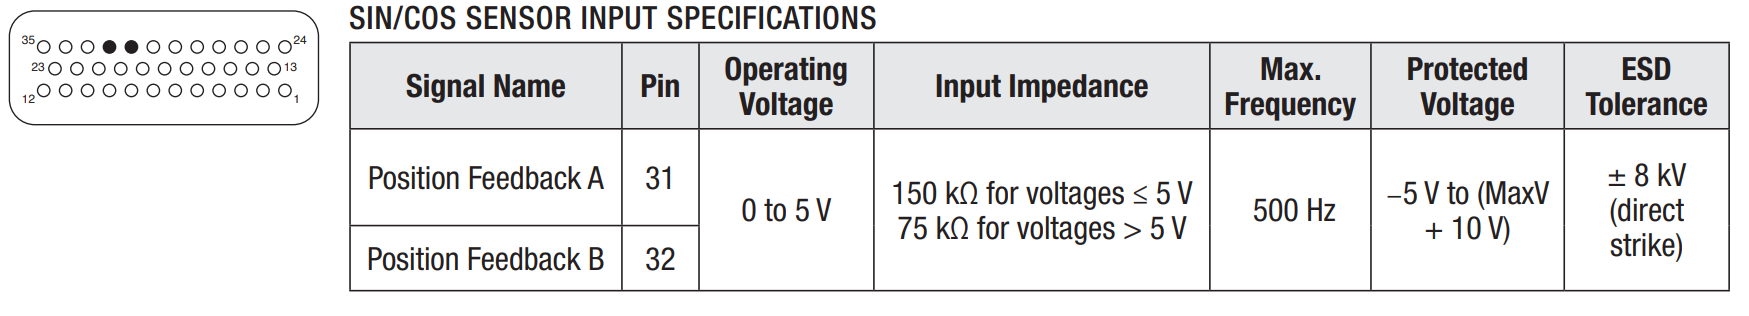
\includegraphics[scale=0.5]{figures/hcis/SinCosSensor_Input_Specifications.png}
		\caption{Sin/Cos Sensor Input Specifications}
	\end{center}
\end{figure}



%% Prozessorversorgung und Spulenrücklauf (KSI and Coil Return) %%%%%%%%%%%%%%%%%%%%%%%%%%%%%%%%%%%%%%%%
\subsubsection{Prozessorversorgung und Spulenrücklauf (KSI and Coil Return)}
Der KSI-Eingang stellt die elektrische Versorgung aller Niederleistungs-Schaltkreise zur Verfügung. Dies  beinhaltet ebenfalls die Versorgung aller Ausgänge und die Kondensator-Vorlade-Funktion, welche dazu dient, die Kondensatoren vorzuladen, um hohe Einschaltströme zu verhindern. Der Spulenrücklauf ist speziell für den Rücklauf der Pulsweitenmodulierbare-Ausgänge konfiguriert worden, um ein übrmäßiges Schaltrauschen zu verhindern.

\begin{figure}[H]
	\begin{center}
		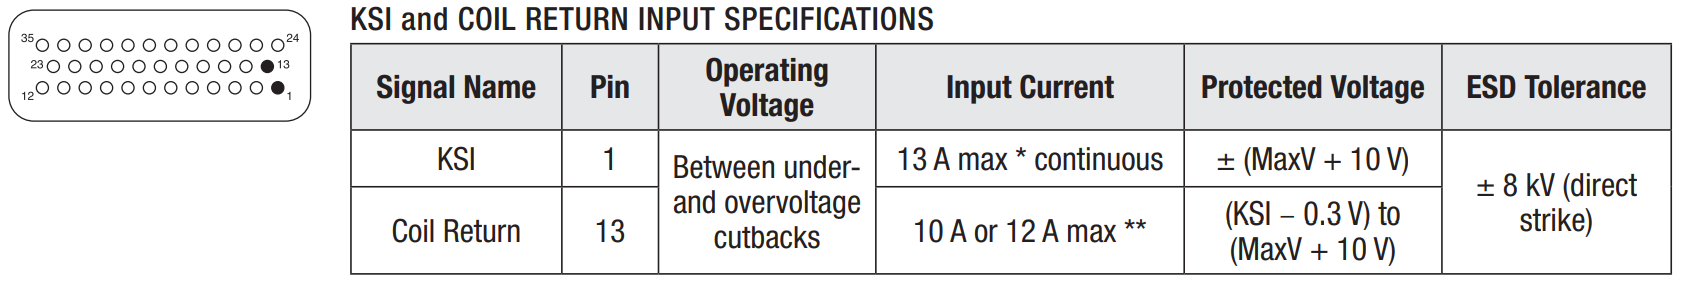
\includegraphics[scale=0.5]{figures/hcis/KSI_CoilReturn_Input_Specifications.png}
		\caption{KSI and Coil Return Input Specifications}
	\end{center}
\end{figure}



%% Analoge Ausgänge (Analog Outputs %%%%%%%%%%%%%%%%%%%%%%%%%%%%%%%%%%%%%%%%%%%%%%%
\subsubsection{Analoge Ausgänge (Analog Outputs)}
Der analoge Ausgang kann ein Spannungssignal von 0 bis 10V ausgeben. Dieser Ausgang ist für die Ausgabe über Anzeigeinstrumente, wie zum Beispiel eine Anzeige über den aktuellen Ladestand des Akkumulators, vorgesehen.

\begin{figure}[H]
	\begin{center}
		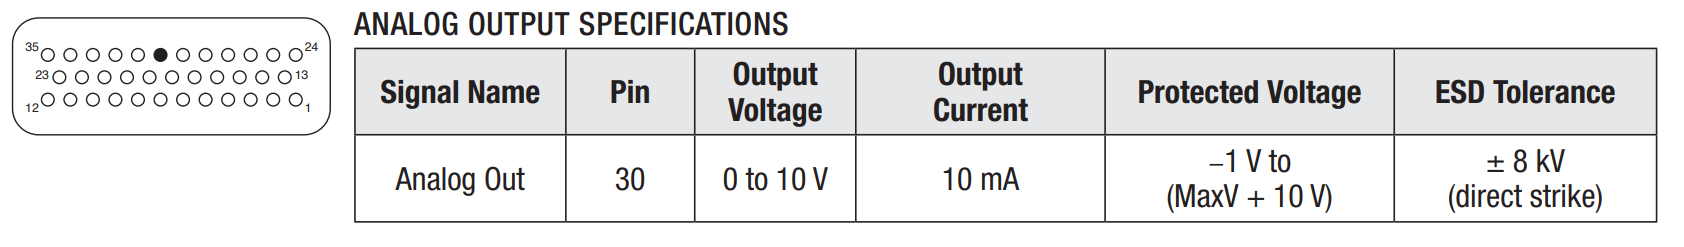
\includegraphics[scale=0.5]{figures/hcis/Analog_Output_Specifications.png}
		\caption{Analog Output Specifications}
	\end{center}
\end{figure}



%% Digitale und Pulsweitenmodulierbare Ausgänge (Digital and PWM Outputs) %%%%%%%%%%%%%%%%%%%%%%%%%%%%%%
\subsubsection{Digitale und Pulsweitenmodulierbare Ausgänge (Digital and PWM Outputs)}
Es gibt insgesamt 7 digitale Ausgänge, wovon jedoch nur 5 für eine Pulsweitenmodulation konfiguriert werden können. Diese Ausgänge sind für induktive Lasten, wie zum Beispiel den Hauptschütz oder eine elektromagnetische Bremse, vorgesehen. Rein ohmsche Lasten können ebenfalls gesteuert werden, jedoch darf der zulässige Spitzenstrom nicht überschritten werden. Der Proportional Driver kann bei richtiger Konfiguration ebenfalls für die Anzeige eines Tachometers hergenommen werden. Diese Gruppe kann ebenfalls als digitaler Eingang benutzt werden.

\begin{figure}[H]
	\begin{center}
		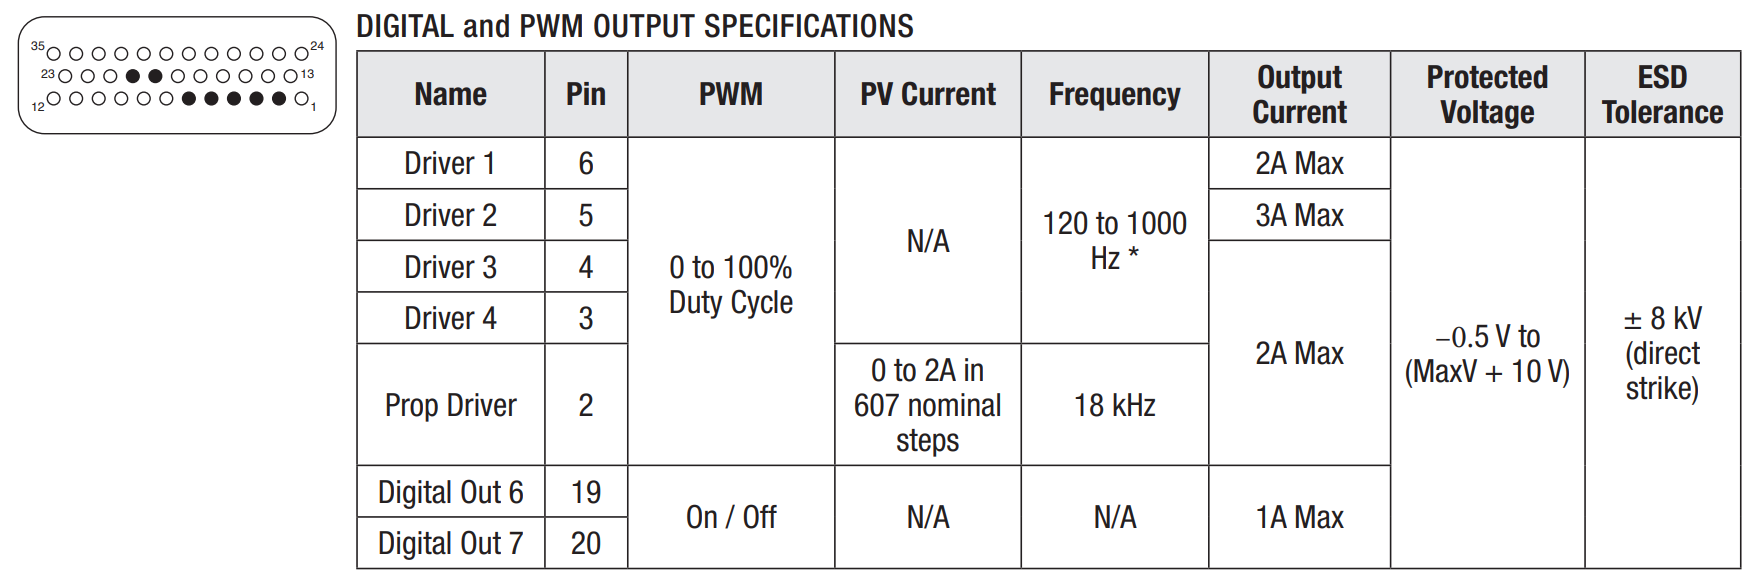
\includegraphics[scale=0.5]{figures/hcis/Digital_PWM_Output_Specifications.png}
		\caption{Digital and PWM Output Specifications}
	\end{center}
\end{figure}



%% Spannungsversorgungs-Ausgänge (Power Supply Outputs) %%%%%%%%%%%%%%%%%%%%%%%%%%%%%%%%%%%%%%%%%%%%%%%
\subsubsection{Spannungsversorgungs-Ausgänge (Power Supply Outputs)}
Um kleine Schaltkreise, wie zum Beispiel einen LED-Indikator oder die Positionsrückmeldung vom Encoder, mit Spannung versorgen zu können, gibt es zwei dafür vorgesehene Spannungsversorgungs-Ausgänge mit einem Pin für 5V und 12V. Für diese Anwendungen gibt es ebenfalls noch einen Rücklauf, der als I/O Ground definiert wurde.

\begin{figure}[H]
	\begin{center}
		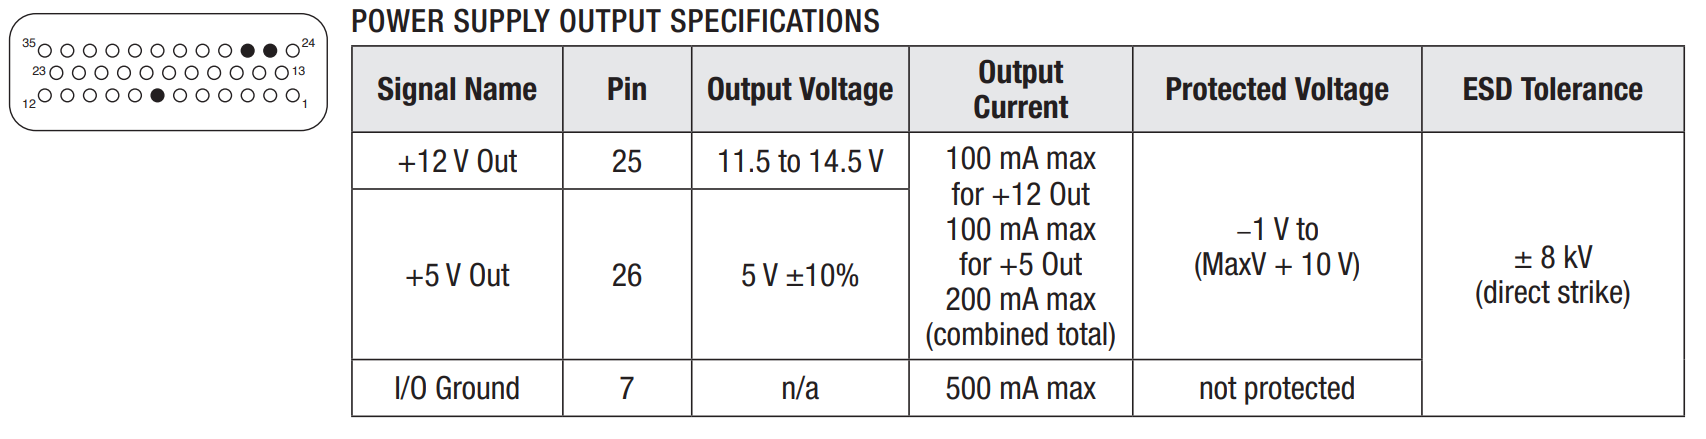
\includegraphics[scale=0.5]{figures/hcis/Power_Supply_Output_Specifications.png}
		\caption{Power Supply Output Specifications}
	\end{center}
\end{figure}


%% Kommunikations-Ports %%%%%%%%%%%%%%%%%%%%%%%%%%%%%%%%%%%%%%%%%%%%%%%
\subsubsection{Kommunikations-Ports}
Für die Kommunikation mit anderen Betriebsmitteln stellt uns der Motorcontroller zwei Möglichkeiten zur Verfügung, den CAN-Bus und die seielle Schnittstelle. Da sich unser Projektteam auf die Nutzung des CAN-Buses geeinigt hat, wird die serielle Schnittstelle nicht verwendet. Die zwei Pins CAN Term High und CAN Term Low werden ebenfalls nicht benötigt, denn diese dienen nur dazu, den CAN-Bus vorübergehend funktionsunfähig zu schalten. Programmtechnisch gibt es drei Möglichkeiten vom Motorcontroller zur Konfiguration des CAN-Buses, dies wird jedoch im Punkt Software genauer erklärt.

\begin{figure}[H]
	\begin{center}
		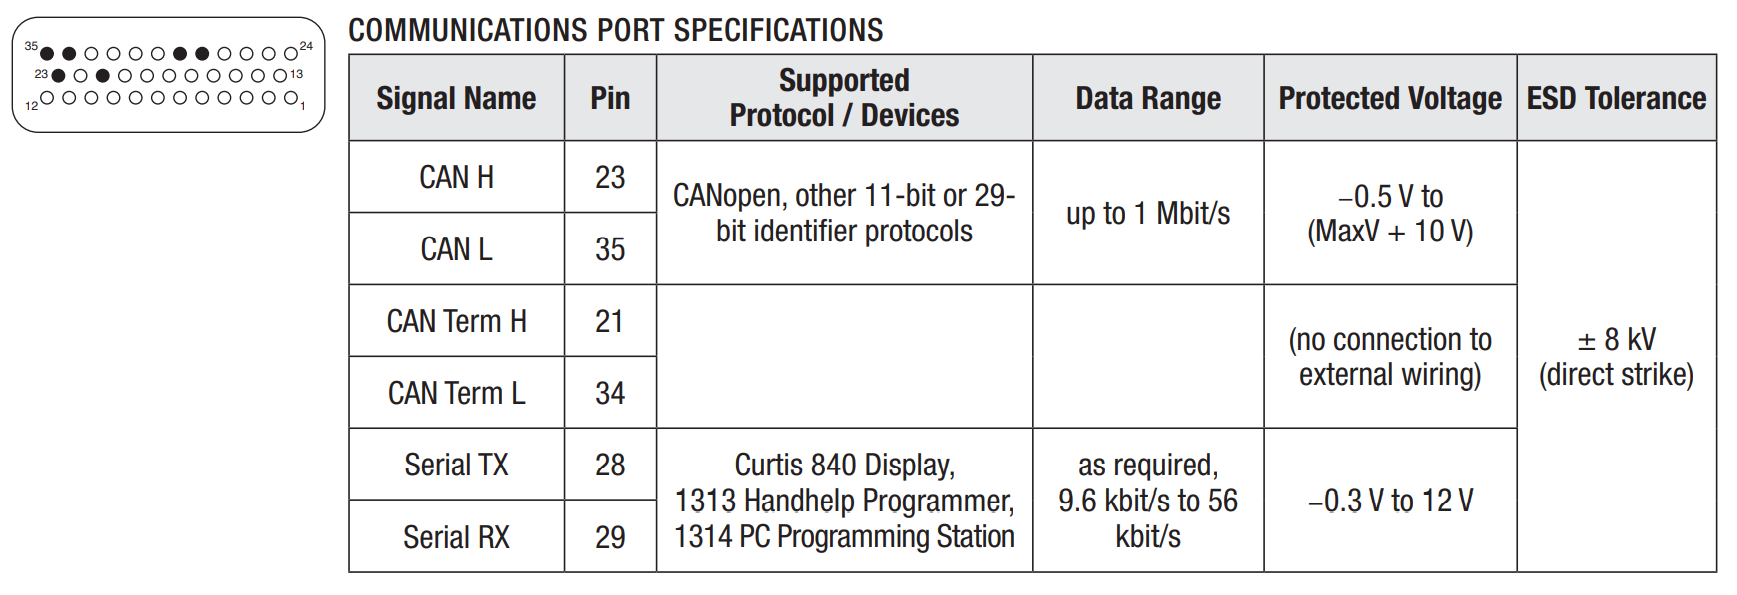
\includegraphics[scale=0.5]{figures/hcis/Communications_Port_Specifications.png}
		\caption{Communications Port Specifications}
	\end{center}
\end{figure}



\newpage



%% Softwareaufbau %%%%%%%%%%%%%%%%%%%%%%%%%%%%%%%%%%%%%%%
\section{Softwareaufbau des Antriebssystems}


%% Steuerung der In- und Outputs %%%%%%%%%%%%%%%%%%%%%%%%%%%%%%%%%%%%%%%%%%%%
\section{ Steuerung der Ein- und Ausgänge (I/O Assingment)}
\subsection{Funktionen}
\subsection{Zuweisung}


%% Drehmomentsteuerung %%%%%%%%%%%%%%%%%%%%%%%%%%%%%%%%%%%%%%%%%%%%
\section{Drehmomentsteuerung (Torquecontrol)}
\subsection{Grundfunktion}
\subsection{Parameter}


%% Kommunikation %%%%%%%%%%%%%%%%%%%%%%%%%%%%%%%%%%%%%%%%
\section{Kommunikation (CAN-Bus)}
\subsection{Grundfunktion}
\subsubsection{Parameter}


\fancyfoot[C]{Kronberger}

%% Human-Computer Interaction System %%%%%%%%%%%%%%%%%%%%%%%

\chapter{Human-Computer Interaction System}

\section{Übersicht}

Das Human-Computer Interaction System ist, wie der Name schon sagt, die Komponente, welche als Schnittstelle zwischen dem Nutzer und dem gesamten elektrischen System dient. Durch es sollte die fehlerfreie Nutzung der Funktionen des Motorrades gewährleistet sein. Ebenso sollte es wichtige Fahrdaten und andere Informationen speichern und dem User anzeigen können.\\
Wichtig ist das System, trotz der großen Komplexität, so intuitiv und nutzerfreundlich wie möglich zu gestalten.

\subsection{Grundfunktionen des Systems}

Die geplanten Funktionen des HCIS \footnote{Abkurzümg: Human-Computer Interaction System} lassen sich grob in vier Grundfunktionen einteilen.

\begin{itemize}

	\item \textbf{Steuerung der Peripherie} \medskip\\
	Die Schalter und Buttons am Lenker, welche zuvor über den Kabelbaum die Leuchten, Blinker und die Hupe gesteuert haben, werden nun über die General-purpose input/output (GPIO) des Raspberry Pi Mikrocomputers gesteuert.

	\item \textbf{Graphische Benutzeroberfläche}\medskip\\
Dient der Anzeige wichtiger Fahr- und Ladedaten, welche entweder in Echtzeit oder über die Datenbankschnittstelle abgerufen und graphisch angezeigt werden können.

	\item \textbf{Kommunikation mit den Steuereinheiten des Motorrades} \medskip\\
	Über CAN-Bus werden Daten von dem Batterie Management Systems (BMS) und der Curtis Motorsteuerung empfangen und an die Benutzeroberfläche zur Anzeige und an die Datenbankschnittstelle zur Langzeitsicherung der Fahrdaten weiter gegeben.

	\item \textbf{Speichern der relevanten Fahrdaten über die Datenbankschnittstelle} \medskip\\
Die über den CAN-Bus empfangenen Daten werden sofort an die Datenbankschnittstelle (Handler) weitergegeben um die Daten für Datenauswertung und Testberichte zu speichern. Ebenso bezieht das Diagnosesystem der Benutzeroberfläche die Daten über diese Schnittstelle.

\end{itemize}

\newpage

\subsection{Steuereinheit}

Als Basis zur Auswahl der Steuereinheit wurden die zuvor erläuterten Grundfunktionen herangezogen genommen. Die Ausgewählte Steuereinheit sollte diese erfüllen können und ebenso Potential zur Erweiterung der Funktionen bieten. Genauso wichtig war das eine große Flexibilität und Individualität erreicht werden kann, um nicht in der Umsetzung unserer Ideen eingeschränkt zu sein. Zur Auswahl standen verschiedene Speicherprogrammierbare Steuerungen und Mikrocomputer, doch letzten Endes überzeugte der Mikrocomputer Raspberry Pi.

\begin{figure}[H]
	\begin{center}
		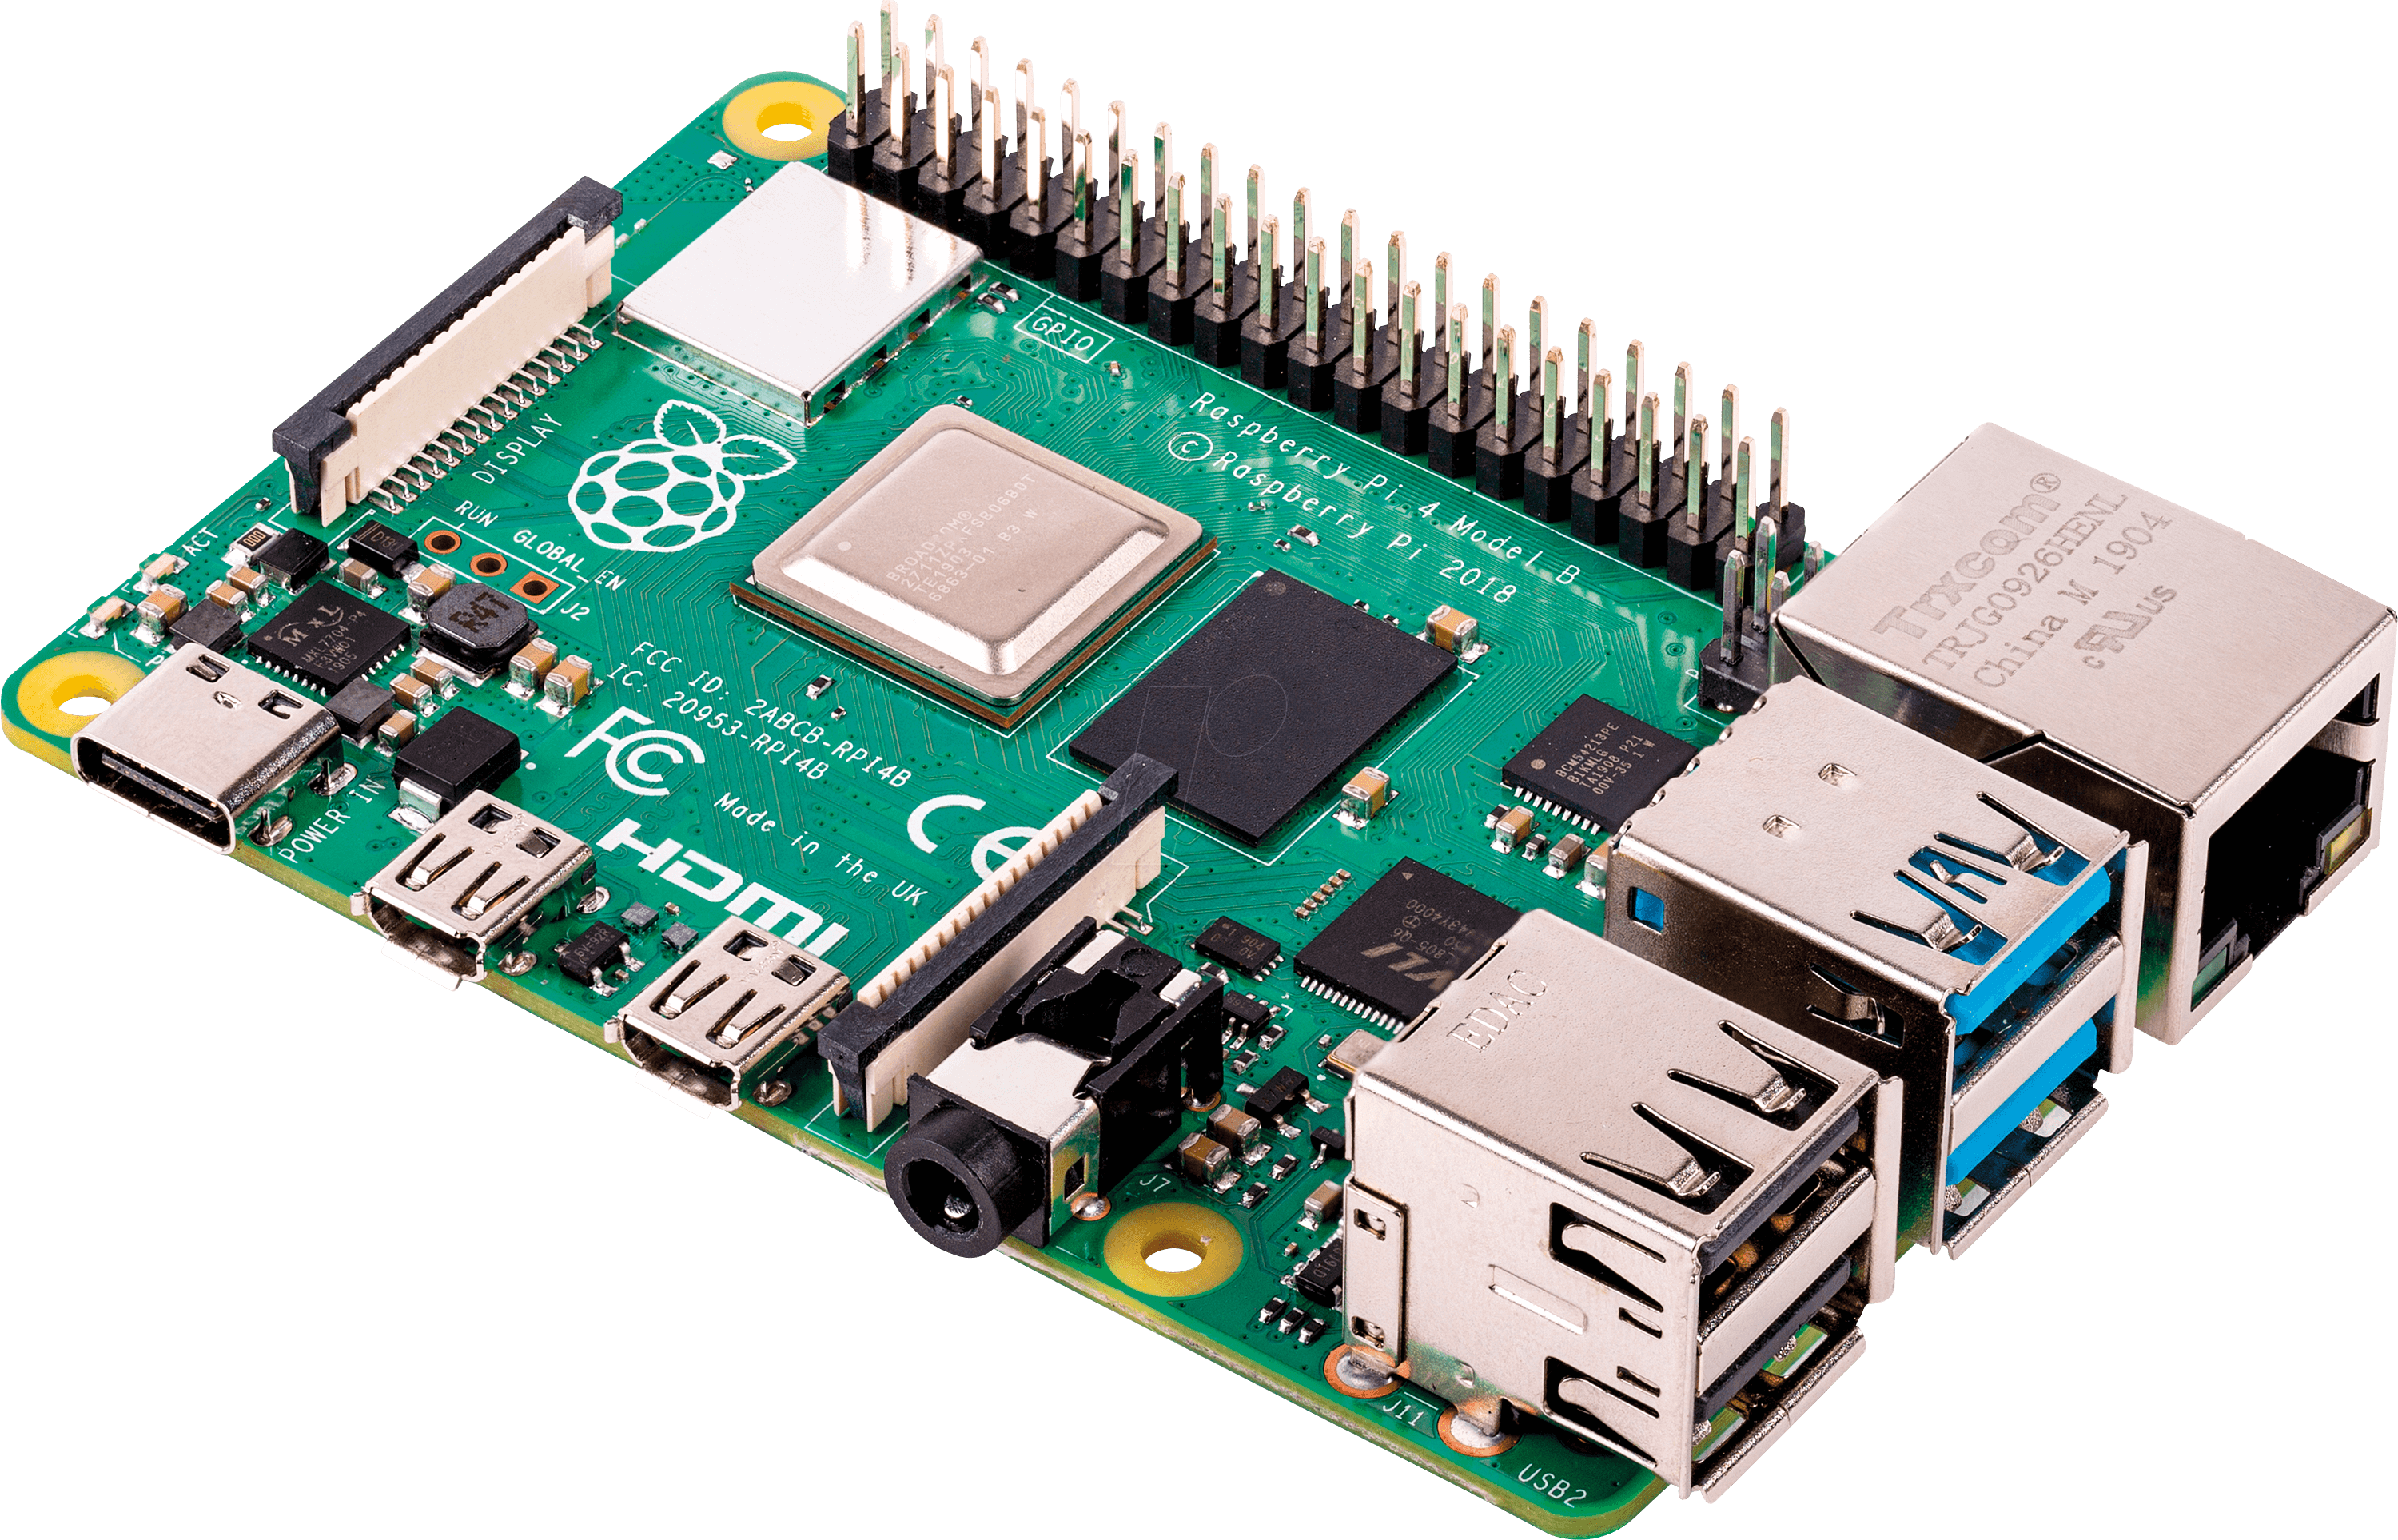
\includegraphics[scale=0.08]{figures/hcis/raspberryPi.png}
		\caption{Raspberry Pi - Steuereinheit des HCIS}
	\end{center}
\end{figure}

\subsection{Grundaufbau des Systems}

In der Abbildung \ref{fig:aufbauHCIS} wird der Grundaufbau des Systems und die Datenverbindungen der folgenden  Komponenten veranschaulicht.

\begin{itemize}
	
	\item Raspberry Pi - Die Steuereinheit des Systems.
	\\ Kommuniziert über CAN-Bus mit den anderen Steuerkomponenten des Motorrades.
	
	\item User Input - Die vorhandenen Schalter am Lenker des Motorrads werden direkt mit den Eingängen des Raspberry Pis verbunden. 
	
	\item Peripherie - Die Grundkomponenten des Motorrades wie Scheinwerfer oder Hupe. Diese werden über Relais, welche an die Ausgänge des Raspberry Pis angeschlossen sind, gesteuert.
	
	\item Dashboard - Der Bildschirm zur Anzeige der verarbeiteten Informationen. Dieser wird über HDMI und USB mit dem Raspberry Pi verbunden.
	
\end{itemize}

\begin{figure}[H]
	\begin{center}
		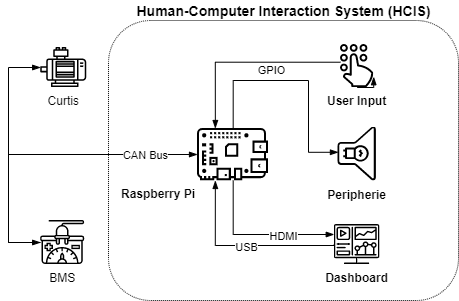
\includegraphics[scale=0.5]{figures/hcis/HCIS_Grundfunktion.png}
		\caption{Grundaufbau des Human-Computer Interaction Systems}
		\label{fig:aufbauHCIS}
	\end{center}
\end{figure}

Nicht in der Abbildung dargestellt ist die Versorgung der einzelnen Komponenten, welche in dem folgenden Abschnitt noch genauer erläutert wird.

\newpage


%% Versorgung %%%%%%%%%%%%%%%%%%%%%%%%%%%%%%%%%%%%%%%%%%%%%%% 

\section{Spannungsversorgung}

\subsection{Aufbau des Versorgungssystems} \label{sec:aufbauversorgung}

Das Versorgungssystem des Motorrades besteht aus zwei Spannungsebenen: Einer 12V Ebene zur Versorgung der Peripherie des Motorrades und einer 5V Ebene, welche nur den Raspberry Pi und seine Komponenten beinhaltet. Diese Ebenen werden durch DC-DC Wandler erzeugt, welche direkt an den Akku des Motorrades angeschlossen werden. \\

Wichtig hierbei ist, dass alle ausgewählten Spannungswandler über einen Kurzschluss- und Überstrom-Schutz verfügen. Dies macht es uns möglich diese Versorgungssysteme, solange die Drähte auch nach dem maximalen Strom der Spannungswandler dimensioniert wurden, ohne jegliche Leitungs- und Überstrom-Schutzorgane aufzubauen. Die Spannungswandler schalten bei jeglichen Fehlern ab und verbrennen die überschüssige Leistung über einen eingebauten Widerstand. Sobald der Fehler behoben wurde, schalten sich die Spannungswandler automatisch wieder ein.

\subsubsection{12V Versorgungsysstem}

Um den Spannungswandler dimensionieren zu können mussten vorher alle Bauteile, welche über die 12V versorgt werden sollten, zusammengefasst werden, um die mindestens benötigte Leistung des Spannungswandlers zu errechnen. 

\begin{table}[H]
	\begin{center}
		\begin{tabular}{|l|c|c|}
			\hline
			\textbf{Bauteilbezeichnung}     & \textbf{Spannung} & \textbf{Leistung} \\ \hline
			Tagfahrlicht           & 12V      & 10W      \\ \hline
			Abblendlicht           & 12V      & 10W      \\ \hline
			Aufblendlicht          & 12V      & 20W      \\ \hline
			Hupe                   & 12V      & 10W      \\ \hline
			Rücklicht              & 12V      & 21W      \\ \hline
			Kennzeichenbeleuchtung & 12V      & 5W       \\ \hline
			Blinker links          & 12V      & 2 x 10W  \\ \hline
			Blinker rechts         & 12V      & 2 x 10W  \\ \hline
			Bildschirm             & 12V      & 12W      \\ \hline
			\textbf{Gesamt}                 & \textbf{12V}      & \textbf{128W}     \\ \hline
		\end{tabular}
			\caption{Berechnung der Leistung des 12V-Systems}
			\label{tab:leistung12V}
	\end{center}
\end{table}

Der Spannungswandler wurde nun nach der größt möglichen Leistung, welche auftritt wenn alle Bauteile gleichzeitig auf Höchstleistung betrieben werden, ausgelegt. Diese maximale Leistung beträgt, wie in der Tabelle \ref{tab:leistung12V} zu sehen, 128 Watt. Um noch Ausbaumöglichkeiten zu gewährleisten und uns nicht dem Leistungslimit des Wandlers zu nähern, haben wir uns für einen 48V-12V, 300 Watt DC-DC Wandler von Mean Well \footnote{Datenblatt: siehe Anhang \ref{app:mw12}} entschieden. 

\subsubsection{5V Versorgungssystem}

Die Leistung des Raspberry Pis ist mit einem Maximum von 6.2 Watt sehr klein und daher ist die Wahl des Spannungswandlers in diesem Fall nicht wirklich davon abhängig. Auch die Komponenten, welche angeschlossen werden, haben grundsätzlich keine erwähnenswerte Wirkleistung und müssen daher nicht genau ein berechnet werden. Nun entschied nur mehr das Preis-Leistungs-Verhältnis sowie die Ausfallsicherheit des Spannungswandlers die Wahl. Daher haben wir uns für einen 48V-5V, 30 Watt DC-DC Wandler von Meanwell \footnote{Datenblatt: siehe Anhang \ref{app:mw5}} entschieden.

\subsubsection{Abschalten der Spannungswandler}

Das Abschalten der Spannungswandler ist nicht notwendig, da diese - wie schon in Abschnitt \ref{sec:aufbauversorgung} erklärt - bei einem anliegenden Fehler automatisch abschalten.
Ebenso wird beim Abschalten des Motorrades über die BMS jegliches andere Bauteil von der Spannungsversorgung getrennt. Was die Spannungswandler vom Entladen des Akkus abhält.  

\newpage

%% Steuerung der Peripherie %%%%%%%%%%%%%%%%%%%%%%%%%%%%%%%%%

\section{Steuerung der Peripherie}

Die Grundfunktionen wie Beleuchtung, Hupe und Blinker werden hier als Peripherie bezeichnet. Diese sollten so einfach wie möglich und vom Lenker aus zu bedienen sein. Ebenso müssen sie verlässlich gesteuert werden können. Daher haben wir uns entschieden diese Funktionen ebenso über den Raspberry Pi zu steuern, da dieser bei einem Fehler der Motorsteuerung über den eingebauten Puffer gespeist werden kann und daher diese wichtigen Funktionen bis zu einem sicheren Stillstand weiter betrieben und gesteuert werden können.\\


Dennoch ist in der Plan in Zukunft die Motorsteuerung, welche ebenso in der Lage wäre die Ausgänge abhängig von den Eingängen zu schalten, diese Aufgabe übernehmen zu lassen, solange die Ausfallsicherheit ebenso gegeben wäre. Der Vorteil dieser Methode ist die Schaffung einer Zentralen Steuereinheit, welche alle Steueraufgaben in einem Bauteil vereinen kann.

\subsection{Hardware}

\subsubsection{Input}

Man kann einen GPIO Pin entweder als Eingang oder als Ausgang betreiben. Als Eingang kann er die Zustände High und Low einnehmen. Zum Beispiel von einem Schalter oder Taster. In der Regel beschaltet man die GPIOs des Raspberry Pis mit Widerständen, um Eingänge auf einen definierten Pegel zu setzten oder um den Strom zu begrenzen. Standardmäßig werden 10k Widerstände benutzt. Ob Pullup oder Pulldown ist grundsätzlich gleichgültig. Wir benutzen für das Einlesen der Eingänge 10k Pulldown Widerstände, um nicht immer eine Spannung an den Eingängen des Raspberry Pis anliegen zu haben.

\begin{figure}[H]
	\begin{center}
		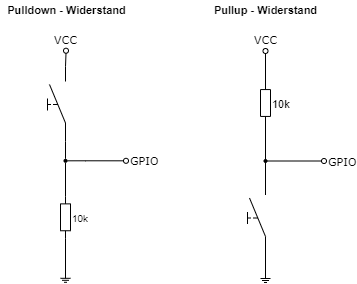
\includegraphics[scale=0.8]{figures/hcis/input.png}
			\caption{Anschlussplan Eingänge}
			\label{fig:input}
	\end{center}
\end{figure}

\textbf{Pullup Widerstand}\\

Bei dem Nutzen eines Pullup Widerstands wird der GPIO Pin mit einem Widerstand auf die Spannnung von VCC gezogen. Der Grundzustand des Eingangs ist dann High. Mit einem Schalter oder Taster wird der Eingang dann gegen Ground gezogen. Das heißt er hat solange der Schalter geschlossen ist, liegt das Massepotential am Eingang an.\\\medskip

\textbf{Pulldown Widerstand}\\

Bei dem Nutzen eines Pulldown Widerstands wird der GPIO Pin mit einem Widerstand auf die Spannnung von Ground gezogen. Der Grundzustand des Eingangs ist dann Low. Mit einem Schalter oder Taster wird der Eingang dann gegen VCC gezogen. Das heißt er hat solange der Schalter geschlossen ist, liegt das Versorgunspotential am Eingang an.

\subsubsection{Output}

Hierbei werden die GPIOs als Ausgang verwendet. Sie sind verbunden mit den Eingängen eines 4 Channel Relais Moduls, welches über die 5V direkt von dem Raspberry Pi gespeist wird. Hiermit ist es nun Möglich die 12V der Perpherie zu schalten und 

\begin{figure}[H]
	\begin{center}
		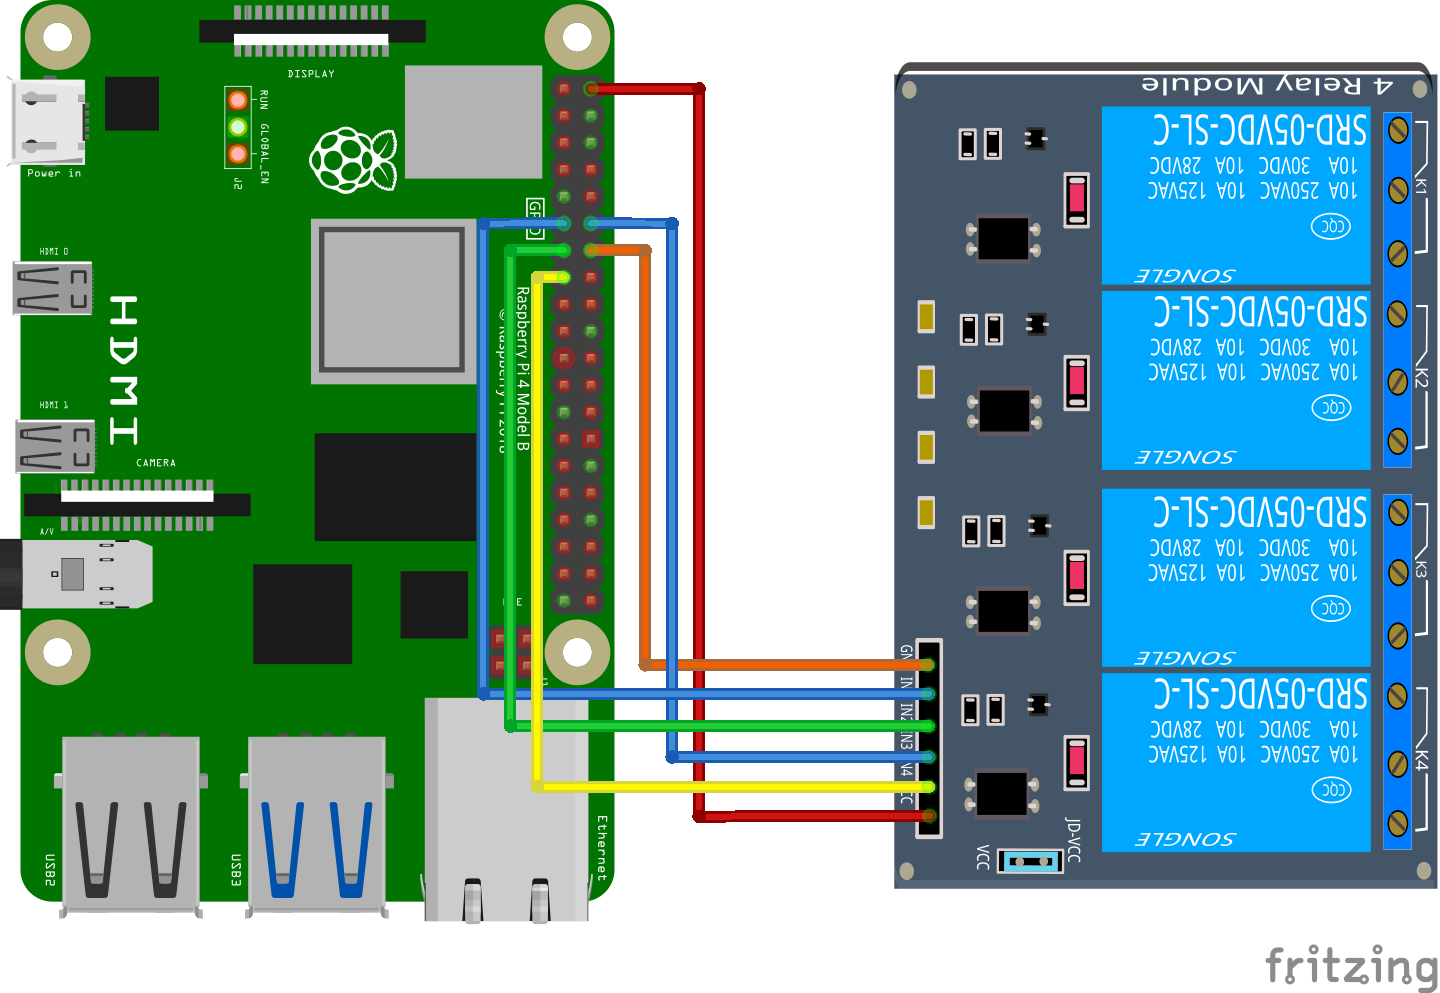
\includegraphics[scale=0.7]{figures/hcis/4ch_relai.png}
			\caption{Anschlussplan Relais}
			\label{fig:output}
	\end{center}
\end{figure}

\subsection{Software}

Wichtig bei der Programmierung war in diesem Fall die dauerhafte Verfügbarkeit der Grundfunktionen  sowie die einfache Integrierbarkeit von alten und neuen Bauteilen. Dies wurde erreicht durch die Anwendung verschiedener Bibliotheken.\\
Die Wichtigsten in dieser Anwendung waren: \\

\subsubsection{gpiozero}

Eine Bibliothek, welche das einfache und schnelle Integrieren neuer Ein- oder Ausgänge ermöglicht. Dadurch können schnell und einfach Änderungen an dem Steuerverhalten der Peripherie gemacht werden. Hierzu kann die Klasse Button und DigitalOutputDevice verwendet werden. Dieser können Parameter wie die gewünschte Debounce Zeit und verwendete Pull-Widerstände übergeben werden. Es werden nur drei Zeilen Code benötigt um einen Aus- oder Eingang zu definieren und anzusteuern \footnote{siehe: Anhang}

\subsubsection{threading}

Eine Bibliothek, welche es ermöglicht, einen eigenen Thread \footnote{gleichzeitig laufende Aufgabe} für das Programm zu öffnen, wodurch die Anwendung ohne Einflüsse oder Unterbrechungen anderer Programme weiter arbeiten kann. Der folgende Programmcode zeigt einen Ausschnitt der Klasse zum Steuern der GPIOs. 

\begin{lstlisting}[language=Python, caption={Code zum Starten eines Threads},captionpos=b]
	
	def start(self):
		self.thread=Thread(target=self.runner)
		self.thread.daemon=True
		self.thread.start()

\end{lstlisting}

In diesem Beispiel wird ein Demon Thread erzeugt und gestartet. Das beutetet dieser Thread wird beim schließen des Programms automatisch mit geschlossen und muss dadurch nicht mehr überwacht werden. Das Target ist die Funktion, welche unabhängig ausgeführt werden soll.

\newpage

%% Benutzeroberfläche %%%%%%%%%%%%%%%%%%%%%%%%%%%%%%%%%%%%%%%

\section{Benutzeroberfläche}
Die Benutzeroberfläche stellt die Verbindung zwischen dem Nutzer und dem Motorrad dar. Sie sollte während der Fahrt die Instrumententafel des Motorrades ersetzen und dem Nutzer die wichtigsten Fahrinformationen anzeigen. Sobald das Motorrad zum Stillstand gekommen ist, wird es möglich Einstellungen zu ändern und die aufgezeichneten Fahrdaten anzeigen zu lassen. Ebenso können der Akkuladestatus und Informationen über Fehler im System entnommen werden.

\subsection{Hardware}

Zur Anzeige und Bedienung wird ein 11.6 Zoll kapazitives Touch LCD Display verwendet. Es besitzt eine Full HD Auflösung (1920x1080), was für eine professionelle Darstellung essentiell ist. Ebenso hat es ein schützendes ABS Gehäuse, welches trotz fehlender IP Zertifizierung das Abdichten ermöglicht. Die Versorgungsspannung beträgt 12V, was ident zu den anderen Komponenten am Motorrad ist und daher die Versorgung sehr vereinfacht, es kann also über den gleichen Spannungswandler versorgt werden.

\begin{figure}[H]
	\begin{center}
		\includegraphics[scale=0.45]{figures/hcis/display_maße.png}
		\caption{Paneel Maße}
		\label{fig:panel}
	\end{center}
\end{figure}

Die Auflösung und die Größe des Paneels wirkt sich stark auf das Design der Benutzeroberfläche aus. Es muss die Größe der Icons und der anderen Designelemente so angepasst werden, dass sie einerseits gut ersichtlich und andererseits einfach über Berührung zu bedienen sind.\\

\newpage

\subsubsection{Befestigung}
Besser: In das Gehäuse des Paneels sind M4 Verschraubungen in einem Raster von 75mm x 75mm integriert und kann daher einfach an Wänden oder Platten verschraubt werden. Um den Bildschirm nun in einer ähnlichen Position wie die Instrumententafel zu befestigen wurde eine 100mm x 210mm x 1.5mm Aluminium Platte - wie in der Abbildung zu sehen - gebogen und mit Löchern versehen. Um diese Halterung nun an dem Motorrad zu befestigten werden die Verschraubungen der alten Instrumententafel verwendet.

\begin{figure}[H]
	\begin{center}
		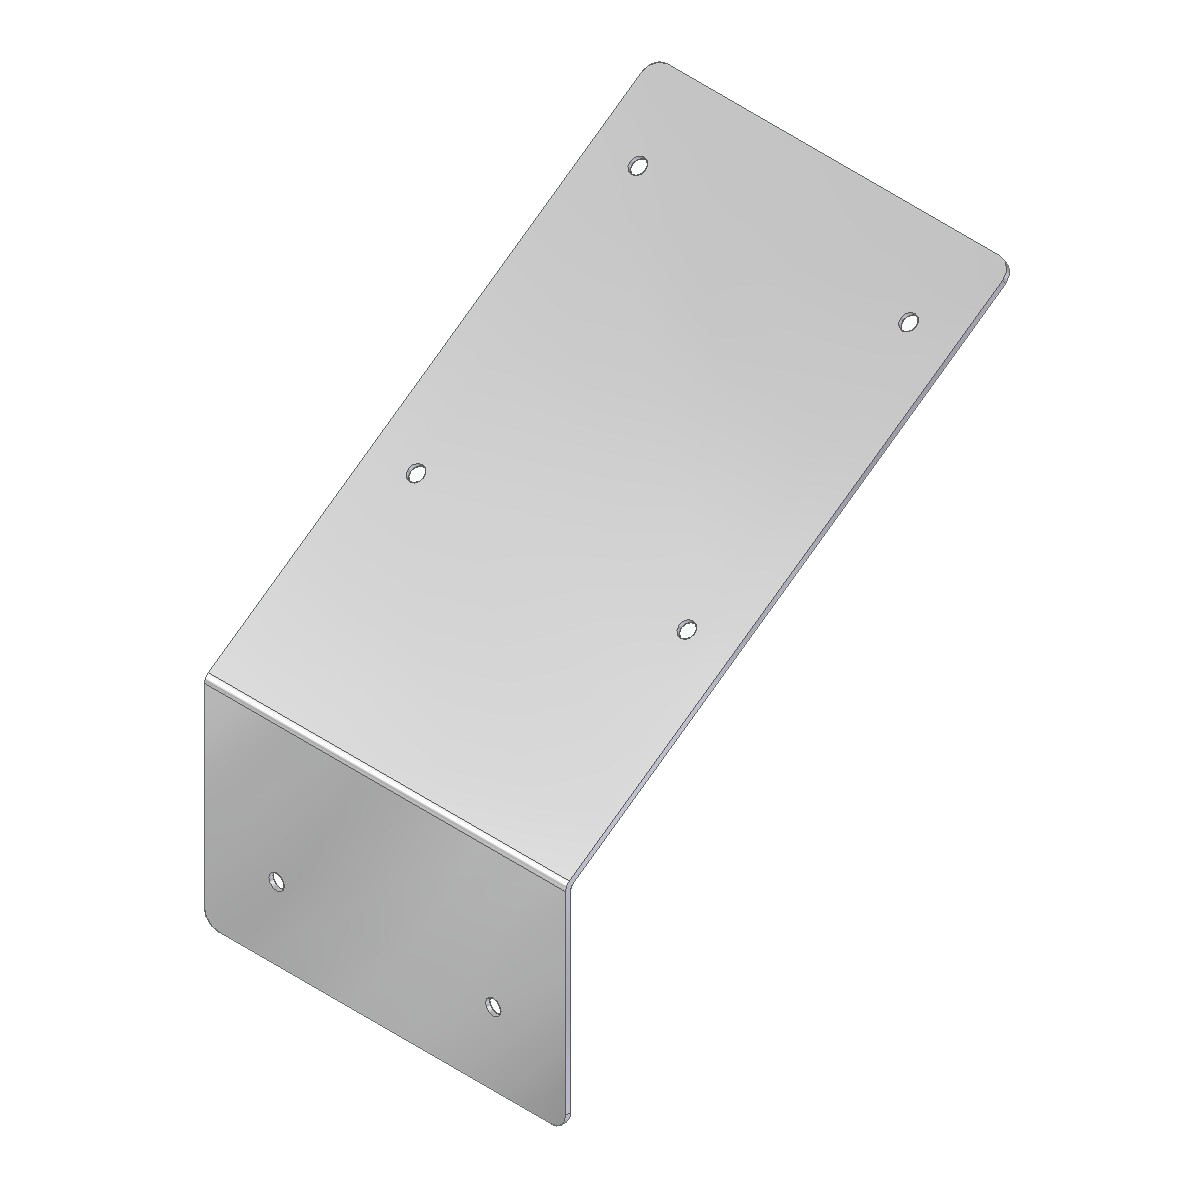
\includegraphics[scale=0.18]{figures/hcis/befestigung_display.png}
		\caption{Befestigung des Displays}
		\label{fig:befestigung}
	\end{center}
\end{figure}

\subsection{Software}
Bevor die Software für die Benutzeroberfläche verfasst wurde, mussten das Design, die Funktionen sowie die angezeigten Informationen geplant werden, um einen reibungslosen Arbeitsablauf beim Entwickeln des Frontends zu gewährleisten. Design Elemente wurden zuvor in Adobe Illustrator vorgefertigt. In den folgenden Seiten wird das Ergebnis dieses Prozesses erläutert.
\subsubsection{Aufbau}
Die nachfolgende Abbildung zeigt den grundsätzlichen Programmaufbau der Benutzeroberfläche. Die einzelnen Fenster werden als Tabelle mit ihren angezeigten Informationen dargestellt. Dies is wichtig da jede dieser Informationen vom Backend an das Frontend gesendet werden müssen.\\
Ebenso sind in den letzten Zeilen der Tabellen die QML-Elemente  zur Navigation zwischen den einzelnen Fenstern niedergeschrieben. Diese müssen auch schon in der frühen Phase der Entwicklung der Benutzeroberfläche definiert werden.

\begin{figure}[H]
	\begin{center}
		\includegraphics[scale=0.4]{figures/hcis/gui_aufbau.png}
		\caption{Aufbau der Graphischen Benutzeroberfläche}
		\label{fig:aufbauGUI}
	\end{center}
\end{figure}

\newpage

\subsubsection{Nutzer / Berechtigungen}

\subsection{Komponenten}

Komponenten sind wiederverwendbare, gekapselte QML-Elemente mit genau definierten Schnittstellen. Komponenten werden häufig durch Komponenten-Dateien definiert, das heißt durch QML-Dateien. Wichtig ist dabei die Definition von Schnittstellen sowie Properties und Signals .

\textbf{Properties}\\
\vspace{2mm}

Einer Property eines Objektes kann ein statischer Wert zugewiesen werden, der konstant bleibt, bis ihm explizit ein neuer Wert zugewiesen wird. Um QML und seine integrierte Unterstützung für dynamisches Objektverhalten optimal zu nutzen, verwenden die meisten QML-Objekte jedoch Propertysbindings.\\
Dies sind eine Kernfunktion von QML, mit der Beziehungen zwischen verschiedenen Objekteigenschaften festgelegt werden können. Wenn sich die Abhängigkeiten einer Property im Wert ändern, wird die Eigenschaft automatisch gemäß der angegebenen Beziehung aktualisiert.\\
Hinter den Kulissen überwacht die QML-Engine die Abhängigkeiten der Eigenschaft. Wenn eine Änderung erkannt wird, wertet die QML-Engine den Bindungsausdruck erneut aus und wendet das neue Ergebnis auf die Eigenschaft an.

\textbf{Java-Script-Funktionen}\\
\vspace{2mm}

Programmlogik kann auch in Java-Script-Funktionen definiert werden. Diese können in QML-Dokumenten definiert und von Signalhandlern, Eigenschaftsbindungen oder Funktionen in anderen QML-Objekten aufgerufen werden. Solche Methoden werden häufig als Inline-Java-Script-Funktionen bezeichnet, da ihre Implementierung im QML-Dokument statt in einer externen Java-Script-Datei enthalten ist.

\subsubsection{Navigationsmenü}

Das Navigations-Menü ist ein Dropdown-Menü, welches zur Navigation zwischen den verschiedenen Fenstern benützt wird. Sobald man sich eingeloggt hat wird das Menü angezeigt und die einzelnen Untermenüs können aufgerufen werden. Das Menü wird abhängig von den Berechtigungen des Benutzers angepasst.

\begin{figure}[H]
	\begin{center}
		\includegraphics[scale=0.2]{figures/hcis/component_menu.png}
		\caption{GUI Komponente - Navigation Menü}
		\label{fig:kompNavigation}
	\end{center}
\end{figure}

\textbf{Buttons} \\
\vspace{2mm}
Die Navigation wird über das QML-Element \textit{Mousearea}, welche direkt über den Icons der einzelnen Navigationselemente platziert wurde, gesteuert. Nun kann mit dem Befehl \textit{onClicked} eine Funktion aufgerufen werden, welche das gewünschte Fenster sichtbar macht, sowie das Navigationsmenü wieder nach oben fahren lässt.\\
In dieser Funktion wird ebenso die Berechtigung des Nutzers über eine Globale Variable, welche beim Anmelden durch ein Signal gesetzt wird, abgefragt. Falls die Berechtigung die ausgewählte Funktion nicht zulässt wird ein Informationstext ausgegeben und das Menü wiederum geschlossen.\

\textbf{Abmelden} \\
\vspace{2mm}

Wird der Abmeldebutton gedrückt, werden die Anmeldeinformationen zurückgesetzt und dem Nutzer wird wieder das Anmeldefenster angezeigt, wo er sich nun mit anderen Anmelde-Informationen einloggen kann.

\newpage

\subsubsection{Balken Anzeige}

Die Komponente Balken Anzeige wird in der Benutzeroberfläche zur Visualisierung verschiedener Daten verwendet. Mit ihr können diese übersichtlicher Dargestellt werden. Diese Komponente wird in mehreren QML-Dateien verwendet, daher sind Properties zur Anpassung notwendig. Die wichtigsten davon sind:

\begin{itemize}
	\item Wert - Der Aktuelle Wert, welcher am Balken angezeigt werden sollte.
	\item Anfangswinkel - Der Winkel an dem der Balken entspringt.
	\item maximaler Wert - Der maximal zu erreichende Wert. Dieser Bestimmt die Länge des Hintergrundbalkens
	\item Hintergrundfarbe - Farbe des Hintergrundbalkens (in der Abbildung grau)
	\item Balkenfarbe -Farbe des Anzeigebalkens (in der Abbildung blau)
\end{itemize}

\begin{figure}[H]
	\begin{center}
		\includegraphics[scale=0.5]{figures/hcis/component_bar.png}
		\caption{GUI Komponente - Balken Anzeige}
		\label{fig:kompBalken}
	\end{center}
\end{figure}

Über ein \textit{Signal} kann nun über das Backend der Wert des Balkens verändert werden und in Echtzeit angezeigt werden.

\subsubsection{Modus Anzeige}
Diese Komponente befindet sich auf der Instrumenten Tafel. Der Modus kann über einen Button am Lenker, welcher mit der Curtis Steuerung verbunden ist, geändert werden. Sie dient zum Anzeigen der derzeitig gewählten Fahrmodi und wird über ein \textit{Signal} aus dem Backend gesteuert, welches mit der Listener Klasse verbunden ist.

\begin{figure}[H]
	\begin{center}
		\includegraphics[scale=0.4]{figures/hcis/component_mode.png}
		\caption{GUI Komponente - Modus Anzeige}
				\label{fig:kompModus}
	\end{center}
\end{figure}

Die Modus Anzeige ist eine einfache Komponente. Sie ist ein Item QML-Typ, dadurch wird das Nutzen von \textit{States} möglich. Durch diese können verschiedene Eigenschaften gespeichert und über einen kurzen Befehl wiederhergestellt werden.\\
In diesem Fall wird der Punkt ausgefüllt und die Farbe des Textes geändert.

\newpage

\subsubsection{Graph} \label{sec:graph}

Die Graph Komponente befindet sich auf dem Diagnose Fenster und dient zum Anzeigen der in der Datenbank gespeicherten Fahrdaten. Sie verfügt über einen Ladebalken, welcher nach dem Auswählen der anzuzeigenden Daten den Fortschritt des Auslesens der Datenbank anzeigt. Dieses Auslesen läuft über eine Funktion der Fetcher Klasse.

\begin{figure}[H]
	\begin{center}
		\includegraphics[scale=0.3]{figures/hcis/component_graph.png}
		\caption{GUI Komponente - Graph}
				\label{fig:kompGraph}
	\end{center}
\end{figure}

Realisiert wurde diese Komponente über öffentliche Bibliothek \textit{Charts.js} (Referenz), welche durch die Java Script Unterstützung von \textit{QT}, mit der Installation eines Adapters mit dem QML Programm kompatibel ist. Dadurch wird nun das Zeichnen von verschiedensten Graphen ermöglicht.

\subsubsection{Weitere Komponenten}

Wie schon bei der Fahr Modi Komponente, wurden weitere Objekte, welche zwischen zwei Zuständen hin und her gestalten werden müssen oder eine bestimmte Handlung ausführen sollten, über eine eigene QML Komponente verwirklicht. Diese Ermöglicht nun wiederum das wiederholte verwenden dieser Komponente, sowie das Ansteuern über \textit{States} und \textit{Signale}.\\
Diese Komponenten sind:

\textbf{Umschaltkomponenten}\\
Dies sind Komponenten, welche über ein \textit{Signal} angesteuert werden und dann mithilfe von \textit{States} ihr Aussehen verändern.

\begin{itemize}
	
	\item Blinker Rechts
	\item Blinker Links
	\item Tagfahrlicht
	\item Fernlicht
	
\end{itemize}

\textbf{Touch Komponenten}\\
Dies sind Komponenten, welche eine \textit{Mousearea} mit einer Graphik verbindet. Wird diese Komponente nun mit einem Mausklick ausgewählt, kann eine Funktion ausgeführt oder ein \textit{Signal} ausgesendet werden.

\begin{itemize}
	
	\item Abmeldebutton
	\item Navigationsmenübuttons
	\item Menü-Öffnen-Button
	
\end{itemize}

\newpage

\subsection{Programm Fenster}

\subsubsection{Login}

Das Login Fenster dient zur Autorisierung des Benutzers. Über die User \textit{Kombobox} kann der gewünschte Nutzer mit der dazugehörigen Berechtigung ausgewählt werden (siehe Abschnitt ). Das Fenster dient ebenso zur Darstellung der Logos unserer Sponsoren\\

\begin{figure}[H]
	\begin{center}
		\includegraphics[scale=0.25]{figures/hcis/window_login.png}
			\caption{GUI Fenster - Login Menü}
			\label{fig:pageMenu}
	\end{center}
\end{figure}

 Um sich einzuloggen muss nur mehr das Passwort im \textit{Textfeld} darunter eingegeben werden. Nach dem Drücken des Login Pfeiles (Neben dem Passwort Textfeld) werden die Login Daten an das Backend versendet. Diese vergleicht die Daten über die Datenbankschnittstelle\footnote{siehe Abschnitt} und loggt, insofern das richtige Passwort gegeben ist, den Benutzer ein. Wird jedoch das Passwort falsch eingegeben, wird eine rote Fehlermeldung angezeigt.\\
 
\subsubsection{Fahrdaten}		

Dieses Fenster dient als Ersatz für die Instrumententafel des Motorrades. Es ist daher das einzige während der Fahrt ersichtliche Fenster. Es Zeigt alle wichtigen Fahrdaten wie Leistung, Geschwindigkeit und Akkuladestand, sowie den Aktuellen Fahrmodus an. Diese Anzeige kann jedem Nutzer, unabhängig der Berechtigung, angezeigt werden.

\begin{figure}[H]
	\begin{center}
		\includegraphics[scale=0.25]{figures/hcis/window_dashboard.png}
			\caption{GUI Fenster - Fahrdaten}
			\label{fig:pageDash}
	\end{center}
\end{figure}

Der Status der Blinker und der Beleuchtung wird ebenso wie die Temperaturen der verschiedenen Komponenten des Motorrades angezeigt. Derzeit ist diese Ansicht starr und kann noch nicht geändert werden. Doch es ist geplant in Zukunft weitere Designs, welche in den Einstellungen geändert werden können, zu implementieren.

\newpage

\subsubsection{Akku- und Ladedaten}

Dieses Fenster dient Ähnlich wie das der Fahrdaten zur Darstellung wichtiger Daten. Es können alle wichtigen Daten bezüglich Akku und BMS auf einem Blick abgelesen werden. 

\begin{figure}[H]
	\begin{center}
		\includegraphics[scale=0.25]{figures/hcis/window_battery.png}
			\caption{GUI Fenster - Akkudaten}
			\label{fig:pageAkku}
	\end{center}
\end{figure}

Dieses Fenster wird Standardmäßig während dem Laden des Fahrzeuges angezeigt. Es benötigt also keine bestimmte Berechtigung und kann von jedem Nutzer über das Navigations-Menü angezeigt werden.

\subsubsection{Fahrdaten Diagnose}

Hier können die Fahrdaten, welche während der Fahrt dauerhaft von der Motorsteuerung versendet und vom Raspberry Pi verarbeitet und in einer Datenbank gespeichert werden, in Graphen angezeigt werden. Hierzu wird die \textit{Graph Komponente} \footnote{siehe Abschnitt \ref{sec:graph}} verwendet.
\begin{figure}[H]
	\begin{center}
		\includegraphics[scale=0.25]{figures/hcis/window_diagnosis.png}
			\caption{GUI Fenster - Fahrdaten Diagnose}
			\label{fig:pageDiagnose}
	\end{center}
\end{figure}

 Diese wird, um während der Fahrt die volle Prozessorleistung zu gewährleisten, erst auf Knopfdruck geladen. In der Menüleiste am unteren Ende des Fensters können verschiedene Vorlagen ausgewählt werden, welche über fixe Datensätze verfügen. Das bedeutet es werden erst beim Auswählen des anzuzeigenden Datensatzes die Daten der letzten Stunde ausgelesen und in den Graphen geladen.


\newpage

\subsubsection{Fehler}

\begin{figure}[H]
	\begin{center}
		\includegraphics[scale=0.25]{figures/hcis/window_error.png}
			\caption{GUI Fenster - Fehler Liste}
			\label{fig:pageError}
	\end{center}
\end{figure}

\subsubsection{Nutzer und Berechtigungen}

Um sicherzustellen das das Nutzen der Benutzeroberfläche nicht für jeden uneingeschränkt möglich ist wurde ein Anmeldesystem mit drei verschiedenen Benutzern, welche jeweils verschiedene Berechtigungen besitzen, umgesetzt.

{\small \textbf{ADMIN}} - Passwort: 53AC2\\

Dieser Benutzer verfügt über uneingeschränkte rechte und kann auf jede Verfügbare Funktion sowie Funktionen, welche noch in Entwicklung sind zugreifen.

{\small \textbf{USER}} - Passwort: 5AHET\\

{\small \textbf{GUEST}} - Passwort: 00000\\


\newpage

\subsection{Realisierung der Benutzeroberfächer}

\subsubsection{QML} \label{sec:qml}
QML \footnote{Qt Modeling Language} ist eine deklarative Sprache, mit der Benutzeroberflächen anhand ihrer visuellen Komponenten und ihrer Interaktion und Beziehung zueinander beschrieben werden können. Es ist eine gut lesbare Sprache, die entwickelt wurde, um die dynamische Verbindung von Komponenten zu ermöglichen und die die einfache Wiederverwendung und Anpassung von Komponenten innerhalb einer Benutzeroberfläche erlaubt. Es bietet  Syntax mit Unterstützung für Java-Script-Ausdrücke in Kombination mit dynamischen Eigenschaftsverbindungen.

\subsubsection{Qt-Quick}
Das Qt-Quick-Modul ist die Standardbibliothek zum schreiben von QML-Anwendungen. Während das QML-Modul die Engine und die Sprachinfrastruktur bereitstellt, bietet das Qt Quick-Modul alle grundlegenden Typen, die zum Erstellen von Benutzeroberflächen mit QML erforderlich sind. Es bietet eine visuelle Zeichenfläche und Typen zum Erstellen und Animieren visueller Komponenten, zum Empfangen von Benutzereingaben, zum Erstellen von Datenmodellen und Ansichten sowie zum verzögerten Objektinstanziieren. Es können problemlos flüssige, animierte Benutzeroberflächen in QML erstellt werden. Diese Benutzeroberflächen können mit beliebigen Backend Bibliotheken verbunden werden.

\subsubsection{Slots und Signals} \label{sec:slots}
Slots und Signals werden in QML zur ereignisgesteuerten Kommunikation zwischen Frontend und Backend verwendet. In der folgenden Illustration wird diese anhand eines einfachen Beispiels erklärt.

\begin{figure}[H]
	\begin{center}
		\includegraphics[scale=0.4]{figures/hcis/signals_slots.png}
		\caption{Slots und Signals Konzept}
	\end{center}
\end{figure}

\textbf{Signale}\\ \medskip
Diese können als Mitteilungen angesehen werden, welche über das Aufrufen der \textit{signal.emit()} Funktion vom Backend an das Frontend gesendet wird. Im Frontend wird wiederum eine eigens definierte Funktion benötigt um dem Wert einem Property eines QML Elements zuzuweisen.
\medskip

\textbf{Slots}\\ \medskip
Slots sind Call-Back Funktionen, welche im Backend definiert werden und sind über die Bridge Klasse mit dem Frontend verknüpft. Dadurch können diese Funktionen im Frontend aufgerufen und mit Signalen verbunden werden. Sie stellen daher die wichtigste Verbindung zwischen dem Programm und der Benutzeroberfläche dar.

\newpage
	
\subsubsection{Bridge}

Die Bridge Klasse wird für die Kommunikation zwischen den einzelnen Module des Backends mit denen der graphischen Benutzeroberfläche. 

\begin{figure}[H]
	\begin{center}
		\includegraphics[scale=1]{figures/hcis/bridge.png}
		\caption{Verbindung Frontend zu Backend}
	\end{center}
\end{figure}

\newpage

%% Kommunikation %%%%%%%%%%%%%%%%%%%%%%%%%%%%%%%%%%%%%%%%%%%%

\section{Kommunikation}

Um Daten zwischen den mehreren Steuereinheiten des Motorrades zu versenden, muss eine Echtzeit-Kommunikation über ein Bussystem gewährleistet werden. Die Entscheidung ist auf das Controller Area Network Bussystem (CAN-Bus) gefallen. Ausschlaggebend für diese Entscheidung war der Curtis Motorcontroller, dieser verfügt über eine serielle Schnittstelle (RS-232) sowie ein CAN-System. Für unserer Anwendung bietet das CAN-System eine größere Ausbaufähigkeit sowie größere Übertragungsraten, weshalb wir uns letztendlich auch dafür entschieden haben.

\subsection{Hardware}

\subsubsection{CAN-Modul}

Da der Raspberry Pi selbst nicht über ein CAN-System verfügt, erfolgt der Anschluss an die Busleitung über ein externes CAN-Modul, welches über das Serial Peripheral Interface (SPI) mit dem Raspberry Pi kommuniziert, welches wie folgt angeschlossen werden muss: 

\begin{figure}[H]
	\begin{center}
		\includegraphics[scale=0.9]{figures/hcis/can_module.png}
		\caption{Anschlussplan CAN-Modul}
	\end{center}
\end{figure}

Die Kommunikation wird über zwei Komponenten ermöglicht. Einen MCP2562 Transceiver, welcher für die Verarbeitung der Nachrichten zuständig ist und ein MCP2515 CAN Interface, welches die Daten zwischenspeichert und sich um das Versenden der Nachrichten kümmert. Gemeinsam mit dem Mikrocomputer ergibt dies nun einen CAN Node, welcher fähig ist Nachrichten zu versenden und zu empfangen.

\subsubsection{Netzwerkstruktur}

Ein CAN-Netzwerk wird standardmäßig als Bus- oder Sterntopologie aufgebaut. Wir haben uns bewusst für die Bustopologie entschieden, da Sterntopologien nur in bestimmten Anwendungen Gebrauch finden und noch dazu markante Nachteile besitzt.\\ Es müsste zum Beispiel eine zentrale Steuereinheit den Nachrichtenverkehr steuern, ebenso gibt uns die niedrige Anzahl an Teilnehmern im Netzwerk nicht einmal die Möglichkeit ein anderes System zu verwenden. Erst wenn wir in Zukunft das CAN-Netzwerk um Sensoren und Aktoren erweitern würden, müsste weitere Zeit in die Planung des Netzwerks investiert werden. 

\newpage

\subsection{Listener}

Die Listener Klasse ist dafür zuständig den Datenverkehr am Bus zu überwachen und geordnet an die Datenbankschnittstelle (Fetcher) sowie die Schnittstelle zum Frontend (Bridge) weiterzugeben.

\subsubsection{Konfigurieren der Schnittstelle}
	
\begin{lstlisting}[language=Python, caption={Konfigurieren des CAN Adapters},captionpos=b]
	
	def start(self):
	self.thread=Thread(target=self.runner)
	self.thread.daemon=True
	self.thread.start()
	
\end{lstlisting}

\subsubsection{Empfangen der Daten}

\newpage

%% Fahrdatenspeicher %%%%%%%%%%%%%%%%%%%%%%%%%%%%%%%%%%%%%%%%

\section{Fahrdatenspeicher}

Das Motorrad sollte seine Fahrdaten abspeichern und darstellen können, um eine Diagnose des gesamten Aufbaus zu gewährleisten. Dafür wird eine Datenbank verwendet, nämlich die weit verbreitete Software mySQL verwendet.

\subsection{Datenbankstruktur}

\subsubsection{Benutzer System}

\begin{table}[H]
	\begin{center}
		\begin{tabular}{|c|c|l|}
		\hline
		\multicolumn{3}{|c|}{\textbf{users}}                          \\ \hline
		\textbf{Attribut} & \textbf{Datentyp} & \textbf{Beschreibung} \\ \hline
		id                & int               & Identifikationsnummer \\ \hline
		username          & varchar(50)       & Name des Benutzers    \\ \hline
		password          & varchar(255)      & Eingegebenes Passwort \\ \hline
		\end{tabular}
		\caption{Datenbankstruktur der Benutzer Tabelle}
		\label{tab:logindata}
	\end{center}
\end{table}

\subsubsection{Motor Daten}

\textbf{Datenpacket 1}
 
\begin{table}[H]
	\begin{center}
		\begin{tabular}{|c|c|l|}
			\hline
			\multicolumn{3}{|c|}{\textbf{data1}} \\ \hline
			\textbf{Attribut} & \textbf{Datentyp} & \textbf{Beschreibung}            \\ \hline
			id                & int               & Identifikationsnummer            \\ \hline
			date\_time        & datetime          & Datum der Erstellung             \\ \hline
			vehicle\_speed    & int               & Geschwindigkeit des Motorrades   \\ \hline
			current\_rms      & int               & Ausgangsstrom der Motorsteuerung \\ \hline
			controller\_temp  & int               & Temperatur des Kontrollers       \\ \hline
			motor\_temp       & int               & Temperatur des Motors            \\ \hline
			motor\_torque     & int               & Drehmoment am Motor              \\ \hline
			modulation\_depth & int               & Modulationsgrad des Kontrollers  \\ \hline
		\end{tabular}
			\caption{Datenbankstruktur der Datenpaket 1 Tabelle}
			\label{tab:data1}
	\end{center}
\end{table}

\newpage

\textbf{Datenpacket 2}

\begin{table}[H]
	\begin{center}
		\begin{tabular}{|c|c|l|}
			\hline
			\multicolumn{3}{|c|}{\textbf{data2}} \\ \hline
			\textbf{Attribut}  & \textbf{Datentyp} & \textbf{Beschreibung}               \\ \hline
			id                 & int               & Identifikationsnummer               \\ \hline
			id\_data\_1        & int               & Fremdschlüssel von Datenpacket 1    \\ \hline
			date\_time         & datetime          & Datum der Erstellung                \\ \hline
			vehicle\_speed     & int               & Geschwindigkeit des Motorrades      \\ \hline
			capacitator\_volts & int               & Eingangsspannung der Motorsteuerung \\ \hline
			bdi\_percentage    & int               &                                     \\ \hline
			interlock          & int               &                                     \\ \hline
			throttle\_command  & int               & Stellung des Gasgriffes             \\ \hline
			brake\_command     & int               & Stellung der Motorbremse (software) \\ \hline
			emr\_state         & int               &                                     \\ \hline
		\end{tabular}
			\caption{Datenbankstruktur der Datenpaket 2 Tabelle}
			\label{tab:data2}
	\end{center}
\end{table}

\textbf{Datenpacket 3}

\begin{table}[H]
	\begin{center}
		\begin{tabular}{|c|c|l|}
			\hline
			\multicolumn{3}{|c|}{\textbf{data3}} \\ \hline
			\textbf{Attribut}           & \textbf{Datentyp} & \textbf{Beschreibung}                     \\ \hline
			id                          & int               & Identifikationsnummer                     \\ \hline
			id\_data\_2                 & int               & Fremdschlüssel von Datenpacket 2          \\ \hline
			date\_time                  & datetime          & Datum der Erstellung                      \\ \hline
			vehicle\_speed              & int               & Geschwindigkeit des Motorrades            \\ \hline
			vehicle\_accelration        & int               & Eingangsspannung der Motorsteuerung       \\ \hline
			vehicle\_odometer           & int               & Vom Motorrad zurückgelegte Strecke        \\ \hline
			time\_to\_capture\_speed    & int               & Zeit bis zur eingestellten Geschwindikeit \\ \hline
			time\_to\_capture\_distance & int               & Zeit bis zur eingestellten Distanz        \\ \hline
			braking\_distance\_captured & int               & Zeit von Bremsbegin bis zu Stillstand     \\ \hline
			distance\_since\_stop       & int               & Zurückgelegte Distanz seit dem Stillstand \\ \hline
		\end{tabular}
		\caption{Datenbankstruktur der Datenpaket 3 Tabelle}
		\label{tab:data3}
	\end{center}
\end{table}

\newpage

\textbf{Datenpacket 4 - Fehler}

\begin{table}[H]
	\begin{center}
		\begin{tabular}{|c|c|l|}
			\hline
			\multicolumn{3}{|c|}{\textbf{data4}} \\ \hline
			\textbf{Attribut}           & \textbf{Datentyp} & \textbf{Beschreibung}                     \\ \hline
			id                          & int               & Identifikationsnummer                     \\ \hline
			id\_data\_2                 & int               & Fremdschlüssel von Datenpacket 2          \\ \hline
			date\_time                  & datetime          & Datum der Erstellung                      \\ \hline
			vehicle\_speed              & int               & Geschwindigkeit des Motorrades            \\ \hline
			vehicle\_accelration        & int               & Eingangsspannung der Motorsteuerung       \\ \hline
			vehicle\_odometer           & int               & Vom Motorrad zurückgelegte Strecke        \\ \hline
			time\_to\_capture\_speed    & int               & Zeit bis zur eingestellten Geschwindikeit \\ \hline
			time\_to\_capture\_distance & int               & Zeit bis zur eingestellten Distanz        \\ \hline
			braking\_distance\_captured & int               & Zeit von Bremsbeginn bis zu Stillstand     \\ \hline
			distance\_since\_stop       & int               & Zurückgelegte Distanz seit dem Stillstand \\ \hline
		\end{tabular}
		\caption{Datenbankstruktur der Fehler-Datenpaket Tabelle}
		\label{tab:data4}
	\end{center}
\end{table}

\subsubsection{Akku Daten}

\subsection{Handler}

Die Handler Klasse hat die Aufgabe eine Verbindung zwischen der Datenbank und dem Programm herzustellen. Dazu verwendet sie die mySQL connector Bibliothek. Mit dieser können SQL Skripte direkt in die Python Klasse integriert werden ohne dass externe SQL Skript Dateien geöffnet werden müssen. 

\subsubsection{Konfigurieren der Schnittstelle}

\begin{lstlisting}[language=Python, caption={Konfiguration der Datenbankschnittstelle},captionpos=b]
	
	# Database credentials
	dbhost = "localhost"
	dbuser = "root"
	dbpass = "8Yf!97mmnZbvYJe"
	dbname = "login_data"
	
	# Connection to the database
	con = mysql.connector.connect(host=dbhost, user=dbuser, password=dbpass, database=dbname)
	
	# Creating cursor for database queries
	cursor = con.cursor()
	
\end{lstlisting}


\subsubsection{SELECT Befehl}

\subsubsection{INSERT Befehl}

Dieser Befehl kann in zwei Bereiche unterteilt werden. In der ersten Zeile wird die
Zieltabelle mit den Attributen angegeben. In der zweiten Zeile folgen die Werte, die in der Datenbank erfasst werden sollen. Hierbei ist die Reihenfolge der Attribute zu beachten. Das Attribut id wird standardmäßig von dem Datenbanksystem vergeben, es ist daher möglich das Attribut im Befehl zu vernachlässigen. Ebenso unterstützt MySQL als Wert die Funktion \textit{NOW()}, wodurch intern der aktuelle Zeitstempel abgespeichert wird. Dadurch kümmert sich das Datenbanksystem um die korrekten Werte für das date\_time Attribut.

\begin{lstlisting}[language=SQL, caption={Konfiguration der Datenbankschnittstelle},captionpos=b]
	
	INSERT INTO `users` (`id`, `username`, `password`)
	VALUES (1, 'USER', '5AHET');
	INSERT INTO `users` (`id`, `username`, `password`)
	VALUES (2, 'GUEST', '00000');
	INSERT INTO `users` (`id`, `username`, `password`)
	VALUES (3, 'ADMIN', '53AC2');
	
\end{lstlisting}

\newpage

\chapter{Endergebnis}
\fancyfoot[C]{Kronberger, Lackner, Kern, Schmeisser}


%% ANHÄNGE %%%%%%%%%%%%%%%%%%%%%%%%%%%%%%%%%%%%%%%%%%%%%%%%%%

\appendix
\chapter{Arbeitsnachweis}

\section{Zeitplan}

\section{Kosten}

\chapter{Dokumente}

%% LITERATUR UND ANDERE VERZEICHNISSE %%%%%%%%%%%%%%%%%%%%%%%

%% Literaturverzeichnis

\fancyfoot[C]{Kronberger, Lackner, Kern, Schmeisser}

\addcontentsline{toc}{chapter}{Literaturverzeichnis}
\printbibliography

%% Abbildungsverzeichnis

\addcontentsline{toc}{chapter}{Abbildungsverzeichnis}
\listoffigures

%% Tabellenverzeichnis

\addcontentsline{toc}{chapter}{Tabellenverzeichnis}
\listoftables

%% Codeverzeichnis

\addcontentsline{toc}{chapter}{Codeverzeichnis}
\lstlistoflistings

\end{document}